% Options for packages loaded elsewhere
\PassOptionsToPackage{unicode}{hyperref}
\PassOptionsToPackage{hyphens}{url}
\PassOptionsToPackage{dvipsnames,svgnames,x11names}{xcolor}
%
\documentclass[
  letterpaper,
  DIV=11,
  numbers=noendperiod]{scrreprt}

\usepackage{amsmath,amssymb}
\usepackage{iftex}
\ifPDFTeX
  \usepackage[T1]{fontenc}
  \usepackage[utf8]{inputenc}
  \usepackage{textcomp} % provide euro and other symbols
\else % if luatex or xetex
  \usepackage{unicode-math}
  \defaultfontfeatures{Scale=MatchLowercase}
  \defaultfontfeatures[\rmfamily]{Ligatures=TeX,Scale=1}
\fi
\usepackage{lmodern}
\ifPDFTeX\else  
    % xetex/luatex font selection
\fi
% Use upquote if available, for straight quotes in verbatim environments
\IfFileExists{upquote.sty}{\usepackage{upquote}}{}
\IfFileExists{microtype.sty}{% use microtype if available
  \usepackage[]{microtype}
  \UseMicrotypeSet[protrusion]{basicmath} % disable protrusion for tt fonts
}{}
\makeatletter
\@ifundefined{KOMAClassName}{% if non-KOMA class
  \IfFileExists{parskip.sty}{%
    \usepackage{parskip}
  }{% else
    \setlength{\parindent}{0pt}
    \setlength{\parskip}{6pt plus 2pt minus 1pt}}
}{% if KOMA class
  \KOMAoptions{parskip=half}}
\makeatother
\usepackage{xcolor}
\setlength{\emergencystretch}{3em} % prevent overfull lines
\setcounter{secnumdepth}{5}
% Make \paragraph and \subparagraph free-standing
\makeatletter
\ifx\paragraph\undefined\else
  \let\oldparagraph\paragraph
  \renewcommand{\paragraph}{
    \@ifstar
      \xxxParagraphStar
      \xxxParagraphNoStar
  }
  \newcommand{\xxxParagraphStar}[1]{\oldparagraph*{#1}\mbox{}}
  \newcommand{\xxxParagraphNoStar}[1]{\oldparagraph{#1}\mbox{}}
\fi
\ifx\subparagraph\undefined\else
  \let\oldsubparagraph\subparagraph
  \renewcommand{\subparagraph}{
    \@ifstar
      \xxxSubParagraphStar
      \xxxSubParagraphNoStar
  }
  \newcommand{\xxxSubParagraphStar}[1]{\oldsubparagraph*{#1}\mbox{}}
  \newcommand{\xxxSubParagraphNoStar}[1]{\oldsubparagraph{#1}\mbox{}}
\fi
\makeatother

\usepackage{color}
\usepackage{fancyvrb}
\newcommand{\VerbBar}{|}
\newcommand{\VERB}{\Verb[commandchars=\\\{\}]}
\DefineVerbatimEnvironment{Highlighting}{Verbatim}{commandchars=\\\{\}}
% Add ',fontsize=\small' for more characters per line
\newenvironment{Shaded}{}{}
\newcommand{\AlertTok}[1]{\textcolor[rgb]{0.58,0.85,0.30}{\textbf{\colorbox[rgb]{0.30,0.12,0.14}{#1}}}}
\newcommand{\AnnotationTok}[1]{\textcolor[rgb]{0.60,0.76,0.47}{#1}}
\newcommand{\AttributeTok}[1]{\textcolor[rgb]{0.78,0.47,0.87}{#1}}
\newcommand{\BaseNTok}[1]{\textcolor[rgb]{0.82,0.60,0.40}{#1}}
\newcommand{\BuiltInTok}[1]{\textcolor[rgb]{0.78,0.47,0.87}{#1}}
\newcommand{\CharTok}[1]{\textcolor[rgb]{0.60,0.76,0.47}{#1}}
\newcommand{\CommentTok}[1]{\textcolor[rgb]{0.36,0.39,0.44}{\textit{#1}}}
\newcommand{\CommentVarTok}[1]{\textcolor[rgb]{0.88,0.42,0.46}{\textit{#1}}}
\newcommand{\ConstantTok}[1]{\textcolor[rgb]{0.82,0.60,0.40}{#1}}
\newcommand{\ControlFlowTok}[1]{\textcolor[rgb]{0.78,0.47,0.87}{#1}}
\newcommand{\DataTypeTok}[1]{\textcolor[rgb]{0.78,0.47,0.87}{#1}}
\newcommand{\DecValTok}[1]{\textcolor[rgb]{0.82,0.60,0.40}{#1}}
\newcommand{\DocumentationTok}[1]{\textcolor[rgb]{0.64,0.20,0.25}{#1}}
\newcommand{\ErrorTok}[1]{\textcolor[rgb]{0.96,0.28,0.28}{\underline{#1}}}
\newcommand{\ExtensionTok}[1]{\textcolor[rgb]{0.38,0.69,0.94}{\textbf{#1}}}
\newcommand{\FloatTok}[1]{\textcolor[rgb]{0.82,0.60,0.40}{#1}}
\newcommand{\FunctionTok}[1]{\textcolor[rgb]{0.38,0.69,0.94}{#1}}
\newcommand{\ImportTok}[1]{\textcolor[rgb]{0.60,0.76,0.47}{#1}}
\newcommand{\InformationTok}[1]{\textcolor[rgb]{0.77,0.36,0.00}{#1}}
\newcommand{\KeywordTok}[1]{\textcolor[rgb]{0.78,0.47,0.87}{#1}}
\newcommand{\NormalTok}[1]{\textcolor[rgb]{0.67,0.70,0.75}{#1}}
\newcommand{\OperatorTok}[1]{\textcolor[rgb]{0.78,0.47,0.87}{#1}}
\newcommand{\OtherTok}[1]{\textcolor[rgb]{0.15,0.68,0.38}{#1}}
\newcommand{\PreprocessorTok}[1]{\textcolor[rgb]{0.78,0.47,0.87}{#1}}
\newcommand{\RegionMarkerTok}[1]{\textcolor[rgb]{0.16,0.50,0.73}{\colorbox[rgb]{0.08,0.19,0.26}{#1}}}
\newcommand{\SpecialCharTok}[1]{\textcolor[rgb]{0.34,0.71,0.76}{#1}}
\newcommand{\SpecialStringTok}[1]{\textcolor[rgb]{0.85,0.27,0.33}{#1}}
\newcommand{\StringTok}[1]{\textcolor[rgb]{0.60,0.76,0.47}{#1}}
\newcommand{\VariableTok}[1]{\textcolor[rgb]{0.88,0.42,0.46}{#1}}
\newcommand{\VerbatimStringTok}[1]{\textcolor[rgb]{0.85,0.27,0.33}{#1}}
\newcommand{\WarningTok}[1]{\textcolor[rgb]{0.85,0.27,0.33}{#1}}

\providecommand{\tightlist}{%
  \setlength{\itemsep}{0pt}\setlength{\parskip}{0pt}}\usepackage{longtable,booktabs,array}
\usepackage{calc} % for calculating minipage widths
% Correct order of tables after \paragraph or \subparagraph
\usepackage{etoolbox}
\makeatletter
\patchcmd\longtable{\par}{\if@noskipsec\mbox{}\fi\par}{}{}
\makeatother
% Allow footnotes in longtable head/foot
\IfFileExists{footnotehyper.sty}{\usepackage{footnotehyper}}{\usepackage{footnote}}
\makesavenoteenv{longtable}
\usepackage{graphicx}
\makeatletter
\def\maxwidth{\ifdim\Gin@nat@width>\linewidth\linewidth\else\Gin@nat@width\fi}
\def\maxheight{\ifdim\Gin@nat@height>\textheight\textheight\else\Gin@nat@height\fi}
\makeatother
% Scale images if necessary, so that they will not overflow the page
% margins by default, and it is still possible to overwrite the defaults
% using explicit options in \includegraphics[width, height, ...]{}
\setkeys{Gin}{width=\maxwidth,height=\maxheight,keepaspectratio}
% Set default figure placement to htbp
\makeatletter
\def\fps@figure{htbp}
\makeatother

\usepackage{booktabs}
\usepackage{longtable}
\usepackage{array}
\usepackage{multirow}
\usepackage{wrapfig}
\usepackage{float}
\usepackage{colortbl}
\usepackage{pdflscape}
\usepackage{tabu}
\usepackage{threeparttable}
\usepackage{threeparttablex}
\usepackage[normalem]{ulem}
\usepackage{makecell}
\usepackage{xcolor}
\usepackage{svg}
\KOMAoption{captions}{tableheading}
\makeatletter
\@ifpackageloaded{bookmark}{}{\usepackage{bookmark}}
\makeatother
\makeatletter
\@ifpackageloaded{caption}{}{\usepackage{caption}}
\AtBeginDocument{%
\ifdefined\contentsname
  \renewcommand*\contentsname{Table of contents}
\else
  \newcommand\contentsname{Table of contents}
\fi
\ifdefined\listfigurename
  \renewcommand*\listfigurename{List of Figures}
\else
  \newcommand\listfigurename{List of Figures}
\fi
\ifdefined\listtablename
  \renewcommand*\listtablename{List of Tables}
\else
  \newcommand\listtablename{List of Tables}
\fi
\ifdefined\figurename
  \renewcommand*\figurename{Figure}
\else
  \newcommand\figurename{Figure}
\fi
\ifdefined\tablename
  \renewcommand*\tablename{Table}
\else
  \newcommand\tablename{Table}
\fi
}
\@ifpackageloaded{float}{}{\usepackage{float}}
\floatstyle{ruled}
\@ifundefined{c@chapter}{\newfloat{codelisting}{h}{lop}}{\newfloat{codelisting}{h}{lop}[chapter]}
\floatname{codelisting}{Listing}
\newcommand*\listoflistings{\listof{codelisting}{List of Listings}}
\makeatother
\makeatletter
\makeatother
\makeatletter
\@ifpackageloaded{caption}{}{\usepackage{caption}}
\@ifpackageloaded{subcaption}{}{\usepackage{subcaption}}
\makeatother

\ifLuaTeX
  \usepackage{selnolig}  % disable illegal ligatures
\fi
\usepackage{bookmark}

\IfFileExists{xurl.sty}{\usepackage{xurl}}{} % add URL line breaks if available
\urlstyle{same} % disable monospaced font for URLs
\hypersetup{
  pdftitle={A Guide to Interpreting the Results of MetaDAG Analysis},
  colorlinks=true,
  linkcolor={blue},
  filecolor={Maroon},
  citecolor={Blue},
  urlcolor={Blue},
  pdfcreator={LaTeX via pandoc}}


\title{A Guide to Interpreting the Results of MetaDAG Analysis}
\author{}
\date{}

\begin{document}
\maketitle

\renewcommand*\contentsname{Table of contents}
{
\hypersetup{linkcolor=blue}
\setcounter{tocdepth}{2}
\tableofcontents
}

\bookmarksetup{startatroot}

\chapter{Introduction}\label{introduction}

As an illustrative example for interpreting
\href{https://bioinfo.uib.es/metadag/}{metaDAG} results, we consider
here the Eukaryotes test presented in Section 2.5. Namely, we consider
all Eukaryotes from the KEGG database.
\href{https://www.github.com/biocom-uib/metadag}{Experiment github.}

First of all, results must be downloaded from:

Hash:
\href{https://bioinfo.uib.es/metadag/handleExperiment/0a845f74-826e-3b46-aed9-e7ecf74db262}{0a845f74-826e-3b46-aed9-e7ecf74db262}

URL:
(https://bioinfo.uib.es/metadag/handleExperiment/result\_0a845f74-826e-3b46-aed9-e7ecf74db262)

and saved in the folder:

``data/0a845f74-826e-3b46-aed9-e7ecf74db262''.

\begin{Shaded}
\begin{Highlighting}[]
\FunctionTok{library}\NormalTok{(tidyverse)}
\FunctionTok{library}\NormalTok{(igraph)}
\FunctionTok{library}\NormalTok{(ComplexHeatmap)}
\FunctionTok{library}\NormalTok{(viridis)}
\FunctionTok{library}\NormalTok{(circlize)}
\FunctionTok{library}\NormalTok{(plotly)}
\FunctionTok{library}\NormalTok{(randomcoloR)}
\FunctionTok{library}\NormalTok{(factoextra)}
\FunctionTok{library}\NormalTok{(RColorBrewer)}
\FunctionTok{library}\NormalTok{(kableExtra)}
\FunctionTok{library}\NormalTok{(igraph)}
\FunctionTok{library}\NormalTok{(GGally)}
\end{Highlighting}
\end{Shaded}

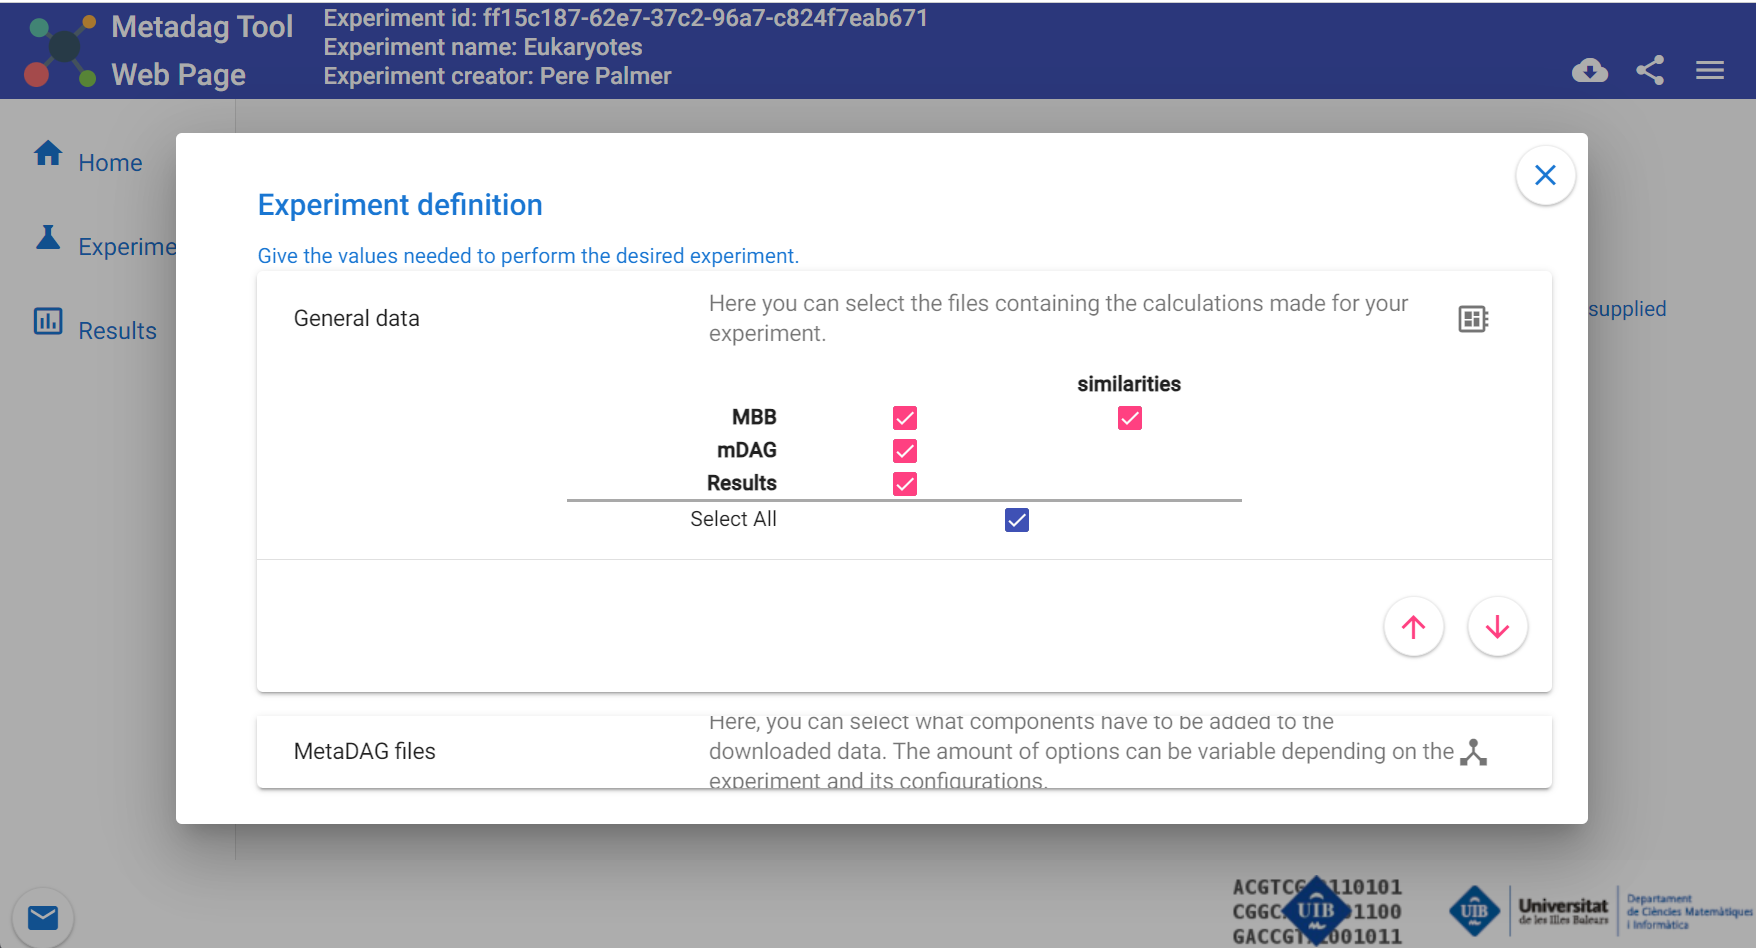
\includegraphics[width=1\textwidth,height=\textheight]{figures/screen_2.png}

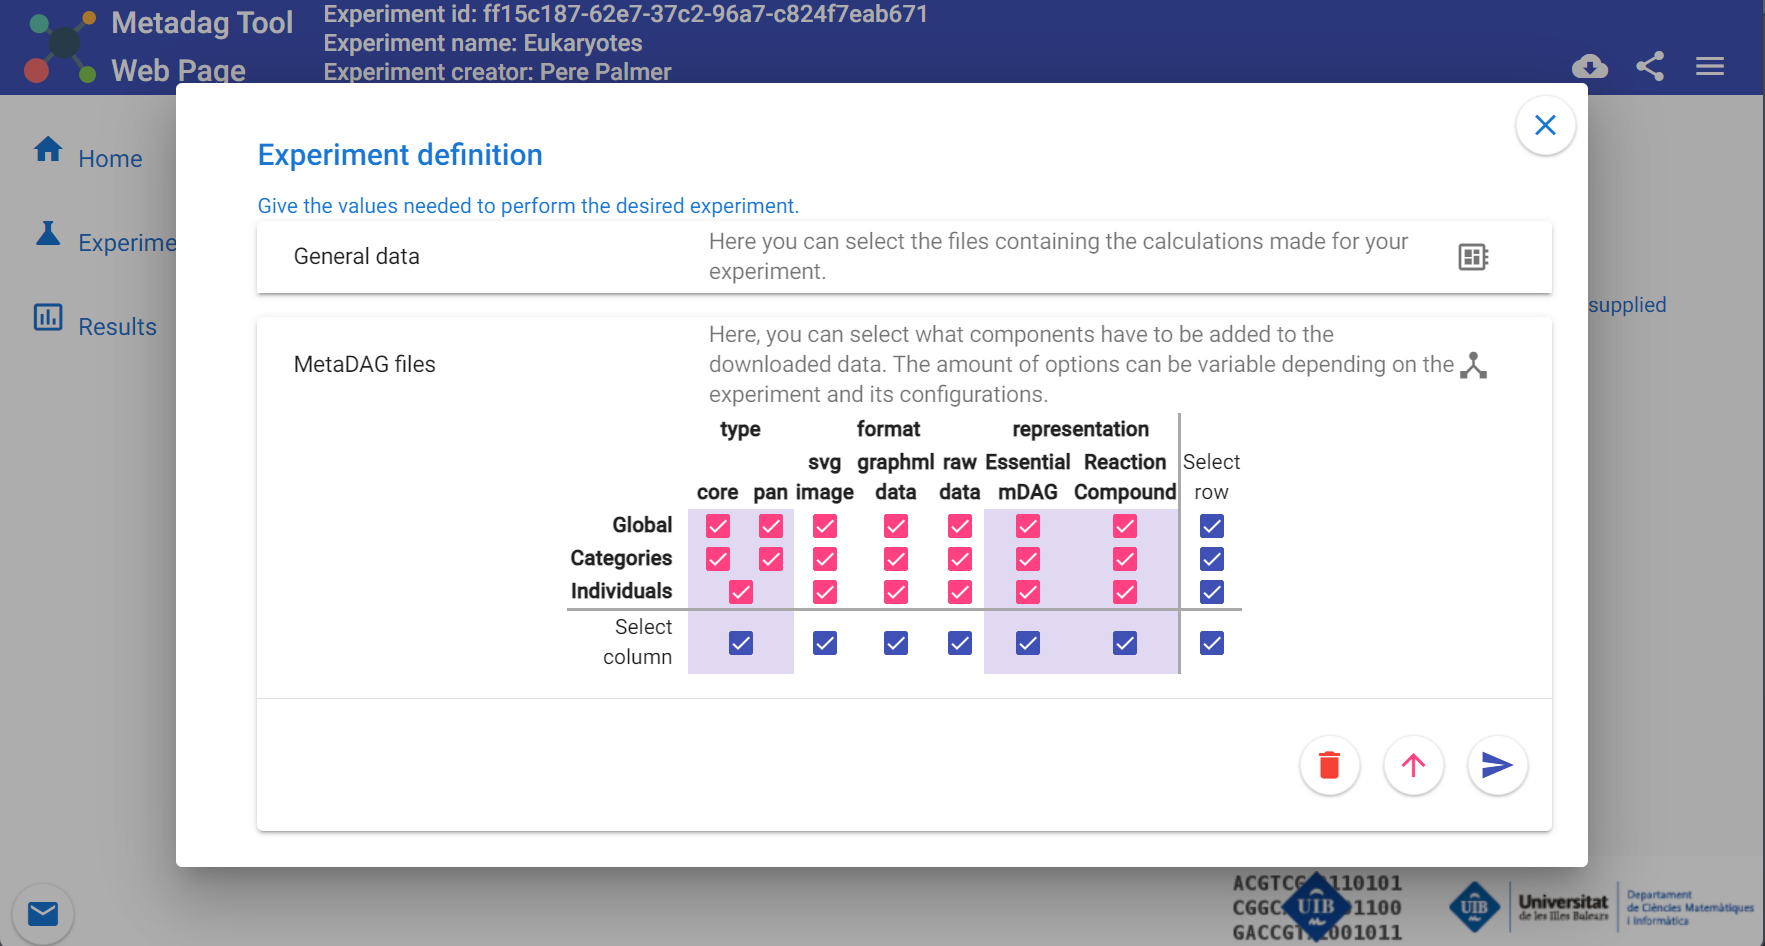
\includegraphics[width=1\textwidth,height=\textheight]{figures/screen_3.png}

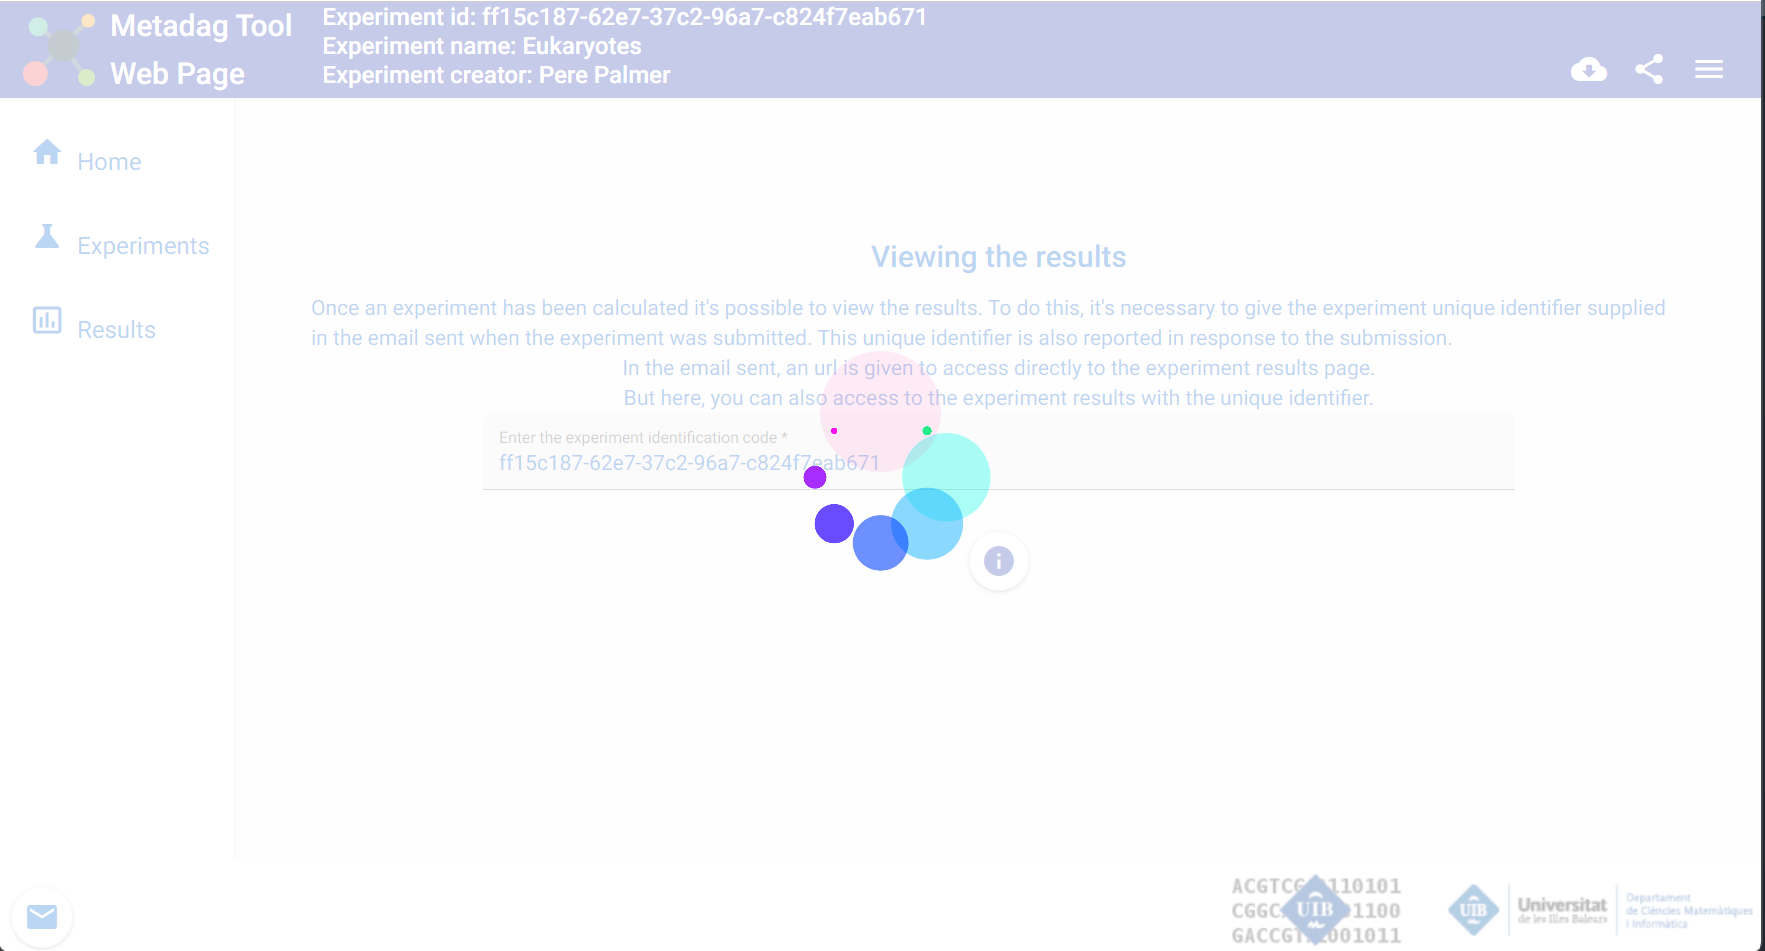
\includegraphics[width=1\textwidth,height=\textheight]{figures/screen_4.png}

\bookmarksetup{startatroot}

\chapter{Load data}\label{load-data}

\begin{Shaded}
\begin{Highlighting}[]
\NormalTok{experiment}\OtherTok{=}
  \StringTok{"0a845f74{-}826e{-}3b46{-}aed9{-}e7ecf74db262/"}
\NormalTok{path\_exp}\OtherTok{=}\FunctionTok{paste0}\NormalTok{(}\StringTok{"data/"}\NormalTok{,experiment)}
\NormalTok{knitr}\SpecialCharTok{::}\FunctionTok{kable}\NormalTok{(}\FunctionTok{data.frame}\NormalTok{(}
  \AttributeTok{Directory\_files\_and\_folders=}\FunctionTok{dir}\NormalTok{(path\_exp),}
  \AttributeTok{Type=}\FunctionTok{c}\NormalTok{(}\FunctionTok{rep}\NormalTok{(}\StringTok{"Data file"}\NormalTok{,}\DecValTok{2}\NormalTok{),}
         \FunctionTok{rep}\NormalTok{(}\StringTok{"Directory"}\NormalTok{,}\DecValTok{3}\NormalTok{),}
         \FunctionTok{rep}\NormalTok{(}\StringTok{"Data file"}\NormalTok{,}\DecValTok{6}\NormalTok{),}
         \StringTok{"Directory"}\NormalTok{)))}
\end{Highlighting}
\end{Shaded}

\begin{longtable}[]{@{}ll@{}}
\toprule\noalign{}
Directory\_files\_and\_folders & Type \\
\midrule\noalign{}
\endhead
\bottomrule\noalign{}
\endlastfoot
Different\_MBB.csv & Data file \\
Different\_mDAG.csv & Data file \\
Global & Directory \\
Groups & Directory \\
Individuals & Directory \\
Report.pdf & Data file \\
Results.csv & Data file \\
Similarities\_MBB\_MSAMethod.csv & Data file \\
Similarities\_MBB\_MunkresMethod.csv & Data file \\
Similarities\_mDAG\_MSAMethod.csv & Data file \\
Similarities\_mDAG\_MunkresMethod.csv & Data file \\
TaxonomyLevels & Directory \\
\end{longtable}

\begin{Shaded}
\begin{Highlighting}[]
\NormalTok{MBB}\OtherTok{=}\FunctionTok{read\_csv}\NormalTok{(}\FunctionTok{paste0}\NormalTok{(path\_exp,}\StringTok{"Different\_MBB.csv"}\NormalTok{),}
             \AttributeTok{show\_col\_types =} \ConstantTok{FALSE}\NormalTok{)}
\NormalTok{mDAG}\OtherTok{=}\FunctionTok{read\_csv}\NormalTok{(}\FunctionTok{paste0}\NormalTok{(path\_exp,}\StringTok{"Different\_mDAG.csv"}\NormalTok{),}
              \AttributeTok{show\_col\_types =} \ConstantTok{FALSE}\NormalTok{)}
\end{Highlighting}
\end{Shaded}

\section{Load metadata}\label{load-metadata}

Organisms are sorted by Kingdom, Phylum and Class:

\begin{Shaded}
\begin{Highlighting}[]
\NormalTok{path\_exp}
\end{Highlighting}
\end{Shaded}

\begin{verbatim}
[1] "data/0a845f74-826e-3b46-aed9-e7ecf74db262/"
\end{verbatim}

\begin{Shaded}
\begin{Highlighting}[]
\NormalTok{Results}\OtherTok{=}\FunctionTok{read\_csv}\NormalTok{(}\FunctionTok{paste0}\NormalTok{(path\_exp,}\StringTok{"Results.csv"}\NormalTok{))}
\CommentTok{\#rename MetaDaG variables}
\FunctionTok{names}\NormalTok{(Results)[}\FunctionTok{c}\NormalTok{(}\DecValTok{1}\NormalTok{,}\DecValTok{2}\NormalTok{,}\DecValTok{3}\NormalTok{,}\DecValTok{4}\NormalTok{,}\DecValTok{5}\NormalTok{)]}\OtherTok{=}\FunctionTok{c}\NormalTok{(}\StringTok{"Organism"}\NormalTok{,}\StringTok{"Categories"}\NormalTok{,}\StringTok{"Groups"}\NormalTok{,}\StringTok{"mDAG\_Id"}\NormalTok{,}\StringTok{"Full\_Name"}\NormalTok{)}
\NormalTok{taxo}\OtherTok{=}\NormalTok{Results }\SpecialCharTok{\%\textgreater{}\%} \FunctionTok{select}\NormalTok{(Organism}\SpecialCharTok{:}\NormalTok{Full\_Name)}
\NormalTok{meta\_taxo}\OtherTok{=}\NormalTok{taxo }\SpecialCharTok{\%\textgreater{}\%} \FunctionTok{separate}\NormalTok{(Categories,}\AttributeTok{into=}\FunctionTok{c}\NormalTok{(}\StringTok{"Kingdom"}\NormalTok{,}\StringTok{"Phylum"}\NormalTok{,}\StringTok{"Class"}\NormalTok{))}
\NormalTok{index}\OtherTok{=}\FunctionTok{which}\NormalTok{(}\FunctionTok{is.na}\NormalTok{(meta\_taxo}\SpecialCharTok{$}\NormalTok{Class))}
\NormalTok{meta\_taxo}\SpecialCharTok{$}\NormalTok{Class[index]}\OtherTok{=}\FunctionTok{paste}\NormalTok{(meta\_taxo}\SpecialCharTok{$}\NormalTok{Phylum[index])}
\FunctionTok{rm}\NormalTok{(taxo)}
\NormalTok{aux}\OtherTok{=}\FunctionTok{table}\NormalTok{(meta\_taxo}\SpecialCharTok{$}\NormalTok{Kingdom)}
\NormalTok{Freq\_Kingdom}\OtherTok{=}\FunctionTok{tibble}\NormalTok{(}\AttributeTok{Kingdom=}\FunctionTok{names}\NormalTok{(aux),}\AttributeTok{Freq\_Kingdom=}\NormalTok{aux)}
\NormalTok{aux}\OtherTok{=}\FunctionTok{table}\NormalTok{(meta\_taxo}\SpecialCharTok{$}\NormalTok{Phylum)}
\NormalTok{Freq\_Phylum}\OtherTok{=}\FunctionTok{tibble}\NormalTok{(}\AttributeTok{Phylum=}\FunctionTok{names}\NormalTok{(aux),}\AttributeTok{Freq\_Phylum=}\NormalTok{aux)}
\NormalTok{aux}\OtherTok{=}\FunctionTok{table}\NormalTok{(meta\_taxo}\SpecialCharTok{$}\NormalTok{Class)}
\NormalTok{Freq\_Class}\OtherTok{=}\FunctionTok{tibble}\NormalTok{(}\AttributeTok{Class=}\FunctionTok{names}\NormalTok{(aux),}\AttributeTok{Freq\_Class=}\NormalTok{aux)}

\NormalTok{meta\_taxo }\OtherTok{=}\NormalTok{ meta\_taxo }\SpecialCharTok{\%\textgreater{}\%}
    \FunctionTok{left\_join}\NormalTok{(Freq\_Kingdom) }\SpecialCharTok{\%\textgreater{}\%} 
  \FunctionTok{left\_join}\NormalTok{(Freq\_Phylum) }\SpecialCharTok{\%\textgreater{}\%}
  \FunctionTok{left\_join}\NormalTok{(Freq\_Class)}
\NormalTok{meta\_taxo }\OtherTok{=}\NormalTok{ meta\_taxo }\SpecialCharTok{\%\textgreater{}\%} 
  \FunctionTok{arrange}\NormalTok{(}\FunctionTok{desc}\NormalTok{(Freq\_Kingdom),}
          \FunctionTok{desc}\NormalTok{(Freq\_Phylum),}
          \FunctionTok{desc}\NormalTok{(Freq\_Class))}

\CommentTok{\#arrange metaxto by frequencies of kingom phylum and class}


\NormalTok{knitr}\SpecialCharTok{::}\FunctionTok{kable}\NormalTok{(}\FunctionTok{head}\NormalTok{(meta\_taxo))}
\end{Highlighting}
\end{Shaded}

\begin{longtable}[]{@{}
  >{\raggedright\arraybackslash}p{(\columnwidth - 18\tabcolsep) * \real{0.0643}}
  >{\raggedright\arraybackslash}p{(\columnwidth - 18\tabcolsep) * \real{0.0571}}
  >{\raggedright\arraybackslash}p{(\columnwidth - 18\tabcolsep) * \real{0.0857}}
  >{\raggedright\arraybackslash}p{(\columnwidth - 18\tabcolsep) * \real{0.0571}}
  >{\raggedright\arraybackslash}p{(\columnwidth - 18\tabcolsep) * \real{0.0714}}
  >{\raggedright\arraybackslash}p{(\columnwidth - 18\tabcolsep) * \real{0.0571}}
  >{\raggedright\arraybackslash}p{(\columnwidth - 18\tabcolsep) * \real{0.3500}}
  >{\raggedleft\arraybackslash}p{(\columnwidth - 18\tabcolsep) * \real{0.0929}}
  >{\raggedleft\arraybackslash}p{(\columnwidth - 18\tabcolsep) * \real{0.0857}}
  >{\raggedleft\arraybackslash}p{(\columnwidth - 18\tabcolsep) * \real{0.0786}}@{}}
\toprule\noalign{}
\begin{minipage}[b]{\linewidth}\raggedright
Organism
\end{minipage} & \begin{minipage}[b]{\linewidth}\raggedright
Kingdom
\end{minipage} & \begin{minipage}[b]{\linewidth}\raggedright
Phylum
\end{minipage} & \begin{minipage}[b]{\linewidth}\raggedright
Class
\end{minipage} & \begin{minipage}[b]{\linewidth}\raggedright
Groups
\end{minipage} & \begin{minipage}[b]{\linewidth}\raggedright
mDAG\_Id
\end{minipage} & \begin{minipage}[b]{\linewidth}\raggedright
Full\_Name
\end{minipage} & \begin{minipage}[b]{\linewidth}\raggedleft
Freq\_Kingdom
\end{minipage} & \begin{minipage}[b]{\linewidth}\raggedleft
Freq\_Phylum
\end{minipage} & \begin{minipage}[b]{\linewidth}\raggedleft
Freq\_Class
\end{minipage} \\
\midrule\noalign{}
\endhead
\bottomrule\noalign{}
\endlastfoot
aamp & Animals & Vertebrates & Mammals & Cluster 1 & 0313 & Arvicola
amphibius (Eurasian water vole) & 535 & 331 & 139 \\
afz & Animals & Vertebrates & Mammals & Cluster 1 & 0143 & Antechinus
flavipes (yellow-footed antechinus) & 535 & 331 & 139 \\
ajm & Animals & Vertebrates & Mammals & Cluster 1 & 0221 & Artibeus
jamaicensis (Jamaican fruit-eating bat) & 535 & 331 & 139 \\
aju & Animals & Vertebrates & Mammals & Cluster 1 & 0224 & Acinonyx
jubatus (cheetah) & 535 & 331 & 139 \\
aml & Animals & Vertebrates & Mammals & Cluster 1 & 0279 & Ailuropoda
melanoleuca (giant panda) & 535 & 331 & 139 \\
anu & Animals & Vertebrates & Mammals & Cluster 1 & 0310 & Arvicanthis
niloticus (African grass rat) & 535 & 331 & 139 \\
\end{longtable}

\begin{Shaded}
\begin{Highlighting}[]
\FunctionTok{table}\NormalTok{(meta\_taxo}\SpecialCharTok{$}\NormalTok{Kingdom) }\SpecialCharTok{\%\textgreater{}\%}\NormalTok{ kable }\SpecialCharTok{\%\textgreater{}\%}
  \FunctionTok{kable\_styling}\NormalTok{(}\StringTok{"striped"}\NormalTok{, }\AttributeTok{full\_width =}\NormalTok{ F,}\AttributeTok{position=}\StringTok{"left"}\NormalTok{)}\SpecialCharTok{\%\textgreater{}\%} 
  \FunctionTok{scroll\_box}\NormalTok{(}\AttributeTok{width =} \StringTok{"400px"}\NormalTok{, }\AttributeTok{height =} \StringTok{"200px"}\NormalTok{)}
\end{Highlighting}
\end{Shaded}

\begin{longtable*}[l]{lr}
\toprule
Var1 & Freq\\
\midrule
Animals & 535\\
Fungi & 154\\
Plants & 139\\
Protists & 56\\
\bottomrule
\end{longtable*}

\begin{Shaded}
\begin{Highlighting}[]
\FunctionTok{table}\NormalTok{(meta\_taxo}\SpecialCharTok{$}\NormalTok{Phylum,meta\_taxo}\SpecialCharTok{$}\NormalTok{Kingdom) }\SpecialCharTok{\%\textgreater{}\%}\NormalTok{ kable }\SpecialCharTok{\%\textgreater{}\%}
  \FunctionTok{kable\_styling}\NormalTok{(}\StringTok{"striped"}\NormalTok{, }\AttributeTok{full\_width =}\NormalTok{ F,}\AttributeTok{position=}\StringTok{"left"}\NormalTok{)}\SpecialCharTok{\%\textgreater{}\%} 
  \FunctionTok{scroll\_box}\NormalTok{(}\AttributeTok{width =} \StringTok{"500px"}\NormalTok{, }\AttributeTok{height =} \StringTok{"500px"}\NormalTok{)}
\end{Highlighting}
\end{Shaded}

\begin{longtable*}[l]{lrrrr}
\toprule
 & Animals & Fungi & Plants & Protists\\
\midrule
Alveolates & 0 & 0 & 0 & 25\\
Amoebozoa & 0 & 0 & 0 & 7\\
Annelids & 1 & 0 & 0 & 0\\
Arthropods & 158 & 0 & 0 & 0\\
Ascomycetes & 0 & 113 & 0 & 0\\
\addlinespace
Basal & 0 & 0 & 2 & 0\\
Basidiomycetes & 0 & 36 & 0 & 0\\
Brachiopodas & 1 & 0 & 0 & 0\\
Cephalochordates & 2 & 0 & 0 & 0\\
Choanoflagellates & 0 & 0 & 0 & 2\\
\addlinespace
Cnidarians & 10 & 0 & 0 & 0\\
Cryptomonads & 0 & 0 & 0 & 1\\
Echinoderms & 3 & 0 & 0 & 0\\
Eudicots & 0 & 0 & 98 & 0\\
Euglenozoa & 0 & 0 & 0 & 9\\
\addlinespace
Ferns & 0 & 0 & 1 & 0\\
Flatworms & 4 & 0 & 0 & 0\\
Green & 0 & 0 & 11 & 0\\
Haptophyta & 0 & 0 & 0 & 1\\
Hemichordates & 1 & 0 & 0 & 0\\
\addlinespace
Heterolobosea & 0 & 0 & 0 & 1\\
Metamonada & 0 & 0 & 0 & 2\\
Microsporidians & 0 & 5 & 0 & 0\\
Mollusks & 14 & 0 & 0 & 0\\
Monocots & 0 & 0 & 23 & 0\\
\addlinespace
Mosses & 0 & 0 & 1 & 0\\
Nematodes & 6 & 0 & 0 & 0\\
Placozoans & 1 & 0 & 0 & 0\\
Poriferans & 1 & 0 & 0 & 0\\
Red & 0 & 0 & 3 & 0\\
\addlinespace
Stramenopiles & 0 & 0 & 0 & 8\\
Tunicates & 2 & 0 & 0 & 0\\
Vertebrates & 331 & 0 & 0 & 0\\
\bottomrule
\end{longtable*}

\section{Table of MBBs}\label{table-of-mbbs}

In this example \texttt{MBB} is a table with 5149 rows and 4122 columns.
It displays, for every MBB, the selected groups (Kingdoms, families,
etc.) to which it belongs.

\begin{Shaded}
\begin{Highlighting}[]
\CommentTok{\#100}
\NormalTok{knitr}\SpecialCharTok{::}\FunctionTok{kable}\NormalTok{(MBB[}\DecValTok{1}\SpecialCharTok{:}\DecValTok{20}\NormalTok{,}\DecValTok{1}\SpecialCharTok{:}\DecValTok{10}\NormalTok{]) }\SpecialCharTok{\%\textgreater{}\%}   
  \FunctionTok{scroll\_box}\NormalTok{(}\AttributeTok{width =} \StringTok{"100\%"}\NormalTok{, }\AttributeTok{height =} \StringTok{"200px"}\NormalTok{)}
\end{Highlighting}
\end{Shaded}

\begin{longtable*}[t]{lrrrrrrrrr}
\toprule
MBB Id & natural & \#pathways & Protists & Fungi & Plants & Animals & Alveolates & Amoebozoa & Annelids\\
\midrule
0 & 0 & 0 & 0 & 0 & 0 & 0 & 0 & 0 & 0\\
0.0 & 0 & 0 & 0 & 0 & 0 & 0 & 0 & 0 & 0\\
0.0.0 & 0 & 0 & 0 & 0 & 0 & 0 & 0 & 0 & 0\\
0.0.0.0 & 1 & 1 & 0 & 0 & 0 & 1 & 0 & 0 & 0\\
0.0.0.0.0 & 1 & 1 & 0 & 0 & 0 & 1 & 0 & 0 & 0\\
\addlinespace
0.0.0.0.0.0 & 1 & 1 & 0 & 0 & 0 & 1 & 0 & 0 & 0\\
0.0.0.1 & 1 & 1 & 0 & 0 & 0 & 1 & 0 & 0 & 0\\
0.0.0.2 & 1 & 1 & 0 & 0 & 0 & 1 & 0 & 0 & 0\\
0.0.1 & 0 & 0 & 0 & 0 & 0 & 0 & 0 & 0 & 0\\
0.0.1.0 & 1 & 1 & 0 & 0 & 0 & 1 & 0 & 0 & 1\\
\addlinespace
0.0.1.1 & 1 & 1 & 1 & 0 & 0 & 0 & 0 & 0 & 0\\
0.0.1.1.0 & 1 & 1 & 1 & 0 & 0 & 0 & 0 & 0 & 0\\
0.0.1.2 & 1 & 1 & 0 & 0 & 0 & 1 & 0 & 0 & 0\\
0.0.1.3 & 1 & 1 & 0 & 0 & 0 & 1 & 0 & 0 & 0\\
0.0.1.4 & 1 & 1 & 0 & 0 & 0 & 1 & 0 & 0 & 0\\
\addlinespace
0.0.1.4.0 & 1 & 1 & 0 & 0 & 0 & 1 & 0 & 0 & 0\\
0.0.1.4.0.0 & 1 & 1 & 0 & 0 & 0 & 1 & 0 & 0 & 0\\
0.0.1.5 & 1 & 1 & 1 & 0 & 0 & 0 & 0 & 0 & 0\\
0.0.1.6 & 1 & 4 & 3 & 0 & 0 & 1 & 0 & 0 & 0\\
0.0.1.6.0 & 1 & 3 & 0 & 0 & 3 & 0 & 0 & 0 & 0\\
\bottomrule
\end{longtable*}

\section{Table of m-DAGs}\label{table-of-m-dags}

In this example \texttt{mDAG} is a table with 1132 rows and 5278
columns. It displays, for every m-DAG, the selected groups (Kingdoms,
families, etc.) in which it belongs.

\begin{Shaded}
\begin{Highlighting}[]
\FunctionTok{kable}\NormalTok{(mDAG[}\DecValTok{1}\SpecialCharTok{:}\DecValTok{20}\NormalTok{,}\DecValTok{1}\SpecialCharTok{:}\DecValTok{10}\NormalTok{]) }\SpecialCharTok{\%\textgreater{}\%}   \FunctionTok{scroll\_box}\NormalTok{(}\AttributeTok{width =} \StringTok{"100\%"}\NormalTok{, }\AttributeTok{height =} \StringTok{"200px"}\NormalTok{)}
\end{Highlighting}
\end{Shaded}

\begin{longtable*}[t]{lrrrrrrrrr}
\toprule
mDAG Id & \#Categories & Animals & Plants & Fungi & Protists & Alveolates & Amoebozoa & Annelids & Arthropods\\
\midrule
0001 & 3 & 1 & 0 & 0 & 0 & 0 & 0 & 0 & 0\\
0002 & 2 & 0 & 0 & 1 & 0 & 0 & 0 & 0 & 0\\
0003 & 2 & 1 & 0 & 0 & 0 & 0 & 0 & 0 & 0\\
0004 & 3 & 1 & 0 & 0 & 0 & 0 & 0 & 0 & 0\\
0005 & 3 & 1 & 0 & 0 & 0 & 0 & 0 & 0 & 0\\
\addlinespace
0006 & 3 & 0 & 1 & 0 & 0 & 0 & 0 & 0 & 0\\
0007 & 2 & 0 & 1 & 0 & 0 & 0 & 0 & 0 & 0\\
0008 & 3 & 0 & 1 & 0 & 0 & 0 & 0 & 0 & 0\\
0009 & 3 & 0 & 1 & 0 & 0 & 0 & 0 & 0 & 0\\
0010 & 3 & 1 & 0 & 0 & 0 & 0 & 0 & 0 & 0\\
\addlinespace
0011 & 3 & 1 & 0 & 0 & 0 & 0 & 0 & 0 & 0\\
0012 & 3 & 0 & 0 & 0 & 1 & 0 & 0 & 0 & 0\\
0013 & 3 & 1 & 0 & 0 & 0 & 0 & 0 & 0 & 0\\
0014 & 3 & 0 & 0 & 0 & 1 & 1 & 0 & 0 & 0\\
0015 & 2 & 0 & 0 & 1 & 0 & 0 & 0 & 0 & 0\\
\addlinespace
0016 & 3 & 0 & 0 & 0 & 1 & 0 & 1 & 0 & 0\\
0017 & 3 & 1 & 0 & 0 & 0 & 0 & 0 & 0 & 0\\
0018 & 3 & 1 & 0 & 0 & 0 & 0 & 0 & 0 & 0\\
0019 & 3 & 1 & 0 & 0 & 0 & 0 & 0 & 0 & 1\\
0020 & 3 & 1 & 0 & 0 & 0 & 0 & 0 & 0 & 0\\
\bottomrule
\end{longtable*}

\begin{Shaded}
\begin{Highlighting}[]
\FunctionTok{dim}\NormalTok{(mDAG)}
\end{Highlighting}
\end{Shaded}

\begin{verbatim}
[1] 1132 5278
\end{verbatim}

\begin{Shaded}
\begin{Highlighting}[]
\FunctionTok{names}\NormalTok{(mDAG)[}\DecValTok{1}\SpecialCharTok{:}\DecValTok{6}\NormalTok{]}
\end{Highlighting}
\end{Shaded}

\begin{verbatim}
[1] "mDAG Id"     "#Categories" "Animals"     "Plants"      "Fungi"      
[6] "Protists"   
\end{verbatim}

\begin{Shaded}
\begin{Highlighting}[]
\FunctionTok{head}\NormalTok{(}\FunctionTok{names}\NormalTok{(mDAG)[}\DecValTok{7}\SpecialCharTok{:}\NormalTok{(}\FunctionTok{dim}\NormalTok{(mDAG)[}\DecValTok{2}\NormalTok{]}\SpecialCharTok{{-}}\DecValTok{1150}\NormalTok{)])}
\end{Highlighting}
\end{Shaded}

\begin{verbatim}
[1] "Alveolates"        "Amoebozoa"         "Annelids"         
[4] "Arthropods"        "Ascomycetes"       "Basal angiosperms"
\end{verbatim}

\begin{Shaded}
\begin{Highlighting}[]
\CommentTok{\# 28 to 1213  code MBB: 1 if MBB in mDAG 0}
\end{Highlighting}
\end{Shaded}

\section{Results Table}\label{results-table}

The \texttt{Results} table contains for every organism (row) the
following information: its category (taxonomy), selected group, Full
name, m-DAG id and all reactions name id with their corresponding
enzyme. When a reaction is present in the corresponding m-DAG, the MBB
to which it belongs is displayed in this column.

\begin{Shaded}
\begin{Highlighting}[]
\FunctionTok{kable}\NormalTok{(Results[}\DecValTok{1}\SpecialCharTok{:}\DecValTok{20}\NormalTok{,}\DecValTok{1}\SpecialCharTok{:}\DecValTok{10}\NormalTok{])}\SpecialCharTok{\%\textgreater{}\%}
  \FunctionTok{row\_spec}\NormalTok{(}\DecValTok{0}\NormalTok{, }\AttributeTok{angle =} \DecValTok{0}\NormalTok{) }\SpecialCharTok{\%\textgreater{}\%}   
  \FunctionTok{scroll\_box}\NormalTok{(}\AttributeTok{width =} \StringTok{"300\%"}\NormalTok{, }\AttributeTok{height =} \StringTok{"1000px"}\NormalTok{)}
\end{Highlighting}
\end{Shaded}

\begin{longtable*}[t]{llllllrlll}
\toprule
\rotatebox{0}{Organism} & \rotatebox{0}{Categories} & \rotatebox{0}{Groups} & \rotatebox{0}{mDAG\_Id} & \rotatebox{0}{Full\_Name} & \rotatebox{0}{R00005(3.5.1.54)} & \rotatebox{0}{R00009(1.11.1.6)} & \rotatebox{0}{R00010(3.2.1.28)} & \rotatebox{0}{R00014(1.2.4.1)} & \rotatebox{0}{R00014(4.1.1.1)}\\
\midrule
aaf & Protists\&\#124;Stramenopiles\&\#124;Pelagophytes & MSA Cluster 3\&\#124;MUN Cluster 3 & 0036 & Aureococcus anophagefferens & NA & NA & 0.0.10.0.15 & 0.0.10.0.15 & NA\\
aag & Animals\&\#124;Arthropods\&\#124;Insects & MSA Cluster 2\&\#124;MUN Cluster 2 & 0035 & Aedes aegypti (yellow fever mosquito) & NA & 3936 & 0.9.27.7.36.14 & 0.9.27.7.36.14 & NA\\
aalb & Animals\&\#124;Arthropods\&\#124;Insects & MSA Cluster 2\&\#124;MUN Cluster 2 & 0276 & Aedes albopictus (Asian tiger mosquito) & NA & 3936 & 0.9.27.7.36.18 & 0.9.27.7.36.18 & NA\\
aali & Animals\&\#124;Arthropods\&\#124;Insects & MSA Cluster 2\&\#124;MUN Cluster 2 & 0267 & Anopheles albimanus & NA & 3936 & 0.9.27.7.36.65 & 0.9.27.7.36.65 & NA\\
aalt & Fungi\&\#124;Ascomycetes\&\#124;Dothideomycetes & Fungui and Algae\&\#124;MSA Cluster 3\&\#124;MSA Fungui and Nematodes and Flatworms\&\#124;MUN Cluster 3\&\#124;MUN Fungui and Nematodes and Flatworms & 0240 & Alternaria alternata & NA & 3936 & 0.0.9.20.0.5.6.7 & 0.0.9.20.0.5.6.7 & 0.0.9.20.0.5.6.7\\
\addlinespace
aam & Animals\&\#124;Vertebrates\&\#124;Birds & Cluster 1 & 0040 & Apteryx mantelli mantelli (North Island brown kiwi) & NA & 3936 & NA & 0.9.26.15.46 & NA\\
aamp & Animals\&\#124;Vertebrates\&\#124;Mammals & Cluster 1 & 0313 & Arvicola amphibius (Eurasian water vole) & NA & 3936 & 0.0.9.20.0.6.0.39 & 0.9.26.18.2.0 & NA\\
aang & Animals\&\#124;Vertebrates\&\#124;Fishes & Cluster 1 & 0317 & Anguilla anguilla (European eel) & NA & 3936 & 0.0.9.20.0.6.0.39 & 0.9.26.17.0.0 & NA\\
aara & Animals\&\#124;Arthropods\&\#124;Insects & MSA Cluster 2\&\#124;MUN Cluster 2 & 0362 & Anopheles arabiensis & NA & 3936 & 0.9.27.7.36.34 & 0.9.27.7.36.34 & NA\\
abe & Fungi\&\#124;Ascomycetes\&\#124;Eurotiomycetes & Fungui and Algae\&\#124;MSA Cluster 3\&\#124;MSA Fungui and Nematodes and Flatworms\&\#124;MUN Cluster 3\&\#124;MUN Fungui and Nematodes and Flatworms & 0060 & Trichophyton benhamiae & NA & 3936 & 0.0.9.20.0.5.7.0 & 0.0.9.20.0.5.7.0 & 0.0.9.20.0.5.7.0\\
\addlinespace
abp & Fungi\&\#124;Basidiomycetes & Fungui and Algae\&\#124;MSA Cluster 3\&\#124;MSA Fungui and Nematodes and Flatworms\&\#124;MUN Cluster 3\&\#124;MUN Fungui and Nematodes and Flatworms & 0068 & Agaricus bisporus var. burnettii JB137-S8 & NA & 3936 & 0.0.9.20.0.6.1 & 0.0.9.20.0.6.1 & 0.0.9.20.0.6.1\\
abv & Fungi\&\#124;Basidiomycetes & Fungui and Algae\&\#124;MSA Cluster 3\&\#124;MSA Fungui and Nematodes and Flatworms\&\#124;MUN Cluster 3\&\#124;MUN Fungui and Nematodes and Flatworms & 0073 & Agaricus bisporus var. bisporus H97 & NA & 3936 & 0.0.9.20.0.6.3 & 0.0.9.20.0.6.3 & 0.0.9.20.0.6.3\\
acan & Protists\&\#124;Amoebozoa\&\#124;Acanthamoeba & MSA Cluster 3\&\#124;MUN Cluster 3 & 0873 & Acanthamoeba castellanii & NA & 3936 & NA & 0.0.10.0.3 & NA\\
acar & Animals\&\#124;Vertebrates\&\#124;Birds & Cluster 1 & 0884 & Antrostomus carolinensis (chuck-will's-widow) & NA & 3936 & NA & 0.9.26.15.59 & NA\\
acep & Animals\&\#124;Arthropods\&\#124;Insects & MSA Cluster 2\&\#124;MUN Cluster 2 & 0054 & Atta cephalotes (leaf cutting ant) & NA & 3936 & 0.9.27.7.36.56 & 0.9.27.7.36.56 & NA\\
\addlinespace
acer & Animals\&\#124;Arthropods\&\#124;Insects & MSA Cluster 2\&\#124;MUN Cluster 2 & 0057 & Apis cerana (Asiatic honeybee) & NA & 3936 & 0.9.27.7.35.34 & 0.9.27.7.35.34 & NA\\
achc & Animals\&\#124;Vertebrates\&\#124;Birds & Cluster 1 & 0103 & Aquila chrysaetos chrysaetos (golden eagle) & NA & 3936 & NA & 0.9.26.15.2.0 & NA\\
ache & Fungi\&\#124;Ascomycetes\&\#124;Eurotiomycetes & Fungui and Algae\&\#124;MSA Cluster 3\&\#124;MSA Fungui and Nematodes and Flatworms\&\#124;MUN Cluster 3\&\#124;MUN Fungui and Nematodes and Flatworms & 0106 & Aspergillus chevalieri & NA & 3936 & 0.0.9.20.0.5.7.2 & 0.0.9.20.0.5.7.2 & 0.0.9.20.0.5.7.2\\
achl & Animals\&\#124;Vertebrates\&\#124;Birds & Cluster 1 & 0081 & Acanthisitta chloris (rifleman) & NA & 3936 & NA & 0.9.26.15.1.1.0.0 & NA\\
acoz & Animals\&\#124;Arthropods\&\#124;Insects & MSA Cluster 2\&\#124;MUN Cluster 2 & 0255 & Anopheles coluzzii & NA & 3936 & 0.9.27.7.36.22 & 0.9.27.7.36.22 & NA\\
\bottomrule
\end{longtable*}

\begin{Shaded}
\begin{Highlighting}[]
\FunctionTok{dim}\NormalTok{(Results)}
\end{Highlighting}
\end{Shaded}

\begin{verbatim}
[1] 1132 3998
\end{verbatim}

\begin{Shaded}
\begin{Highlighting}[]
\FunctionTok{names}\NormalTok{(Results)[}\DecValTok{1}\NormalTok{]}\CommentTok{\# organisms  kegg id  class representant of mDAG}
\end{Highlighting}
\end{Shaded}

\begin{verbatim}
[1] "Organism"
\end{verbatim}

\begin{Shaded}
\begin{Highlighting}[]
\FunctionTok{names}\NormalTok{(Results)[}\DecValTok{2}\NormalTok{]}\CommentTok{\# taxonomy separate by |}
\end{Highlighting}
\end{Shaded}

\begin{verbatim}
[1] "Categories"
\end{verbatim}

\begin{Shaded}
\begin{Highlighting}[]
\FunctionTok{names}\NormalTok{(Results)[}\DecValTok{3}\NormalTok{]}\CommentTok{\# groups }
\end{Highlighting}
\end{Shaded}

\begin{verbatim}
[1] "Groups"
\end{verbatim}

\begin{Shaded}
\begin{Highlighting}[]
\FunctionTok{names}\NormalTok{(Results)[}\DecValTok{4}\NormalTok{]}\CommentTok{\# mDAG\_Id }
\end{Highlighting}
\end{Shaded}

\begin{verbatim}
[1] "mDAG_Id"
\end{verbatim}

\begin{Shaded}
\begin{Highlighting}[]
\FunctionTok{names}\NormalTok{(Results)[}\DecValTok{5}\NormalTok{]}\CommentTok{\# Full name representant}
\end{Highlighting}
\end{Shaded}

\begin{verbatim}
[1] "Full_Name"
\end{verbatim}

\begin{Shaded}
\begin{Highlighting}[]
\FunctionTok{names}\NormalTok{(Results)[}\DecValTok{6}\SpecialCharTok{:}\DecValTok{36}\NormalTok{]}\CommentTok{\# columns 6 to 3998 }
\end{Highlighting}
\end{Shaded}

\begin{verbatim}
 [1] "R00005(3.5.1.54)"   "R00009(1.11.1.6)"   "R00010(3.2.1.28)"  
 [4] "R00014(1.2.4.1)"    "R00014(4.1.1.1)"    "R00021(1.4.7.1)"   
 [7] "R00022(3.2.1.52)"   "R00024(4.1.1.39)"   "R00028(3.2.1.20)"  
[10] "R00031(1.10.3.1)"   "R00032(1.13.11.63)" "R00036(4.2.1.24)"  
[13] "R00045(1.10.3.1)"   "R00066(2.5.1.9)"    "R00068(1.10.3.3)"  
[16] "R00073(1.14.99.1)"  "R00075(2.5.1.43)"   "R00078(1.16.3.1)"  
[19] "R00084(2.5.1.61)"   "R00086(3.6.1.15)"   "R00086(3.6.1.5)"   
[22] "R00087(3.6.1.9)"    "R00093(1.4.1.14)"   "R00095(1.6.5.4)"   
[25] "R00100(1.6.2.2)"    "R00102(3.2.2.5)"    "R00102(3.2.2.6)"   
[28] "R00103(3.6.1.22)"   "R00103(3.6.1.9)"    "R00104(2.7.1.23)"  
[31] "R00111(1.14.13.39)"
\end{verbatim}

\begin{Shaded}
\begin{Highlighting}[]
\CommentTok{\# reactions name id with its enzyme.}
\end{Highlighting}
\end{Shaded}

\begin{Shaded}
\begin{Highlighting}[]
\NormalTok{reactions}\OtherTok{=}\FunctionTok{names}\NormalTok{(Results)[}\SpecialCharTok{{-}}\FunctionTok{c}\NormalTok{(}\DecValTok{1}\SpecialCharTok{:}\DecValTok{5}\NormalTok{)]}
\NormalTok{reverse\_reactions}\OtherTok{=}\NormalTok{stringr}\SpecialCharTok{::}\FunctionTok{str\_detect}\NormalTok{(reactions,}\StringTok{"rev"}\NormalTok{)}
\NormalTok{reverse\_reactions}\OtherTok{=}\FunctionTok{table}\NormalTok{(reverse\_reactions)}
\FunctionTok{dimnames}\NormalTok{(reverse\_reactions)}\SpecialCharTok{$}\NormalTok{reverse\_reactions}\OtherTok{=}
  \FunctionTok{c}\NormalTok{(}\StringTok{"Non reverse reaction"}\NormalTok{,}\StringTok{"Reverse reaction"}\NormalTok{)}
\NormalTok{reverse\_reactions }\SpecialCharTok{\%\textgreater{}\%}\NormalTok{ kable }\SpecialCharTok{\%\textgreater{}\%}
  \FunctionTok{kable\_styling}\NormalTok{(}\StringTok{"striped"}\NormalTok{, }\AttributeTok{full\_width =}\NormalTok{ F,}\AttributeTok{position=}\StringTok{"left"}\NormalTok{)}
\end{Highlighting}
\end{Shaded}

\begin{longtable*}[l]{lr}
\toprule
reverse\_reactions & Freq\\
\midrule
Non reverse reaction & 3399\\
Reverse reaction & 594\\
\bottomrule
\end{longtable*}

\bookmarksetup{startatroot}

\chapter{Metabolic Graphs}\label{metabolic-graphs}

\begin{Shaded}
\begin{Highlighting}[]
\FunctionTok{gc}\NormalTok{()}
\end{Highlighting}
\end{Shaded}

\begin{verbatim}
          used  (Mb) gc trigger  (Mb) max used  (Mb)
Ncells 2771214 148.0    4247817 226.9  4247817 226.9
Vcells 4571320  34.9   10146329  77.5  8012275  61.2
\end{verbatim}

\begin{Shaded}
\begin{Highlighting}[]
\FunctionTok{load}\NormalTok{(}\AttributeTok{file=}\StringTok{\textquotesingle{}metadag\_work\_space.RData\textquotesingle{}}\NormalTok{)}
\FunctionTok{gc}\NormalTok{()}
\end{Highlighting}
\end{Shaded}

\begin{verbatim}
           used  (Mb) gc trigger  (Mb) max used  (Mb)
Ncells  2870799 153.4    4247817 226.9  4247817 226.9
Vcells 38153618 291.1   49085484 374.5 38174318 291.3
\end{verbatim}

We present here some analysis examples of the metabolic graphs generated
in GraphML format.

\section{Metabolic graphs for each
organism}\label{metabolic-graphs-for-each-organism}

Read the individual metabolic graphs generated for Homo sapiens (KEGG
id: hsa) in the directory(Individuals/hsa)

\begin{Shaded}
\begin{Highlighting}[]
\NormalTok{experiment}\OtherTok{=}
  \StringTok{"0a845f74{-}826e{-}3b46{-}aed9{-}e7ecf74db262/"}
\NormalTok{path\_exp}\OtherTok{=}\FunctionTok{paste0}\NormalTok{(}\StringTok{"data/"}\NormalTok{,experiment)}
\NormalTok{files\_hsa}\OtherTok{=}\FunctionTok{dir}\NormalTok{(}\FunctionTok{paste0}\NormalTok{(path\_exp,}\StringTok{"Individuals/hsa"}\NormalTok{))}
\NormalTok{files\_hsa}
\end{Highlighting}
\end{Shaded}

\begin{verbatim}
 [1] "hsa_mDAG.graphml"       "hsa_mDAG.pdf"           "hsa_mDAG.svg"          
 [4] "hsa_mDAG_adj.csv"       "hsa_mDAG_biggerDAG.pdf" "hsa_mDAG_biggerDAG.svg"
 [7] "hsa_mDAG_nl.csv"        "hsa_mDAG_structure.csv" "hsa_R_adj.csv"         
[10] "hsa_R_nl.csv"           "hsa_RC.graphml"         "hsa_RC.pdf"            
[13] "hsa_RC.svg"             "hsa_summary.txt"       
\end{verbatim}

\begin{longtable}[]{@{}
  >{\raggedright\arraybackslash}p{(\columnwidth - 2\tabcolsep) * \real{0.2190}}
  >{\raggedright\arraybackslash}p{(\columnwidth - 2\tabcolsep) * \real{0.7810}}@{}}
\toprule\noalign{}
\begin{minipage}[b]{\linewidth}\raggedright
files\_Individual\_hsa
\end{minipage} & \begin{minipage}[b]{\linewidth}\raggedright
Description
\end{minipage} \\
\midrule\noalign{}
\endhead
\bottomrule\noalign{}
\endlastfoot
hsa\_mDAG.graphml & m-DAG GraphML format \\
hsa\_mDAG.pdf & m-DAG pdf graphic \\
hsa\_mDAG.svg & m-DAG svg graphic \\
hsa\_mDAG\_adj.csv & csv file with the adjacency matrix of the m-DAG \\
hsa\_mDAG\_biggerDAG.pdf & pdf graphic with the biggest conected
componet of the m-DAG \\
hsa\_mDAG\_biggerDAG.svg & svg graphic with the biggest conected
componet of the m-DAG \\
hsa\_mDAG\_nl.csv & csv file with the node (MBBs) labels of the m-DAG \\
hsa\_mDAG\_structure.csv & csv file with all connected components of the
m-DAG \\
hsa\_R\_adj.csv & csv file with the adjacency matrix of the reaction
graph \\
hsa\_R\_nl.csv & csv file with the node (reactions) labels of the
reaction graph \\
hsa\_RC.graphml & reaction graph GraphML format \\
hsa\_RC.pdf & reaction graph pdf graphic \\
hsa\_RC.svg & reaction graph svg graphic \\
hsa\_summary.txt & text summary file with the number of MBBs, reactions,
etc. in the previous graphs \\
\end{longtable}

\section{Pan \& core metabolic graphs}\label{pan-core-metabolic-graphs}

Pan and core metabolic graphs for every group were generated. For
instance, one can read the pan and core metabolic graphs generated for
the group Algae in the directory (Groups/Algae).

\begin{Shaded}
\begin{Highlighting}[]
\NormalTok{files\_Algae}\OtherTok{=}\FunctionTok{dir}\NormalTok{(}\FunctionTok{paste0}\NormalTok{(path\_exp,}\StringTok{"Groups/Algae"}\NormalTok{))}
\NormalTok{files\_Algae}
\end{Highlighting}
\end{Shaded}

\begin{verbatim}
[1] "core" "pan" 
\end{verbatim}

The global core reaction graph, which is the core of all the organisms'
reaction graphs in this Eukaryotes test, is empty.

\begin{Shaded}
\begin{Highlighting}[]
\NormalTok{graph\_core\_RC}\OtherTok{=}\FunctionTok{read.graph}\NormalTok{(}
  \FunctionTok{paste0}\NormalTok{(path\_exp,}
         \StringTok{"Global/core/core\_RC.graphml"}\NormalTok{),}
  \AttributeTok{format =} \StringTok{"graphml"}\NormalTok{)}
\FunctionTok{summary}\NormalTok{(graph\_core\_RC)}
\end{Highlighting}
\end{Shaded}

\begin{verbatim}
IGRAPH 1cff44a D--- 0 0 -- 
+ attr: color (v/c), label (v/c), id (v/c)
\end{verbatim}

The global core reaction graph has 0 vertex and 0 edges. It is an empty
graph.

The core reaction graph for the Algae group is:

\begin{Shaded}
\begin{Highlighting}[]
\NormalTok{knitr}\SpecialCharTok{::}\FunctionTok{include\_graphics}\NormalTok{(}
  \FunctionTok{paste0}\NormalTok{(path\_exp,}\StringTok{"Groups/MSA\_Cluster\_3/core/MSA\_Cluster\_3\_core\_RC.pdf"}\NormalTok{))}
\end{Highlighting}
\end{Shaded}

\begin{figure}[H]

{\centering 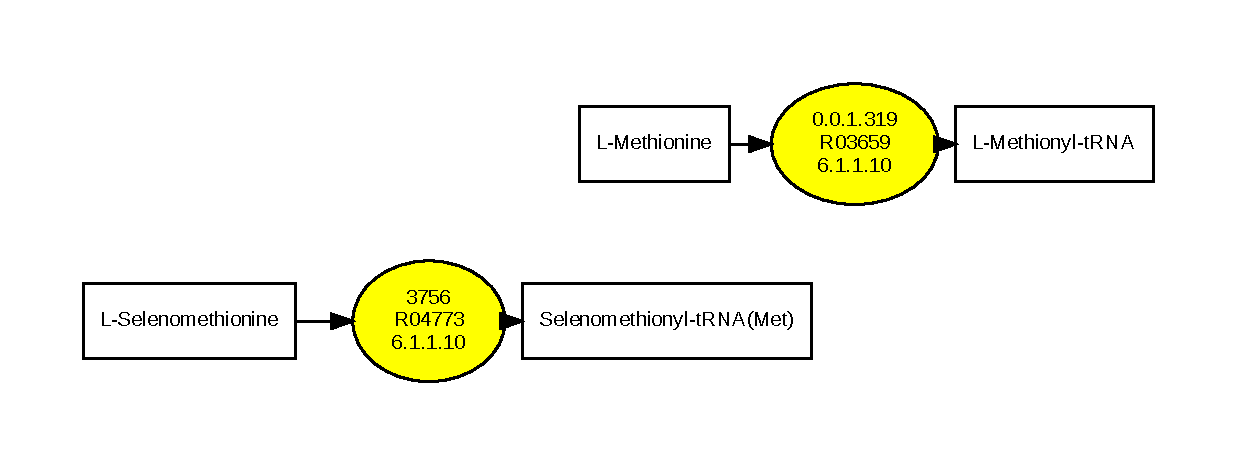
\includegraphics[width=1\textwidth,height=\textheight]{data/0a845f74-826e-3b46-aed9-e7ecf74db262/Groups/MSA_Cluster_3/core/MSA_Cluster_3_core_RC.pdf}

}

\caption{Algae core reaction graph}

\end{figure}%

The global core m-DAG, i.e., the core of all organisms in this example
is empty.

\begin{Shaded}
\begin{Highlighting}[]
\NormalTok{graph\_core\_mDAG}\OtherTok{=}\FunctionTok{read.graph}\NormalTok{(}
  \FunctionTok{paste0}\NormalTok{(path\_exp,}\StringTok{"Global/core/core\_mDAG.graphml"}\NormalTok{),}
  \AttributeTok{format =} \StringTok{"graphml"}\NormalTok{)}
\FunctionTok{summary}\NormalTok{(graph\_core\_mDAG)}
\end{Highlighting}
\end{Shaded}

\begin{verbatim}
IGRAPH 1d0231c D--- 0 0 -- 
+ attr: color (v/c), label (v/c), id (v/c)
\end{verbatim}

The global core m-DAG has 0 vertex and 0 edges. It is an empty graph.

The core metabolic DAG for the Algae group is:

\begin{Shaded}
\begin{Highlighting}[]
\NormalTok{knitr}\SpecialCharTok{::}\FunctionTok{include\_graphics}\NormalTok{(}\FunctionTok{paste0}\NormalTok{(path\_exp,                              }\StringTok{"Groups/Algae/core/Algae\_core\_mDAG.pdf"}\NormalTok{))}
\end{Highlighting}
\end{Shaded}

\begin{figure}[H]

{\centering \includegraphics[width=1\textwidth,height=\textheight]{data/0a845f74-826e-3b46-aed9-e7ecf74db262/Groups/Algae/core/Algae_core_mDAG.pdf}

}

\caption{Core m-DAG for Algae}

\end{figure}%

The global pan reaction graph for the Animals Kingdom is:

\begin{Shaded}
\begin{Highlighting}[]
\NormalTok{graph\_pan\_RC}\OtherTok{=}\FunctionTok{read.graph}\NormalTok{(}
  \FunctionTok{paste0}\NormalTok{(path\_exp,}
         \StringTok{"TaxonomyLevels/Kingdom/Animals/pan/Animals\_pan\_RC.graphml"}\NormalTok{),}
  \AttributeTok{format =} \StringTok{"graphml"}\NormalTok{)}
\FunctionTok{summary}\NormalTok{(graph\_pan\_RC)}
\end{Highlighting}
\end{Shaded}

\begin{verbatim}
IGRAPH 1d12675 D--- 4556 5798 -- 
+ attr: color (v/c), label (v/c), id (v/c), id (e/c)
\end{verbatim}

This pan reaction graph has 4556 nodes and 5798 edges.

\section{Graph's topology}\label{graphs-topology}

From the GraphML files, one can extract topological information. Some
examples are as follows.

The diagram below illustrates the distribution of node degrees for an
m-DAG.

\begin{Shaded}
\begin{Highlighting}[]
\NormalTok{graph\_mDAG}\OtherTok{=}\FunctionTok{read.graph}\NormalTok{(}
  \FunctionTok{paste0}\NormalTok{(path\_exp,}
         \StringTok{"Individuals/hsa/hsa\_mDAG.graphml"}\NormalTok{),}
  \AttributeTok{format=} \StringTok{"graphml"}\NormalTok{)}
\FunctionTok{summary}\NormalTok{(graph\_mDAG)}
\end{Highlighting}
\end{Shaded}

\begin{verbatim}
IGRAPH 1d14d00 D--- 1026 1086 -- 
+ attr: color (v/c), label (v/c), id (v/c), id (e/c)
\end{verbatim}

\begin{Shaded}
\begin{Highlighting}[]
\FunctionTok{barplot}\NormalTok{(}\FunctionTok{table}\NormalTok{(igraph}\SpecialCharTok{::}\FunctionTok{degree}\NormalTok{(graph\_mDAG,}\AttributeTok{mode=}\StringTok{"all"}\NormalTok{)),}
        \AttributeTok{ylim=}\FunctionTok{c}\NormalTok{(}\DecValTok{0}\NormalTok{,}\DecValTok{350}\NormalTok{),}\AttributeTok{col=}\StringTok{"blue"}\NormalTok{,}
        \AttributeTok{main=}\StringTok{"Frequency of Node Degrees"}\NormalTok{,}
        \AttributeTok{ylab=}\StringTok{"Frequency"}\NormalTok{,}\AttributeTok{xlab=}\StringTok{"Degree"}\NormalTok{)}
\end{Highlighting}
\end{Shaded}

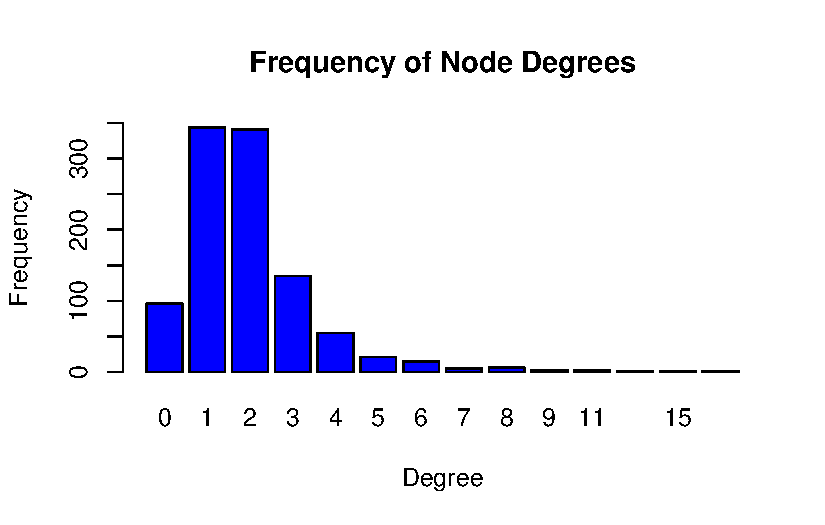
\includegraphics[width=1\textwidth,height=\textheight]{metabolic_graphs_files/figure-pdf/unnamed-chunk-10-1.pdf}

The connected components of every graph as well as the size of every
connected component can be obtained as:

\begin{Shaded}
\begin{Highlighting}[]
\NormalTok{compo}\OtherTok{=}\FunctionTok{components}\NormalTok{(graph\_mDAG,}\AttributeTok{mode =} \StringTok{"weak"}\NormalTok{)}
\FunctionTok{str}\NormalTok{(compo)}
\end{Highlighting}
\end{Shaded}

\begin{verbatim}
List of 3
 $ membership: num [1:1026] 1 1 1 1 1 1 1 1 1 1 ...
 $ csize     : num [1:167] 589 1 1 1 1 1 4 3 4 3 ...
 $ no        : num 167
\end{verbatim}

\begin{Shaded}
\begin{Highlighting}[]
\NormalTok{compo}\SpecialCharTok{$}\NormalTok{csize}
\end{Highlighting}
\end{Shaded}

\begin{verbatim}
  [1] 589   1   1   1   1   1   4   3   4   3   2   3   3   1   1   1   2   6
 [19]   3   1   3   6   1   1   1   1   1   3   1   6   2   1   1   1   2   1
 [37]   1  14   1  16   1   6   2   2   4   1   1   1   1   1   1   1   1   1
 [55]  13   1   1   1   1   2   6   5   5   2   2  10   1   1   1   2   2   1
 [73]   1   1  62   6   2   1   2   1   1   1   2   1   2  14   3   1   1   1
 [91]   1   1   1   1   1   1   3   6   1   3   1   3   2   1   1   1   2   2
[109]   3   1   1   2   5   1   1   2   3   2   1   1   2   3   4   1   1   2
[127]   1   1   2   1   1   1   1   1   3   1   2   2   1   6   1   1   1   2
[145]   1   1   1   1   1   2   7   1  15   3   1   1   1   1   2   1   3   1
[163]   1   1   1   1   2
\end{verbatim}

\begin{Shaded}
\begin{Highlighting}[]
\NormalTok{k}\OtherTok{=}\FunctionTok{which.max}\NormalTok{(compo}\SpecialCharTok{$}\NormalTok{csize}\SpecialCharTok{==}\FunctionTok{max}\NormalTok{(compo}\SpecialCharTok{$}\NormalTok{csize))}
\NormalTok{k}
\end{Highlighting}
\end{Shaded}

\begin{verbatim}
[1] 1
\end{verbatim}

\begin{Shaded}
\begin{Highlighting}[]
\FunctionTok{table}\NormalTok{(compo}\SpecialCharTok{$}\NormalTok{membership)}
\end{Highlighting}
\end{Shaded}

\begin{verbatim}

  1   2   3   4   5   6   7   8   9  10  11  12  13  14  15  16  17  18  19  20 
589   1   1   1   1   1   4   3   4   3   2   3   3   1   1   1   2   6   3   1 
 21  22  23  24  25  26  27  28  29  30  31  32  33  34  35  36  37  38  39  40 
  3   6   1   1   1   1   1   3   1   6   2   1   1   1   2   1   1  14   1  16 
 41  42  43  44  45  46  47  48  49  50  51  52  53  54  55  56  57  58  59  60 
  1   6   2   2   4   1   1   1   1   1   1   1   1   1  13   1   1   1   1   2 
 61  62  63  64  65  66  67  68  69  70  71  72  73  74  75  76  77  78  79  80 
  6   5   5   2   2  10   1   1   1   2   2   1   1   1  62   6   2   1   2   1 
 81  82  83  84  85  86  87  88  89  90  91  92  93  94  95  96  97  98  99 100 
  1   1   2   1   2  14   3   1   1   1   1   1   1   1   1   1   3   6   1   3 
101 102 103 104 105 106 107 108 109 110 111 112 113 114 115 116 117 118 119 120 
  1   3   2   1   1   1   2   2   3   1   1   2   5   1   1   2   3   2   1   1 
121 122 123 124 125 126 127 128 129 130 131 132 133 134 135 136 137 138 139 140 
  2   3   4   1   1   2   1   1   2   1   1   1   1   1   3   1   2   2   1   6 
141 142 143 144 145 146 147 148 149 150 151 152 153 154 155 156 157 158 159 160 
  1   1   1   2   1   1   1   1   1   2   7   1  15   3   1   1   1   1   2   1 
161 162 163 164 165 166 167 
  3   1   1   1   1   1   2 
\end{verbatim}

\begin{Shaded}
\begin{Highlighting}[]
\NormalTok{vertex}\OtherTok{=}\FunctionTok{which}\NormalTok{(compo}\SpecialCharTok{$}\NormalTok{membership}\SpecialCharTok{==}\NormalTok{k)}
\FunctionTok{length}\NormalTok{(vertex)}
\end{Highlighting}
\end{Shaded}

\begin{verbatim}
[1] 589
\end{verbatim}

\begin{Shaded}
\begin{Highlighting}[]
\NormalTok{Big\_Component}\OtherTok{=}\FunctionTok{induced\_subgraph}\NormalTok{(graph\_mDAG, }\AttributeTok{vids=}\NormalTok{vertex)}
\NormalTok{igraph}\SpecialCharTok{::}\FunctionTok{vcount}\NormalTok{(Big\_Component)}
\end{Highlighting}
\end{Shaded}

\begin{verbatim}
[1] 589
\end{verbatim}

\begin{Shaded}
\begin{Highlighting}[]
\NormalTok{igraph}\SpecialCharTok{::}\FunctionTok{ecount}\NormalTok{(Big\_Component)}
\end{Highlighting}
\end{Shaded}

\begin{verbatim}
[1] 774
\end{verbatim}

And the plot of the bigger component of the m-DAG in Homo sapiens is:

\begin{Shaded}
\begin{Highlighting}[]
\NormalTok{knitr}\SpecialCharTok{::}\FunctionTok{include\_graphics}\NormalTok{(}\FunctionTok{paste0}\NormalTok{(path\_exp,}
                               \StringTok{"Individuals/hsa/hsa\_mDAG\_biggerDAG.pdf"}\NormalTok{))}
\end{Highlighting}
\end{Shaded}

\begin{center}
\includegraphics[width=1\textwidth,height=\textheight]{data/0a845f74-826e-3b46-aed9-e7ecf74db262/Individuals/hsa/hsa_mDAG_biggerDAG.pdf}
\end{center}

\begin{Shaded}
\begin{Highlighting}[]
\CommentTok{\#path\_exp="data/result\_bb261b6e{-}95c6{-}3e39{-}b82b{-}b68eea80e30b/data/" }
\NormalTok{list\_names}\OtherTok{=}\FunctionTok{dir}\NormalTok{(}\FunctionTok{paste0}\NormalTok{(path\_exp,}\StringTok{"Individuals/"}\NormalTok{))}
\NormalTok{list\_names}\OtherTok{=}\NormalTok{ list\_names[}\SpecialCharTok{{-}}\DecValTok{1}\NormalTok{] }\CommentTok{\# filter 0000\_RefPw}
\FunctionTok{length}\NormalTok{(list\_names) }
\end{Highlighting}
\end{Shaded}

\begin{verbatim}
[1] 884
\end{verbatim}

\begin{Shaded}
\begin{Highlighting}[]
\NormalTok{graphs\_list}\OtherTok{=}\FunctionTok{paste0}\NormalTok{(path\_exp,}\StringTok{"Individuals/"}\NormalTok{, list\_names,}\StringTok{"/"}\NormalTok{,list\_names, }\StringTok{"\_MDAG.graphml"}\NormalTok{)}
\end{Highlighting}
\end{Shaded}

\begin{Shaded}
\begin{Highlighting}[]
\NormalTok{knitr}\SpecialCharTok{::}\FunctionTok{include\_graphics}\NormalTok{(}
  \FunctionTok{paste0}\NormalTok{(path\_exp,}\StringTok{"Individuals/cang/cang\_RC.pdf"}\NormalTok{))}
\end{Highlighting}
\end{Shaded}

\includegraphics[width=1\textwidth,height=\textheight]{data/0a845f74-826e-3b46-aed9-e7ecf74db262/Individuals/cang/cang_RC.pdf}

\section{Graph statistics}\label{graph-statistics}

The number of connected component in each generated m-DAG with their
frequency in the entire set of m-DAGs, can be obtained as follows:

\begin{Shaded}
\begin{Highlighting}[]
\NormalTok{read\_mDAG}\OtherTok{=}\ControlFlowTok{function}\NormalTok{(x) \{DAG}\OtherTok{=}\FunctionTok{read.graph}\NormalTok{(}\AttributeTok{file=}\NormalTok{x,}
                                      \AttributeTok{format=}\StringTok{"graphml"}\NormalTok{)}
\FunctionTok{return}\NormalTok{(DAG)\}}
\NormalTok{mDAG\_componets}\OtherTok{=}\ControlFlowTok{function}\NormalTok{(x) \{}
  \FunctionTok{sort}\NormalTok{(}\FunctionTok{components}\NormalTok{(x,}\AttributeTok{mode =} \StringTok{"weak"}\NormalTok{)}\SpecialCharTok{$}\NormalTok{csize,}
       \AttributeTok{decreasing=}\ConstantTok{TRUE}\NormalTok{)}
\NormalTok{\}}

\NormalTok{compo\_list}\OtherTok{=}\FunctionTok{lapply}\NormalTok{(graphs\_list,}
                  \AttributeTok{FUN=}\ControlFlowTok{function}\NormalTok{(x) \{}
\NormalTok{                    gg}\OtherTok{=}\FunctionTok{read\_mDAG}\NormalTok{(x)}
\NormalTok{                    aux}\OtherTok{=}\FunctionTok{list}\NormalTok{(}
                      \AttributeTok{mDAG\_componets=}\FunctionTok{mDAG\_componets}\NormalTok{(gg),}
                      \AttributeTok{degree\_count=}\NormalTok{igraph}\SpecialCharTok{::}\FunctionTok{degree}\NormalTok{(gg,}\AttributeTok{mode=}\StringTok{"total"}\NormalTok{))}
                    \FunctionTok{return}\NormalTok{(aux)\}}
\NormalTok{)}

\FunctionTok{names}\NormalTok{(compo\_list)}\OtherTok{=}\NormalTok{list\_names}
\NormalTok{n}\OtherTok{=}\FunctionTok{max}\NormalTok{(}\FunctionTok{sapply}\NormalTok{(compo\_list,}\AttributeTok{FUN=}\ControlFlowTok{function}\NormalTok{(x) \{}\FunctionTok{length}\NormalTok{(x[[}\DecValTok{1}\NormalTok{]])\}))}
\NormalTok{n}
\end{Highlighting}
\end{Shaded}

\begin{verbatim}
[1] 234
\end{verbatim}

\begin{Shaded}
\begin{Highlighting}[]
\NormalTok{size\_compo\_list}\OtherTok{=}\FunctionTok{lapply}\NormalTok{(compo\_list,}\AttributeTok{FUN=}\ControlFlowTok{function}\NormalTok{(x) \{}
  \FunctionTok{return}\NormalTok{(}\FunctionTok{c}\NormalTok{(x[[}\DecValTok{1}\NormalTok{]],}\FunctionTok{rep}\NormalTok{(}\ConstantTok{NA}\NormalTok{,n}\SpecialCharTok{{-}}\FunctionTok{length}\NormalTok{(x[[}\DecValTok{1}\NormalTok{]]))))\})}

\NormalTok{aux}\OtherTok{=}\FunctionTok{do.call}\NormalTok{(bind\_cols,size\_compo\_list)}
\NormalTok{weak\_componets\_size}\OtherTok{=}\FunctionTok{pivot\_longer}\NormalTok{(aux,aaf}\SpecialCharTok{:}\NormalTok{zvi,}\AttributeTok{names\_to=}\StringTok{"Organism"}\NormalTok{,}
                                 \AttributeTok{values\_to=}\StringTok{"csize"}\NormalTok{) }\SpecialCharTok{\%\textgreater{}\%}
  \FunctionTok{arrange}\NormalTok{(Organism,}\SpecialCharTok{{-}}\NormalTok{csize)}
\NormalTok{weak\_componets\_size}\SpecialCharTok{$}\NormalTok{index}\OtherTok{=}\FunctionTok{rep}\NormalTok{(}\DecValTok{1}\SpecialCharTok{:}\NormalTok{n,}\AttributeTok{times=}\FunctionTok{dim}\NormalTok{(aux)[}\DecValTok{2}\NormalTok{])}
\NormalTok{weak\_componets\_size}\OtherTok{=}\NormalTok{weak\_componets\_size }\SpecialCharTok{\%\textgreater{}\%}
  \FunctionTok{left\_join}\NormalTok{(meta\_taxo,}\AttributeTok{by=}\StringTok{"Organism"}\NormalTok{) }\SpecialCharTok{\%\textgreater{}\%} \FunctionTok{filter}\NormalTok{(}\SpecialCharTok{!}\FunctionTok{is.na}\NormalTok{(Kingdom),}\SpecialCharTok{!}\FunctionTok{is.na}\NormalTok{(csize))}
\end{Highlighting}
\end{Shaded}

\begin{Shaded}
\begin{Highlighting}[]
\NormalTok{Organism}\OtherTok{=}\FunctionTok{names}\NormalTok{(compo\_list)}
\NormalTok{big\_MBB}\OtherTok{=}\ControlFlowTok{function}\NormalTok{(org)\{}
\NormalTok{  org}\OtherTok{=}\StringTok{"hsa"}
\NormalTok{  x}\OtherTok{=}\NormalTok{Results }\SpecialCharTok{\%\textgreater{}\%} \FunctionTok{filter}\NormalTok{(Organism}\SpecialCharTok{==}\NormalTok{org)}
\NormalTok{  x}\OtherTok{=}\FunctionTok{as.character}\NormalTok{(x[}\DecValTok{1}\NormalTok{,}\DecValTok{5}\SpecialCharTok{:}\FunctionTok{dim}\NormalTok{(Results)[}\DecValTok{2}\NormalTok{]])}
\NormalTok{  x}\OtherTok{=}\NormalTok{x[x}\SpecialCharTok{!=}\StringTok{"NA"}\NormalTok{]}
\NormalTok{  tt}\OtherTok{=}\FunctionTok{sort}\NormalTok{(}\FunctionTok{table}\NormalTok{(x),}\AttributeTok{decreasing=}\ConstantTok{TRUE}\NormalTok{)}
  \FunctionTok{return}\NormalTok{(tt)}
\NormalTok{\}}
\NormalTok{big\_MBB\_list}\OtherTok{=} \FunctionTok{lapply}\NormalTok{(Organism,}\AttributeTok{FUN=}\ControlFlowTok{function}\NormalTok{(x) }\FunctionTok{big\_MBB}\NormalTok{(x))}
\NormalTok{nMBB}\OtherTok{=}\FunctionTok{max}\NormalTok{(}\FunctionTok{sapply}\NormalTok{(big\_MBB\_list,}\AttributeTok{FUN=}\ControlFlowTok{function}\NormalTok{(x) }\FunctionTok{length}\NormalTok{(x)))}
\NormalTok{nMBB}
\end{Highlighting}
\end{Shaded}

\begin{verbatim}
[1] 1028
\end{verbatim}

\begin{Shaded}
\begin{Highlighting}[]
\NormalTok{big\_MBB\_list}\OtherTok{=}\FunctionTok{lapply}\NormalTok{(big\_MBB\_list,}
                    \AttributeTok{FUN=}\ControlFlowTok{function}\NormalTok{(x)\{}
\NormalTok{                      x}\OtherTok{=}\FunctionTok{c}\NormalTok{(x,}\FunctionTok{rep}\NormalTok{(}\ConstantTok{NA}\NormalTok{,nMBB}\SpecialCharTok{{-}}\FunctionTok{length}\NormalTok{(x)))}
                      \FunctionTok{return}\NormalTok{(x)\}}
\NormalTok{)}
\FunctionTok{names}\NormalTok{(big\_MBB\_list)}\OtherTok{=}\NormalTok{Organism}
\NormalTok{big\_MBB\_list}\OtherTok{=}\FunctionTok{do.call}\NormalTok{(bind\_cols,big\_MBB\_list)}

\NormalTok{kMBB}\OtherTok{=}\FunctionTok{nrow}\NormalTok{(big\_MBB\_list)}
\NormalTok{index}\OtherTok{=}\FunctionTok{rep}\NormalTok{(}\DecValTok{1}\SpecialCharTok{:}\NormalTok{kMBB,}\AttributeTok{times=}\FunctionTok{length}\NormalTok{(Organism))}


\NormalTok{big\_MBB\_list2}\OtherTok{=}\FunctionTok{pivot\_longer}\NormalTok{(big\_MBB\_list,}
                           \AttributeTok{cols=}\FunctionTok{names}\NormalTok{(big\_MBB\_list),}
                           \AttributeTok{values\_to =} \StringTok{"MBBsize"}\NormalTok{,}
                           \AttributeTok{names\_to =} \StringTok{"Organism"}\NormalTok{) }\SpecialCharTok{\%\textgreater{}\%} 
  \FunctionTok{arrange}\NormalTok{(Organism,}\SpecialCharTok{{-}}\NormalTok{MBBsize) }\SpecialCharTok{\%\textgreater{}\%}  
  \FunctionTok{mutate}\NormalTok{(}\AttributeTok{index=}\NormalTok{index) }\SpecialCharTok{\%\textgreater{}\%} 
  \FunctionTok{left\_join}\NormalTok{(meta\_taxo,}\AttributeTok{by=}\StringTok{"Organism"}\NormalTok{)}
\end{Highlighting}
\end{Shaded}

We can visualize the sizes of the weak components for each m-DAG, using
colors to represent the different Kingdoms, also we scale the results by
a log-log plot:

\begin{Shaded}
\begin{Highlighting}[]
\NormalTok{COLOR\_KINGDOM}\OtherTok{=}\FunctionTok{c}\NormalTok{(}\StringTok{"red"}\NormalTok{,}\StringTok{"yellow"}\NormalTok{,}\StringTok{"green"}\NormalTok{,}\StringTok{"black"}\NormalTok{)}
\NormalTok{colors\_kingdom}\OtherTok{=}\NormalTok{weak\_componets\_size}\SpecialCharTok{\%\textgreater{}\%} \FunctionTok{select}\NormalTok{(Organism,Kingdom) }\SpecialCharTok{\%\textgreater{}\%} \FunctionTok{distinct}\NormalTok{()}
\FunctionTok{names}\NormalTok{(COLOR\_KINGDOM)}\OtherTok{=}\FunctionTok{sort}\NormalTok{(}\FunctionTok{unique}\NormalTok{(colors\_kingdom}\SpecialCharTok{$}\NormalTok{Kingdom))}

\NormalTok{p1}\OtherTok{\textless{}{-}} \FunctionTok{ggplot}\NormalTok{(}\AttributeTok{data=}\NormalTok{weak\_componets\_size) }\SpecialCharTok{+} 
  \FunctionTok{geom\_line}\NormalTok{(}\AttributeTok{mapping=}\FunctionTok{aes}\NormalTok{(}\AttributeTok{x=}\NormalTok{index,}
                        \AttributeTok{y=}\NormalTok{csize,}\AttributeTok{group =}\NormalTok{ Organism,}
                        \AttributeTok{color=}\NormalTok{Kingdom),}
            \AttributeTok{na.rm=}\ConstantTok{TRUE}\NormalTok{) }\SpecialCharTok{+} 
  \FunctionTok{scale\_x\_continuous}\NormalTok{(}\AttributeTok{trans=}\StringTok{"identity"}\NormalTok{) }\SpecialCharTok{+} 
  \FunctionTok{scale\_y\_continuous}\NormalTok{(}\AttributeTok{trans=}\StringTok{"identity"}\NormalTok{) }\SpecialCharTok{+}
  \FunctionTok{ylim}\NormalTok{(}\DecValTok{0}\NormalTok{,}\DecValTok{640}\NormalTok{)}\SpecialCharTok{+}
  \FunctionTok{ggtitle}\NormalTok{(}\StringTok{"Plot of weak components size decreasing order."}\NormalTok{)}\SpecialCharTok{+}
  \FunctionTok{ylab}\NormalTok{(}\StringTok{"Weak components size"}\NormalTok{) }\SpecialCharTok{+} \FunctionTok{xlab}\NormalTok{(}\StringTok{"Order"}\NormalTok{)}\SpecialCharTok{+}
  \FunctionTok{scale\_color\_manual}\NormalTok{(}\AttributeTok{values =}\NormalTok{COLOR\_KINGDOM[colors\_kingdom}\SpecialCharTok{$}\NormalTok{Kingdom])}

\NormalTok{p2}\OtherTok{\textless{}{-}} \FunctionTok{ggplot}\NormalTok{(}\AttributeTok{data=}\NormalTok{weak\_componets\_size) }\SpecialCharTok{+} 
  \FunctionTok{geom\_line}\NormalTok{(}\AttributeTok{mapping=}\FunctionTok{aes}\NormalTok{(}\AttributeTok{x=}\NormalTok{index,}
                        \AttributeTok{y=}\NormalTok{csize,}\AttributeTok{group =}\NormalTok{ Organism,}
                        \AttributeTok{color=}\NormalTok{Kingdom),}
            \AttributeTok{na.rm=}\ConstantTok{TRUE}\NormalTok{) }\SpecialCharTok{+} 
  \FunctionTok{scale\_y\_continuous}\NormalTok{(}\AttributeTok{trans=}\StringTok{\textquotesingle{}log10\textquotesingle{}}\NormalTok{) }\SpecialCharTok{+} 
  \FunctionTok{scale\_x\_continuous}\NormalTok{(}\AttributeTok{trans=}\StringTok{\textquotesingle{}log10\textquotesingle{}}\NormalTok{) }\SpecialCharTok{+}
  \FunctionTok{scale\_color\_manual}\NormalTok{(}\AttributeTok{values =}\NormalTok{COLOR\_KINGDOM[colors\_kingdom}\SpecialCharTok{$}\NormalTok{Kingdom])}\SpecialCharTok{+}
  \FunctionTok{ggtitle}\NormalTok{(}\StringTok{"Plot log10{-}log10 of size  weak components decreasing order."}\NormalTok{) }\SpecialCharTok{+}
  \FunctionTok{ylab}\NormalTok{(}\StringTok{"Log10 weak component size"}\NormalTok{) }\SpecialCharTok{+} \FunctionTok{xlab}\NormalTok{(}\StringTok{"Log10 order"}\NormalTok{)}
\NormalTok{p1}
\end{Highlighting}
\end{Shaded}

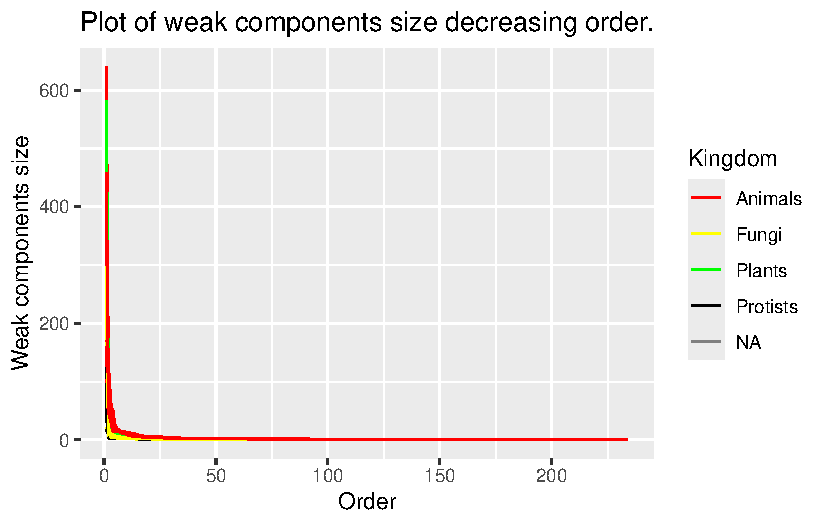
\includegraphics[width=1\textwidth,height=\textheight]{metabolic_graphs_files/figure-pdf/unnamed-chunk-17-1.pdf}

\begin{Shaded}
\begin{Highlighting}[]
\NormalTok{p2}
\end{Highlighting}
\end{Shaded}

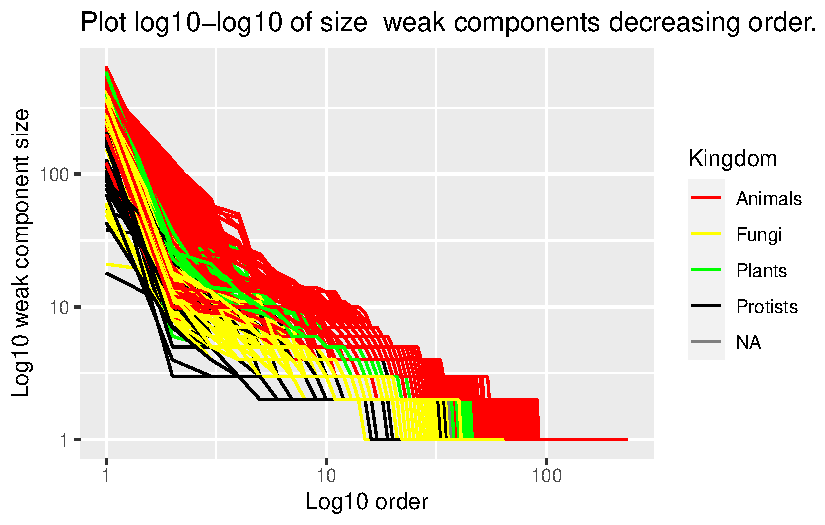
\includegraphics[width=1\textwidth,height=\textheight]{metabolic_graphs_files/figure-pdf/unnamed-chunk-17-2.pdf}

A table with the frequencies of the weak connected components sizes,
displayed by Kingdom, can be obtained as follows:

\begin{Shaded}
\begin{Highlighting}[]
\NormalTok{aux}\OtherTok{=}\FunctionTok{table}\NormalTok{(weak\_componets\_size}\SpecialCharTok{$}\NormalTok{csize,weak\_componets\_size}\SpecialCharTok{$}\NormalTok{Kingdom)}
\NormalTok{table\_wcc\_size}\OtherTok{=}\FunctionTok{tibble}\NormalTok{(}\AttributeTok{Order=}\DecValTok{1}\SpecialCharTok{:}\FunctionTok{dim}\NormalTok{(aux)[}\DecValTok{1}\NormalTok{],}
                      \AttributeTok{Wcc\_size=}\FunctionTok{as.integer}\NormalTok{(}\FunctionTok{unlist}\NormalTok{(}\FunctionTok{dimnames}\NormalTok{(aux)[}\DecValTok{1}\NormalTok{])),}
                      \AttributeTok{Animals=}\NormalTok{aux[,}\DecValTok{1}\NormalTok{],}
                      \AttributeTok{Fungi=}\NormalTok{aux[,}\DecValTok{2}\NormalTok{],}
                      \AttributeTok{Plants=}\NormalTok{aux[,}\DecValTok{3}\NormalTok{],}
                      \AttributeTok{Protists=}\NormalTok{aux[,}\DecValTok{4}\NormalTok{])}
\NormalTok{knitr}\SpecialCharTok{::}\FunctionTok{kable}\NormalTok{(table\_wcc\_size)}
\end{Highlighting}
\end{Shaded}

\begin{longtable}[]{@{}rrrrrr@{}}
\toprule\noalign{}
Order & Wcc\_size & Animals & Fungi & Plants & Protists \\
\midrule\noalign{}
\endhead
\bottomrule\noalign{}
\endlastfoot
1 & 1 & 57634 & 15311 & 15024 & 4462 \\
2 & 2 & 13528 & 2118 & 2908 & 932 \\
3 & 3 & 7018 & 1070 & 911 & 317 \\
4 & 4 & 2459 & 313 & 292 & 96 \\
5 & 5 & 1962 & 215 & 389 & 81 \\
6 & 6 & 1778 & 154 & 323 & 49 \\
7 & 7 & 633 & 46 & 111 & 15 \\
8 & 8 & 278 & 57 & 110 & 7 \\
9 & 9 & 174 & 76 & 151 & 22 \\
10 & 10 & 671 & 6 & 124 & 7 \\
11 & 11 & 411 & 14 & 6 & 20 \\
12 & 12 & 109 & 12 & 4 & 5 \\
13 & 13 & 369 & 92 & 132 & 7 \\
14 & 14 & 774 & 9 & 2 & 2 \\
15 & 15 & 234 & 1 & 5 & 6 \\
16 & 16 & 79 & 6 & 1 & 1 \\
17 & 17 & 55 & 8 & 1 & 1 \\
18 & 18 & 4 & 5 & 9 & 5 \\
19 & 19 & 5 & 3 & 87 & 4 \\
20 & 20 & 9 & 3 & 0 & 1 \\
21 & 21 & 13 & 2 & 12 & 1 \\
22 & 22 & 7 & 2 & 2 & 0 \\
23 & 23 & 21 & 1 & 3 & 0 \\
24 & 24 & 19 & 1 & 3 & 1 \\
25 & 25 & 20 & 0 & 2 & 1 \\
26 & 26 & 12 & 0 & 39 & 0 \\
27 & 27 & 1 & 1 & 11 & 0 \\
28 & 28 & 5 & 2 & 77 & 0 \\
29 & 29 & 40 & 1 & 0 & 1 \\
30 & 30 & 0 & 1 & 1 & 0 \\
31 & 31 & 72 & 8 & 1 & 0 \\
32 & 32 & 11 & 7 & 1 & 0 \\
33 & 33 & 1 & 0 & 0 & 2 \\
34 & 34 & 6 & 0 & 0 & 0 \\
35 & 35 & 2 & 0 & 0 & 0 \\
36 & 36 & 3 & 0 & 0 & 0 \\
37 & 37 & 5 & 1 & 2 & 0 \\
38 & 38 & 0 & 0 & 0 & 1 \\
39 & 39 & 5 & 0 & 0 & 0 \\
40 & 40 & 5 & 1 & 0 & 0 \\
41 & 41 & 4 & 0 & 0 & 0 \\
42 & 42 & 1 & 0 & 0 & 0 \\
43 & 43 & 2 & 0 & 0 & 1 \\
44 & 44 & 6 & 0 & 0 & 0 \\
45 & 45 & 1 & 0 & 0 & 0 \\
46 & 46 & 5 & 0 & 0 & 0 \\
47 & 47 & 9 & 0 & 0 & 0 \\
48 & 48 & 1 & 0 & 0 & 0 \\
49 & 49 & 1 & 1 & 0 & 0 \\
50 & 50 & 1 & 0 & 0 & 0 \\
51 & 51 & 4 & 0 & 0 & 0 \\
52 & 53 & 50 & 1 & 0 & 1 \\
53 & 54 & 6 & 0 & 0 & 0 \\
54 & 55 & 1 & 0 & 0 & 0 \\
55 & 56 & 8 & 0 & 0 & 0 \\
56 & 57 & 2 & 0 & 0 & 0 \\
57 & 58 & 12 & 1 & 0 & 0 \\
58 & 59 & 6 & 0 & 0 & 0 \\
59 & 60 & 30 & 1 & 0 & 0 \\
60 & 61 & 5 & 0 & 0 & 0 \\
61 & 62 & 15 & 0 & 0 & 0 \\
62 & 63 & 4 & 0 & 0 & 0 \\
63 & 64 & 2 & 0 & 0 & 0 \\
64 & 65 & 34 & 0 & 0 & 0 \\
65 & 66 & 6 & 0 & 0 & 0 \\
66 & 67 & 1 & 0 & 0 & 0 \\
67 & 69 & 1 & 0 & 0 & 0 \\
68 & 70 & 2 & 0 & 0 & 1 \\
69 & 71 & 1 & 0 & 0 & 0 \\
70 & 72 & 1 & 0 & 0 & 0 \\
71 & 73 & 6 & 0 & 0 & 0 \\
72 & 77 & 2 & 0 & 0 & 1 \\
73 & 78 & 1 & 0 & 0 & 1 \\
74 & 83 & 0 & 0 & 0 & 2 \\
75 & 84 & 1 & 0 & 0 & 0 \\
76 & 87 & 1 & 0 & 0 & 0 \\
77 & 88 & 1 & 0 & 0 & 1 \\
78 & 90 & 2 & 0 & 0 & 1 \\
79 & 91 & 1 & 0 & 0 & 0 \\
80 & 94 & 4 & 0 & 0 & 1 \\
81 & 95 & 1 & 0 & 0 & 0 \\
82 & 96 & 1 & 0 & 0 & 1 \\
83 & 97 & 0 & 0 & 0 & 1 \\
84 & 99 & 1 & 0 & 0 & 1 \\
85 & 100 & 2 & 0 & 0 & 0 \\
86 & 101 & 1 & 0 & 0 & 0 \\
87 & 102 & 0 & 0 & 0 & 1 \\
88 & 103 & 3 & 0 & 0 & 1 \\
89 & 104 & 0 & 0 & 0 & 2 \\
90 & 105 & 0 & 0 & 0 & 1 \\
91 & 107 & 0 & 0 & 0 & 1 \\
92 & 108 & 1 & 0 & 0 & 2 \\
93 & 110 & 2 & 0 & 0 & 0 \\
94 & 111 & 1 & 0 & 0 & 0 \\
95 & 112 & 0 & 1 & 0 & 0 \\
96 & 113 & 2 & 0 & 0 & 0 \\
97 & 114 & 1 & 0 & 0 & 1 \\
98 & 116 & 1 & 0 & 0 & 0 \\
99 & 117 & 3 & 0 & 0 & 0 \\
100 & 120 & 1 & 0 & 0 & 0 \\
101 & 121 & 2 & 0 & 0 & 0 \\
102 & 125 & 1 & 0 & 0 & 0 \\
103 & 127 & 1 & 0 & 0 & 1 \\
104 & 128 & 0 & 0 & 0 & 2 \\
105 & 153 & 0 & 1 & 0 & 0 \\
106 & 166 & 0 & 0 & 0 & 1 \\
107 & 175 & 0 & 0 & 0 & 2 \\
108 & 181 & 0 & 0 & 0 & 1 \\
109 & 183 & 0 & 0 & 0 & 2 \\
110 & 184 & 1 & 0 & 0 & 0 \\
111 & 187 & 0 & 0 & 0 & 1 \\
112 & 193 & 1 & 0 & 0 & 1 \\
113 & 195 & 0 & 0 & 0 & 1 \\
114 & 196 & 0 & 0 & 0 & 1 \\
115 & 198 & 1 & 0 & 0 & 0 \\
116 & 203 & 0 & 0 & 0 & 1 \\
117 & 205 & 0 & 0 & 0 & 1 \\
118 & 210 & 2 & 0 & 0 & 0 \\
119 & 219 & 1 & 0 & 0 & 1 \\
120 & 220 & 1 & 0 & 0 & 0 \\
121 & 229 & 1 & 0 & 0 & 0 \\
122 & 231 & 0 & 0 & 0 & 1 \\
123 & 232 & 1 & 0 & 0 & 0 \\
124 & 233 & 0 & 1 & 0 & 0 \\
125 & 235 & 1 & 0 & 0 & 0 \\
126 & 238 & 3 & 0 & 0 & 0 \\
127 & 243 & 1 & 0 & 0 & 0 \\
128 & 245 & 0 & 1 & 0 & 0 \\
129 & 246 & 1 & 1 & 0 & 0 \\
130 & 248 & 0 & 1 & 0 & 0 \\
131 & 249 & 0 & 2 & 0 & 0 \\
132 & 250 & 0 & 2 & 0 & 0 \\
133 & 251 & 0 & 1 & 0 & 0 \\
134 & 252 & 1 & 2 & 0 & 0 \\
135 & 253 & 1 & 0 & 0 & 0 \\
136 & 254 & 0 & 1 & 0 & 0 \\
137 & 255 & 2 & 0 & 0 & 0 \\
138 & 256 & 2 & 1 & 0 & 0 \\
139 & 257 & 4 & 0 & 0 & 0 \\
140 & 258 & 1 & 1 & 0 & 0 \\
141 & 259 & 1 & 0 & 0 & 0 \\
142 & 260 & 2 & 1 & 0 & 1 \\
143 & 261 & 2 & 1 & 0 & 0 \\
144 & 262 & 2 & 0 & 0 & 0 \\
145 & 263 & 4 & 1 & 0 & 1 \\
146 & 264 & 4 & 0 & 0 & 0 \\
147 & 265 & 3 & 4 & 0 & 2 \\
148 & 266 & 2 & 1 & 0 & 0 \\
149 & 267 & 2 & 1 & 0 & 0 \\
150 & 268 & 2 & 3 & 0 & 1 \\
151 & 269 & 3 & 1 & 0 & 0 \\
152 & 270 & 3 & 0 & 1 & 0 \\
153 & 271 & 1 & 1 & 0 & 0 \\
154 & 272 & 2 & 2 & 0 & 0 \\
155 & 273 & 4 & 3 & 0 & 1 \\
156 & 274 & 2 & 1 & 0 & 0 \\
157 & 275 & 4 & 2 & 0 & 0 \\
158 & 276 & 0 & 2 & 0 & 0 \\
159 & 277 & 4 & 4 & 0 & 0 \\
160 & 278 & 3 & 3 & 0 & 1 \\
161 & 279 & 5 & 0 & 0 & 1 \\
162 & 280 & 1 & 0 & 0 & 0 \\
163 & 281 & 3 & 4 & 0 & 0 \\
164 & 282 & 4 & 1 & 0 & 0 \\
165 & 283 & 5 & 1 & 0 & 0 \\
166 & 284 & 4 & 1 & 0 & 0 \\
167 & 285 & 5 & 1 & 0 & 0 \\
168 & 286 & 4 & 2 & 0 & 1 \\
169 & 287 & 1 & 0 & 0 & 0 \\
170 & 288 & 2 & 3 & 0 & 0 \\
171 & 289 & 1 & 0 & 0 & 0 \\
172 & 290 & 3 & 0 & 0 & 0 \\
173 & 291 & 1 & 1 & 0 & 0 \\
174 & 292 & 1 & 3 & 0 & 1 \\
175 & 293 & 5 & 1 & 0 & 0 \\
176 & 294 & 6 & 0 & 0 & 0 \\
177 & 295 & 1 & 2 & 0 & 0 \\
178 & 296 & 5 & 1 & 0 & 0 \\
179 & 297 & 4 & 1 & 0 & 0 \\
180 & 298 & 2 & 1 & 0 & 0 \\
181 & 299 & 2 & 0 & 1 & 1 \\
182 & 300 & 2 & 0 & 0 & 0 \\
183 & 301 & 4 & 2 & 0 & 0 \\
184 & 302 & 1 & 0 & 0 & 1 \\
185 & 303 & 3 & 0 & 0 & 0 \\
186 & 304 & 3 & 0 & 0 & 0 \\
187 & 305 & 3 & 0 & 0 & 0 \\
188 & 306 & 2 & 1 & 0 & 0 \\
189 & 307 & 4 & 1 & 0 & 0 \\
190 & 308 & 1 & 0 & 0 & 0 \\
191 & 310 & 1 & 0 & 0 & 0 \\
192 & 311 & 1 & 0 & 1 & 0 \\
193 & 313 & 2 & 2 & 0 & 0 \\
194 & 315 & 1 & 0 & 0 & 0 \\
195 & 316 & 1 & 0 & 0 & 0 \\
196 & 317 & 1 & 0 & 1 & 0 \\
197 & 318 & 0 & 2 & 0 & 0 \\
198 & 319 & 1 & 0 & 0 & 0 \\
199 & 320 & 3 & 1 & 1 & 0 \\
200 & 321 & 1 & 0 & 0 & 0 \\
201 & 322 & 3 & 0 & 0 & 0 \\
202 & 323 & 2 & 0 & 0 & 0 \\
203 & 325 & 1 & 0 & 0 & 0 \\
204 & 327 & 2 & 1 & 0 & 0 \\
205 & 328 & 5 & 1 & 1 & 0 \\
206 & 330 & 0 & 1 & 0 & 0 \\
207 & 332 & 1 & 0 & 0 & 0 \\
208 & 333 & 1 & 1 & 1 & 1 \\
209 & 335 & 1 & 0 & 0 & 0 \\
210 & 338 & 1 & 0 & 0 & 0 \\
211 & 339 & 0 & 0 & 1 & 1 \\
212 & 340 & 1 & 1 & 0 & 0 \\
213 & 341 & 1 & 0 & 0 & 0 \\
214 & 342 & 1 & 0 & 0 & 1 \\
215 & 343 & 2 & 1 & 0 & 0 \\
216 & 344 & 0 & 0 & 1 & 0 \\
217 & 345 & 2 & 0 & 0 & 0 \\
218 & 346 & 1 & 0 & 0 & 0 \\
219 & 347 & 2 & 0 & 0 & 0 \\
220 & 349 & 2 & 0 & 0 & 0 \\
221 & 350 & 1 & 0 & 0 & 0 \\
222 & 351 & 1 & 0 & 0 & 0 \\
223 & 352 & 3 & 0 & 0 & 0 \\
224 & 353 & 1 & 0 & 0 & 0 \\
225 & 354 & 1 & 0 & 0 & 0 \\
226 & 355 & 2 & 0 & 0 & 0 \\
227 & 356 & 1 & 1 & 0 & 0 \\
228 & 357 & 1 & 2 & 0 & 0 \\
229 & 358 & 2 & 1 & 0 & 0 \\
230 & 359 & 0 & 0 & 1 & 0 \\
231 & 360 & 1 & 0 & 1 & 0 \\
232 & 361 & 1 & 3 & 0 & 0 \\
233 & 362 & 1 & 2 & 0 & 0 \\
234 & 363 & 2 & 3 & 0 & 0 \\
235 & 365 & 2 & 1 & 0 & 0 \\
236 & 366 & 1 & 0 & 0 & 0 \\
237 & 367 & 1 & 0 & 0 & 0 \\
238 & 368 & 2 & 1 & 0 & 0 \\
239 & 369 & 3 & 1 & 0 & 0 \\
240 & 370 & 0 & 2 & 0 & 0 \\
241 & 371 & 0 & 2 & 0 & 0 \\
242 & 372 & 1 & 0 & 0 & 0 \\
243 & 373 & 2 & 2 & 0 & 0 \\
244 & 374 & 3 & 1 & 0 & 0 \\
245 & 375 & 2 & 1 & 0 & 0 \\
246 & 376 & 0 & 1 & 0 & 0 \\
247 & 377 & 0 & 1 & 0 & 0 \\
248 & 378 & 2 & 0 & 0 & 0 \\
249 & 380 & 0 & 3 & 0 & 0 \\
250 & 381 & 2 & 1 & 0 & 0 \\
251 & 382 & 2 & 1 & 0 & 0 \\
252 & 383 & 3 & 1 & 1 & 0 \\
253 & 384 & 0 & 1 & 0 & 0 \\
254 & 385 & 0 & 1 & 0 & 0 \\
255 & 387 & 2 & 2 & 0 & 0 \\
256 & 388 & 1 & 2 & 0 & 0 \\
257 & 389 & 1 & 0 & 0 & 0 \\
258 & 391 & 2 & 0 & 0 & 0 \\
259 & 392 & 0 & 1 & 0 & 0 \\
260 & 393 & 1 & 1 & 0 & 0 \\
261 & 394 & 3 & 0 & 0 & 0 \\
262 & 396 & 1 & 0 & 0 & 0 \\
263 & 397 & 0 & 2 & 0 & 0 \\
264 & 398 & 2 & 0 & 0 & 0 \\
265 & 399 & 1 & 1 & 0 & 0 \\
266 & 400 & 0 & 0 & 1 & 0 \\
267 & 401 & 1 & 1 & 0 & 0 \\
268 & 402 & 0 & 1 & 0 & 0 \\
269 & 404 & 1 & 1 & 0 & 0 \\
270 & 405 & 3 & 1 & 0 & 0 \\
271 & 406 & 0 & 1 & 0 & 0 \\
272 & 407 & 0 & 2 & 0 & 0 \\
273 & 408 & 1 & 1 & 1 & 0 \\
274 & 409 & 2 & 0 & 0 & 0 \\
275 & 411 & 3 & 0 & 0 & 0 \\
276 & 412 & 1 & 0 & 0 & 0 \\
277 & 413 & 2 & 1 & 0 & 0 \\
278 & 415 & 1 & 0 & 0 & 0 \\
279 & 416 & 2 & 0 & 0 & 0 \\
280 & 417 & 0 & 1 & 0 & 0 \\
281 & 418 & 0 & 1 & 0 & 0 \\
282 & 419 & 0 & 1 & 0 & 0 \\
283 & 420 & 0 & 1 & 0 & 0 \\
284 & 421 & 1 & 2 & 0 & 0 \\
285 & 423 & 0 & 2 & 0 & 0 \\
286 & 424 & 0 & 1 & 0 & 0 \\
287 & 426 & 2 & 0 & 0 & 0 \\
288 & 428 & 1 & 0 & 0 & 0 \\
289 & 431 & 0 & 1 & 0 & 0 \\
290 & 432 & 1 & 0 & 0 & 0 \\
291 & 433 & 3 & 0 & 0 & 0 \\
292 & 435 & 1 & 0 & 0 & 0 \\
293 & 438 & 0 & 1 & 0 & 0 \\
294 & 439 & 0 & 1 & 0 & 0 \\
295 & 443 & 1 & 0 & 0 & 0 \\
296 & 444 & 1 & 0 & 0 & 0 \\
297 & 445 & 2 & 1 & 0 & 0 \\
298 & 446 & 2 & 0 & 0 & 0 \\
299 & 447 & 1 & 0 & 0 & 0 \\
300 & 452 & 1 & 0 & 0 & 0 \\
301 & 453 & 1 & 0 & 0 & 0 \\
302 & 455 & 1 & 0 & 0 & 0 \\
303 & 459 & 1 & 0 & 0 & 0 \\
304 & 462 & 1 & 0 & 0 & 0 \\
305 & 463 & 2 & 0 & 0 & 0 \\
306 & 465 & 1 & 0 & 0 & 0 \\
307 & 468 & 1 & 0 & 0 & 0 \\
308 & 470 & 1 & 0 & 0 & 0 \\
309 & 471 & 0 & 0 & 1 & 0 \\
310 & 473 & 0 & 0 & 1 & 0 \\
311 & 475 & 2 & 0 & 0 & 0 \\
312 & 480 & 1 & 0 & 0 & 0 \\
313 & 481 & 1 & 0 & 0 & 0 \\
314 & 482 & 1 & 0 & 0 & 0 \\
315 & 483 & 1 & 0 & 0 & 0 \\
316 & 485 & 0 & 0 & 1 & 0 \\
317 & 487 & 1 & 0 & 0 & 0 \\
318 & 491 & 3 & 0 & 0 & 0 \\
319 & 492 & 1 & 0 & 0 & 0 \\
320 & 493 & 3 & 0 & 0 & 0 \\
321 & 496 & 2 & 0 & 0 & 0 \\
322 & 497 & 3 & 0 & 0 & 0 \\
323 & 500 & 0 & 0 & 1 & 0 \\
324 & 501 & 1 & 0 & 0 & 0 \\
325 & 502 & 5 & 0 & 0 & 0 \\
326 & 503 & 1 & 0 & 0 & 0 \\
327 & 504 & 1 & 0 & 1 & 0 \\
328 & 507 & 2 & 0 & 0 & 0 \\
329 & 508 & 2 & 0 & 0 & 0 \\
330 & 509 & 1 & 0 & 0 & 0 \\
331 & 510 & 1 & 0 & 0 & 0 \\
332 & 511 & 2 & 0 & 0 & 0 \\
333 & 512 & 5 & 0 & 0 & 0 \\
334 & 513 & 2 & 0 & 0 & 0 \\
335 & 514 & 0 & 0 & 2 & 0 \\
336 & 515 & 4 & 0 & 5 & 0 \\
337 & 516 & 4 & 0 & 0 & 0 \\
338 & 517 & 5 & 0 & 1 & 0 \\
339 & 518 & 1 & 0 & 0 & 0 \\
340 & 519 & 3 & 0 & 1 & 0 \\
341 & 520 & 2 & 0 & 0 & 0 \\
342 & 521 & 2 & 0 & 1 & 0 \\
343 & 523 & 5 & 0 & 1 & 0 \\
344 & 524 & 3 & 0 & 1 & 0 \\
345 & 525 & 2 & 0 & 1 & 0 \\
346 & 526 & 0 & 0 & 1 & 0 \\
347 & 527 & 2 & 0 & 0 & 0 \\
348 & 528 & 2 & 0 & 4 & 0 \\
349 & 529 & 7 & 0 & 0 & 0 \\
350 & 530 & 1 & 0 & 2 & 0 \\
351 & 531 & 2 & 0 & 1 & 0 \\
352 & 532 & 2 & 0 & 2 & 0 \\
353 & 533 & 2 & 0 & 2 & 0 \\
354 & 534 & 2 & 0 & 0 & 0 \\
355 & 535 & 2 & 0 & 2 & 0 \\
356 & 536 & 2 & 0 & 0 & 0 \\
357 & 537 & 1 & 0 & 0 & 0 \\
358 & 538 & 3 & 0 & 0 & 0 \\
359 & 539 & 1 & 0 & 1 & 0 \\
360 & 540 & 0 & 0 & 4 & 0 \\
361 & 541 & 2 & 0 & 0 & 0 \\
362 & 542 & 0 & 0 & 2 & 0 \\
363 & 544 & 0 & 0 & 3 & 0 \\
364 & 545 & 0 & 0 & 1 & 0 \\
365 & 546 & 1 & 0 & 1 & 0 \\
366 & 547 & 0 & 0 & 1 & 0 \\
367 & 548 & 1 & 0 & 1 & 0 \\
368 & 549 & 1 & 0 & 2 & 0 \\
369 & 550 & 0 & 0 & 6 & 0 \\
370 & 551 & 4 & 0 & 2 & 0 \\
371 & 553 & 1 & 0 & 1 & 0 \\
372 & 554 & 0 & 0 & 3 & 0 \\
373 & 555 & 2 & 0 & 9 & 0 \\
374 & 556 & 0 & 0 & 1 & 0 \\
375 & 557 & 2 & 0 & 4 & 0 \\
376 & 558 & 0 & 0 & 2 & 0 \\
377 & 559 & 1 & 0 & 3 & 0 \\
378 & 560 & 1 & 0 & 4 & 0 \\
379 & 561 & 0 & 0 & 4 & 0 \\
380 & 562 & 3 & 0 & 2 & 0 \\
381 & 563 & 3 & 0 & 0 & 0 \\
382 & 564 & 1 & 0 & 2 & 0 \\
383 & 565 & 1 & 0 & 0 & 0 \\
384 & 566 & 0 & 0 & 1 & 0 \\
385 & 567 & 3 & 0 & 3 & 0 \\
386 & 568 & 3 & 0 & 0 & 0 \\
387 & 569 & 5 & 0 & 1 & 0 \\
388 & 570 & 4 & 0 & 2 & 0 \\
389 & 571 & 2 & 0 & 2 & 0 \\
390 & 572 & 1 & 0 & 2 & 0 \\
391 & 573 & 2 & 0 & 2 & 0 \\
392 & 574 & 2 & 0 & 4 & 0 \\
393 & 575 & 5 & 0 & 4 & 0 \\
394 & 576 & 6 & 0 & 1 & 0 \\
395 & 577 & 7 & 0 & 4 & 0 \\
396 & 578 & 7 & 0 & 0 & 0 \\
397 & 579 & 2 & 0 & 0 & 0 \\
398 & 580 & 3 & 0 & 0 & 0 \\
399 & 581 & 3 & 0 & 3 & 0 \\
400 & 582 & 7 & 0 & 2 & 0 \\
401 & 583 & 2 & 0 & 0 & 0 \\
402 & 584 & 3 & 0 & 1 & 0 \\
403 & 585 & 4 & 0 & 0 & 0 \\
404 & 586 & 3 & 0 & 0 & 0 \\
405 & 587 & 1 & 0 & 1 & 0 \\
406 & 588 & 1 & 0 & 0 & 0 \\
407 & 589 & 1 & 0 & 0 & 0 \\
408 & 590 & 1 & 0 & 0 & 0 \\
409 & 591 & 5 & 0 & 0 & 0 \\
410 & 592 & 2 & 0 & 0 & 0 \\
411 & 594 & 3 & 0 & 0 & 0 \\
412 & 595 & 2 & 0 & 0 & 0 \\
413 & 597 & 0 & 0 & 1 & 0 \\
414 & 598 & 2 & 0 & 0 & 0 \\
415 & 601 & 2 & 0 & 0 & 0 \\
416 & 602 & 1 & 0 & 0 & 0 \\
417 & 603 & 1 & 0 & 0 & 0 \\
418 & 604 & 2 & 0 & 0 & 0 \\
419 & 605 & 1 & 0 & 0 & 0 \\
420 & 611 & 1 & 0 & 0 & 0 \\
421 & 618 & 1 & 0 & 0 & 0 \\
422 & 640 & 1 & 0 & 0 & 0 \\
\end{longtable}

A table with the frequencies of the MBBs sizes displayed by Kingdom can
be obtained as follows:

\begin{Shaded}
\begin{Highlighting}[]
\NormalTok{aux}\OtherTok{=}\FunctionTok{table}\NormalTok{(big\_MBB\_list2}\SpecialCharTok{$}\NormalTok{MBBsize,big\_MBB\_list2}\SpecialCharTok{$}\NormalTok{Kingdom)}
\NormalTok{table\_MBB\_size}\OtherTok{=}\FunctionTok{tibble}\NormalTok{(}\AttributeTok{Order=}\DecValTok{1}\SpecialCharTok{:}\FunctionTok{dim}\NormalTok{(aux)[}\DecValTok{1}\NormalTok{],}
                      \AttributeTok{MBB\_size=}\FunctionTok{as.integer}\NormalTok{(}\FunctionTok{unlist}\NormalTok{(}\FunctionTok{dimnames}\NormalTok{(aux)[}\DecValTok{1}\NormalTok{])),}
                      \AttributeTok{Animals=}\NormalTok{aux[,}\DecValTok{1}\NormalTok{],}
                      \AttributeTok{Fungi=}\NormalTok{aux[,}\DecValTok{2}\NormalTok{],}
                      \AttributeTok{Plants=}\NormalTok{aux[,}\DecValTok{3}\NormalTok{],}
                      \AttributeTok{Protists=}\NormalTok{aux[,}\DecValTok{4}\NormalTok{])}
\NormalTok{knitr}\SpecialCharTok{::}\FunctionTok{kable}\NormalTok{(table\_MBB\_size)}
\end{Highlighting}
\end{Shaded}

\begin{longtable}[]{@{}rrrrrr@{}}
\toprule\noalign{}
Order & MBB\_size & Animals & Fungi & Plants & Protists \\
\midrule\noalign{}
\endhead
\bottomrule\noalign{}
\endlastfoot
1 & 1 & 511995 & 147378 & 133023 & 53592 \\
2 & 2 & 18725 & 5390 & 4865 & 1960 \\
3 & 3 & 3745 & 1078 & 973 & 392 \\
4 & 4 & 5885 & 1694 & 1529 & 616 \\
5 & 5 & 535 & 154 & 139 & 56 \\
6 & 6 & 3210 & 924 & 834 & 336 \\
7 & 7 & 1605 & 462 & 417 & 168 \\
8 & 8 & 535 & 154 & 139 & 56 \\
9 & 9 & 535 & 154 & 139 & 56 \\
10 & 10 & 535 & 154 & 139 & 56 \\
11 & 12 & 1070 & 308 & 278 & 112 \\
12 & 18 & 535 & 154 & 139 & 56 \\
13 & 30 & 535 & 154 & 139 & 56 \\
14 & 979 & 535 & 154 & 139 & 56 \\
\end{longtable}

\subsection{More statistics}\label{more-statistics}

\begin{Shaded}
\begin{Highlighting}[]
\NormalTok{weak\_componets\_size}\SpecialCharTok{$}\NormalTok{Kingdom }\OtherTok{\textless{}{-}} \FunctionTok{factor}\NormalTok{(weak\_componets\_size}\SpecialCharTok{$}\NormalTok{Kingdom)}
\CommentTok{\#weak\_componets\_size}


\NormalTok{g }\OtherTok{\textless{}{-}} \FunctionTok{ggplot}\NormalTok{(weak\_componets\_size) }\SpecialCharTok{+}
  \FunctionTok{xlab}\NormalTok{(}\StringTok{""}\NormalTok{) }\SpecialCharTok{+}  \CommentTok{\# Eliminar el título del eje X}
  \FunctionTok{ylab}\NormalTok{(}\StringTok{"Size of weak connected component"}\NormalTok{) }\SpecialCharTok{+}  \CommentTok{\# Etiqueta del eje Y}
  \FunctionTok{geom\_jitter}\NormalTok{(}\FunctionTok{aes}\NormalTok{(}\AttributeTok{x =}\NormalTok{ Kingdom, }\AttributeTok{y =}\NormalTok{ csize, }\AttributeTok{color =}\NormalTok{ Kingdom),}
             \AttributeTok{size =} \DecValTok{1}\NormalTok{) }\SpecialCharTok{+}  \CommentTok{\# Colorear puntos según \textquotesingle{}Kingdom\textquotesingle{} y reducir el tamaño}
  \FunctionTok{scale\_y\_continuous}\NormalTok{(}\AttributeTok{breaks =} \FunctionTok{seq}\NormalTok{(}\DecValTok{0}\NormalTok{, }\DecValTok{640}\NormalTok{, }\AttributeTok{by =} \DecValTok{100}\NormalTok{)) }\SpecialCharTok{+}  \CommentTok{\# Escala del eje Y con saltos de 20}
  \FunctionTok{theme\_minimal}\NormalTok{() }\SpecialCharTok{+} \CommentTok{\# Tema minimalista con fondo blanco}
  \FunctionTok{ggtitle}\NormalTok{(}\StringTok{"Size of weaks componets by Kingdom (jittered points)"}\NormalTok{)  }\CommentTok{\# Título del gráfico}
\NormalTok{  g}
\end{Highlighting}
\end{Shaded}

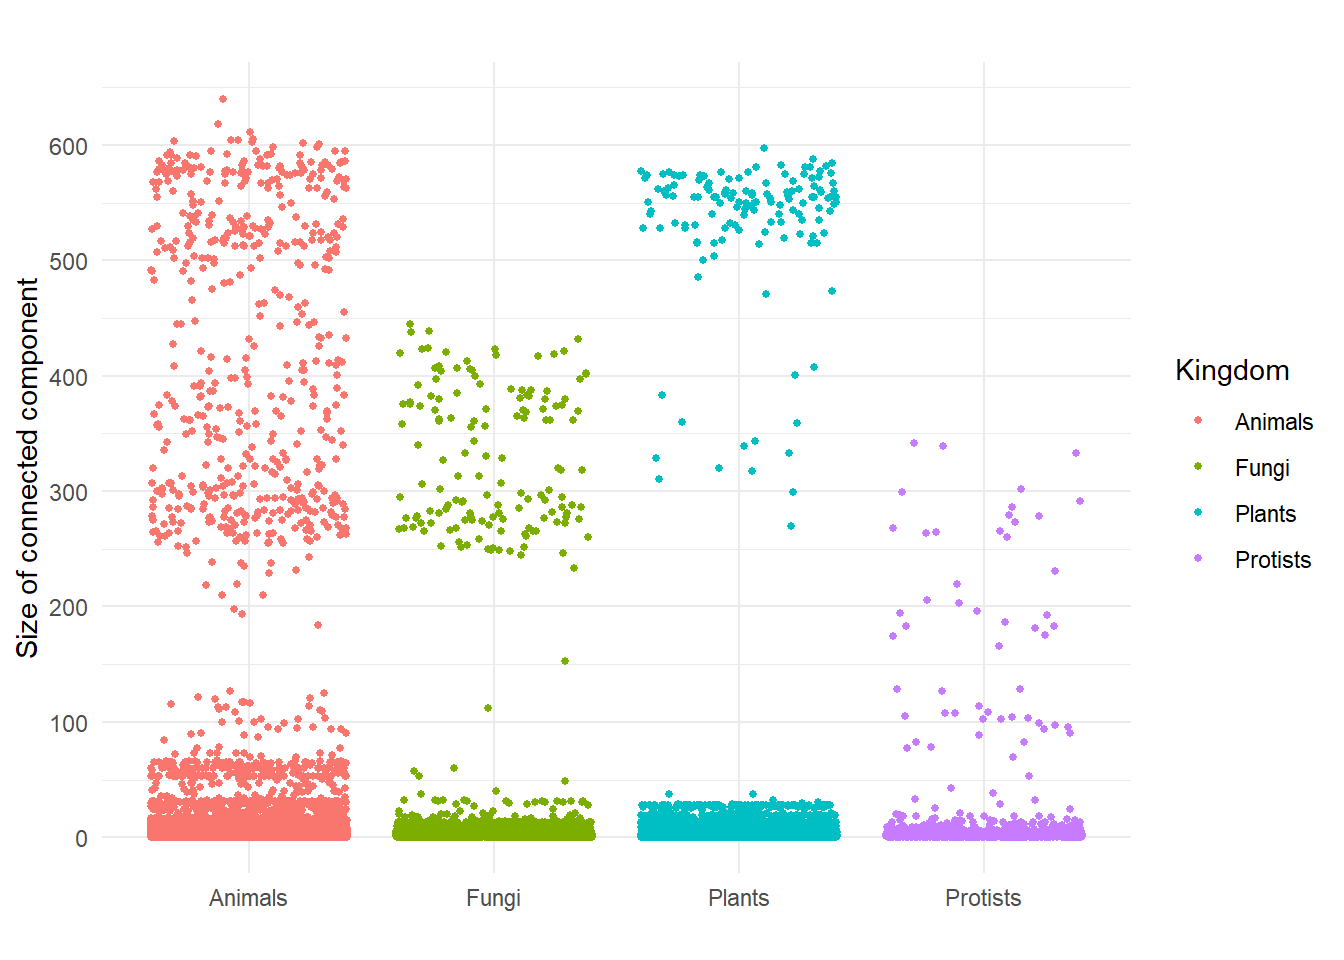
\includegraphics[width=1\textwidth,height=\textheight]{metabolic_graphs_files/figure-pdf/unnamed-chunk-20-1.pdf}

\begin{Shaded}
\begin{Highlighting}[]
\NormalTok{weak\_componets\_size\_max }\OtherTok{=}\NormalTok{ weak\_componets\_size }\SpecialCharTok{\%\textgreater{}\%}
  \FunctionTok{group\_by}\NormalTok{(Organism) }\SpecialCharTok{\%\textgreater{}\%}
  \FunctionTok{summarise}\NormalTok{(}\AttributeTok{csize =} \FunctionTok{max}\NormalTok{(csize),}\AttributeTok{Kingdom=}\FunctionTok{first}\NormalTok{(Kingdom))}
\CommentTok{\# Crear el gráfico de violín con puntos jitter}
\NormalTok{g }\OtherTok{\textless{}{-}} \FunctionTok{ggplot}\NormalTok{(weak\_componets\_size\_max, }\FunctionTok{aes}\NormalTok{(}\AttributeTok{x =}\NormalTok{ Kingdom, }\AttributeTok{y =}\NormalTok{ csize)) }\SpecialCharTok{+}
  \FunctionTok{geom\_violin}\NormalTok{(}\FunctionTok{aes}\NormalTok{(}\AttributeTok{fill =}\NormalTok{ Kingdom), }\AttributeTok{trim =} \ConstantTok{FALSE}\NormalTok{, }\AttributeTok{alpha =} \FloatTok{0.5}\NormalTok{) }\SpecialCharTok{+}  \CommentTok{\# Gráfico de violín con relleno por \textquotesingle{}Kingdom\textquotesingle{} y sin recortar}
  \FunctionTok{geom\_jitter}\NormalTok{(}\FunctionTok{aes}\NormalTok{(}\AttributeTok{color =}\NormalTok{ Kingdom), }\AttributeTok{size =} \DecValTok{1}\NormalTok{, }\AttributeTok{width =} \FloatTok{0.2}\NormalTok{) }\SpecialCharTok{+}  \CommentTok{\# Puntos con jitter para evitar solapamientos}
  \FunctionTok{xlab}\NormalTok{(}\StringTok{""}\NormalTok{) }\SpecialCharTok{+}  \CommentTok{\# Eliminar el título del eje X}
  \FunctionTok{ylab}\NormalTok{(}\StringTok{"Size of  largest weakly connected component"}\NormalTok{) }\SpecialCharTok{+}  \CommentTok{\# Etiqueta del eje Y}
  \FunctionTok{scale\_y\_continuous}\NormalTok{(}\AttributeTok{breaks =} \FunctionTok{seq}\NormalTok{(}\DecValTok{0}\NormalTok{, }\DecValTok{640}\NormalTok{, }\AttributeTok{by =} \DecValTok{100}\NormalTok{)) }\SpecialCharTok{+}  \CommentTok{\# Escala del eje Y con saltos de 100}
  \FunctionTok{theme\_minimal}\NormalTok{() }\SpecialCharTok{+}  \CommentTok{\# Tema minimalista con fondo blanco}
  \FunctionTok{ggtitle}\NormalTok{(}\StringTok{"Size of the largest weakly connected component by Kingdom }\SpecialCharTok{\textbackslash{}n}\StringTok{ (Violin Plot with Jittered Points)"}\NormalTok{)  }\CommentTok{\# Título del gráfico}

\CommentTok{\# Mostrar el gráfico}
\NormalTok{g}
\end{Highlighting}
\end{Shaded}

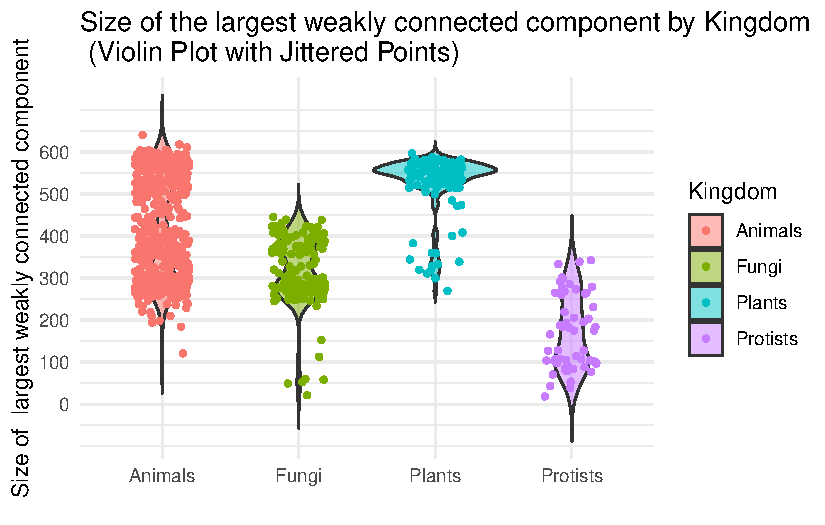
\includegraphics[width=1\textwidth,height=\textheight]{metabolic_graphs_files/figure-pdf/unnamed-chunk-21-1.pdf}

\bookmarksetup{startatroot}

\chapter{m-DAGs similarities and
Metadata}\label{m-dags-similarities-and-metadata}

\begin{Shaded}
\begin{Highlighting}[]
\FunctionTok{load}\NormalTok{(}\AttributeTok{file=}\StringTok{\textquotesingle{}metadag\_work\_space.RData\textquotesingle{}}\NormalTok{)}
\end{Highlighting}
\end{Shaded}

First, we will load the metadata and adjust them to match the structure
of the similarities. This will facilitate the creation of graphs and
statistics.

Keep in mind the path of the experiment:

\begin{Shaded}
\begin{Highlighting}[]
\NormalTok{experiment}\OtherTok{=}
  \StringTok{"0a845f74{-}826e{-}3b46{-}aed9{-}e7ecf74db262/"}
\NormalTok{path\_exp}\OtherTok{=}\FunctionTok{paste0}\NormalTok{(}\StringTok{"data/"}\NormalTok{,experiment)}
\end{Highlighting}
\end{Shaded}

\section{MSA \& Munkres similarities}\label{msa-munkres-similarities}

In this section, we will present the similarities between m-DAGs
considering the two similarity meausures described in the paper. Namely,
the MSA and Munkres similarities.

The experimental data set consists of 1132 Eukaryotes from the animal,
plant, fungus, and protists kingdoms.

\begin{longtable}[]{@{}lr@{}}
\toprule\noalign{}
Kingdom & Abs. Freq. \\
\midrule\noalign{}
\endhead
\bottomrule\noalign{}
\endlastfoot
Animals & 535 \\
Fungi & 154 \\
Plants & 139 \\
Protists & 56 \\
\end{longtable}

The similarity values are provided in the following files:

\begin{Shaded}
\begin{Highlighting}[]
\NormalTok{list\_Sim}\OtherTok{=}\FunctionTok{dir}\NormalTok{(path\_exp,}\AttributeTok{pattern=}\StringTok{"\^{}Similarities"}\NormalTok{)}
\NormalTok{list\_Sim}
\end{Highlighting}
\end{Shaded}

\begin{verbatim}
[1] "Similarities_MBB_MSAMethod.csv"      "Similarities_MBB_MunkresMethod.csv" 
[3] "Similarities_mDAG_MSAMethod.csv"     "Similarities_mDAG_MunkresMethod.csv"
\end{verbatim}

Load the m-DAGs similarities

\begin{Shaded}
\begin{Highlighting}[]
\NormalTok{n}\OtherTok{=}\DecValTok{884}\CommentTok{\# no synthetic mDGAs}
\NormalTok{Sim\_MSA\_mDAG}\OtherTok{=}\FunctionTok{read\_csv}\NormalTok{(}\FunctionTok{paste0}\NormalTok{(path\_exp,}
                             \StringTok{"Similarities\_mDAG\_MSAMethod.csv"}\NormalTok{))}
\NormalTok{Sim\_MSA\_mDAG}\OtherTok{=}\FunctionTok{as.matrix}\NormalTok{(Sim\_MSA\_mDAG[,}\SpecialCharTok{{-}}\DecValTok{1}\NormalTok{])}
\FunctionTok{rownames}\NormalTok{(Sim\_MSA\_mDAG)}\OtherTok{=}\FunctionTok{colnames}\NormalTok{(Sim\_MSA\_mDAG)}
\NormalTok{Sim\_MSA\_mDAG}\OtherTok{=}\NormalTok{Sim\_MSA\_mDAG[meta\_taxo}\SpecialCharTok{$}\NormalTok{mDAG\_Id[}\DecValTok{1}\SpecialCharTok{:}\NormalTok{n],}
\NormalTok{                          meta\_taxo}\SpecialCharTok{$}\NormalTok{mDAG\_Id[}\DecValTok{1}\SpecialCharTok{:}\NormalTok{n]]}
\end{Highlighting}
\end{Shaded}

\begin{Shaded}
\begin{Highlighting}[]
\NormalTok{Sim\_Mun\_mDAG}\OtherTok{=}\FunctionTok{read\_csv}\NormalTok{(}\FunctionTok{paste0}\NormalTok{(path\_exp,}\StringTok{"Similarities\_mDAG\_MunkresMethod.csv"}\NormalTok{))}
\NormalTok{Sim\_Mun\_mDAG}\OtherTok{=}\FunctionTok{as.matrix}\NormalTok{(Sim\_Mun\_mDAG[,}\SpecialCharTok{{-}}\DecValTok{1}\NormalTok{])}
\FunctionTok{rownames}\NormalTok{(Sim\_Mun\_mDAG)}\OtherTok{=}\FunctionTok{colnames}\NormalTok{(Sim\_Mun\_mDAG)}
\NormalTok{Sim\_Mun\_mDAG}\OtherTok{=}\NormalTok{Sim\_Mun\_mDAG[meta\_taxo}\SpecialCharTok{$}\NormalTok{mDAG\_Id[}\DecValTok{1}\SpecialCharTok{:}\NormalTok{n],meta\_taxo}\SpecialCharTok{$}\NormalTok{mDAG\_Id[}\DecValTok{1}\SpecialCharTok{:}\NormalTok{n]]}
\end{Highlighting}
\end{Shaded}

\section{Heatmaps}\label{heatmaps}

Here, we provide examples of heatmaps to visualize the similarities
betweem m-DAGs. We again consider colors to represent the different
Kingdoms.

\begin{Shaded}
\begin{Highlighting}[]
\NormalTok{dff}\OtherTok{\textless{}{-}}\NormalTok{meta\_taxo[}\DecValTok{1}\SpecialCharTok{:}\DecValTok{884}\NormalTok{,] }\SpecialCharTok{\%\textgreater{}\%} \FunctionTok{select}\NormalTok{(Kingdom)  }\SpecialCharTok{\%\textgreater{}\%} \FunctionTok{as.data.frame}\NormalTok{()}
\NormalTok{colorsK }\OtherTok{\textless{}{-}} \FunctionTok{list}\NormalTok{(}\AttributeTok{Kingdom=} \FunctionTok{c}\NormalTok{(}\StringTok{"Animals"}\OtherTok{=}\StringTok{"red"}\NormalTok{,}
                           \StringTok{"Plants"}\OtherTok{=}\StringTok{"green"}\NormalTok{,}
                           \StringTok{"Fungi"}\OtherTok{=}\StringTok{"yellow"}\NormalTok{,}
                           \StringTok{"Protists"}\OtherTok{=}\StringTok{"black"}\NormalTok{))}
\NormalTok{annotationK }\OtherTok{\textless{}{-}} \FunctionTok{HeatmapAnnotation}\NormalTok{(}\AttributeTok{df=}\NormalTok{dff, }\AttributeTok{col =}\NormalTok{ colorsK,}\AttributeTok{show\_legend =} \ConstantTok{TRUE}\NormalTok{)}

\NormalTok{MSA\_heat\_1 }\OtherTok{\textless{}{-}} \FunctionTok{Heatmap}\NormalTok{(}\AttributeTok{matrix =}\NormalTok{ Sim\_MSA\_mDAG, }
                      \AttributeTok{column\_title=}
                        \StringTok{"m{-}DAGs MSA{-}similarity Eukaryotes by Kingdoms"}\NormalTok{,}
                      \AttributeTok{heatmap\_legend\_param=}\FunctionTok{list}\NormalTok{(}
                        \AttributeTok{title=}\StringTok{"Similarity"}\NormalTok{,}
                        \AttributeTok{at =} \FunctionTok{seq}\NormalTok{(}\DecValTok{0}\NormalTok{,}\DecValTok{1}\NormalTok{,}\AttributeTok{by=}\FloatTok{0.1}\NormalTok{)),}
                      \AttributeTok{col=}\FunctionTok{rev}\NormalTok{(}\FunctionTok{viridis}\NormalTok{(}\DecValTok{256}\NormalTok{)),}
                      \AttributeTok{cluster\_rows =} \ConstantTok{FALSE}\NormalTok{,}
                      \AttributeTok{cluster\_columns =} \ConstantTok{FALSE}\NormalTok{,}
                      \AttributeTok{top\_annotation =}\NormalTok{ annotationK,}
                      \AttributeTok{show\_column\_names =} \ConstantTok{FALSE}\NormalTok{, }
                      \AttributeTok{show\_row\_names =} \ConstantTok{FALSE}\NormalTok{,}
                      \AttributeTok{left\_annotation =}
                        \FunctionTok{rowAnnotation}\NormalTok{(}\AttributeTok{df =}\NormalTok{ dff,}
                                      \AttributeTok{col =}\NormalTok{ colorsK,}
                                    \AttributeTok{show\_annotation\_name=}\ConstantTok{FALSE}\NormalTok{,}
                                    \AttributeTok{show\_legend=}\ConstantTok{FALSE}
\NormalTok{                                      ))}


\NormalTok{Mun\_heat\_1 }\OtherTok{\textless{}{-}} \FunctionTok{Heatmap}\NormalTok{(}\AttributeTok{matrix =}\NormalTok{ Sim\_Mun\_mDAG, }
             \AttributeTok{column\_title=}\StringTok{"m{-}DAGs Munkres{-}similarity  Eukaryotes by Kingdoms"}\NormalTok{,}
            \AttributeTok{name =} \StringTok{"Munkres Similarity"}\NormalTok{,}
            \AttributeTok{heatmap\_legend\_param=}\FunctionTok{list}\NormalTok{(}
                        \AttributeTok{title=}\StringTok{"Similarity"}\NormalTok{,}
                        \AttributeTok{at =} \FunctionTok{seq}\NormalTok{(}\DecValTok{0}\NormalTok{,}\DecValTok{1}\NormalTok{,}\AttributeTok{by=}\FloatTok{0.1}\NormalTok{)),}
                      \AttributeTok{col=}\FunctionTok{rev}\NormalTok{(}\FunctionTok{viridis}\NormalTok{(}\DecValTok{256}\NormalTok{)),}
                      \AttributeTok{cluster\_rows =} \ConstantTok{FALSE}\NormalTok{,}
                      \AttributeTok{cluster\_columns =} \ConstantTok{FALSE}\NormalTok{,}
                      \AttributeTok{top\_annotation =}\NormalTok{ annotationK,}
                      \AttributeTok{show\_column\_names =} \ConstantTok{FALSE}\NormalTok{, }
                      \AttributeTok{show\_row\_names =} \ConstantTok{FALSE}\NormalTok{,}
                      \AttributeTok{left\_annotation =}
                        \FunctionTok{rowAnnotation}\NormalTok{(}\AttributeTok{df =}\NormalTok{ dff,}
                                      \AttributeTok{col =}\NormalTok{ colorsK,}
                                    \AttributeTok{show\_annotation\_name=}\ConstantTok{FALSE}\NormalTok{,}
                                    \AttributeTok{show\_legend=}\ConstantTok{FALSE}\NormalTok{                                                                        ))}
\end{Highlighting}
\end{Shaded}

\begin{Shaded}
\begin{Highlighting}[]
\DocumentationTok{\#\#  Animals by phylum}

\NormalTok{meta\_animals  }\OtherTok{=}\NormalTok{ meta\_taxo }\SpecialCharTok{\%\textgreater{}\%} \FunctionTok{filter}\NormalTok{(Kingdom}\SpecialCharTok{==}\StringTok{"Animals"}\NormalTok{)}
\NormalTok{namesP}\OtherTok{=}\FunctionTok{names}\NormalTok{(}\FunctionTok{rev}\NormalTok{(}\FunctionTok{sort}\NormalTok{(}\FunctionTok{table}\NormalTok{(meta\_animals}\SpecialCharTok{$}\NormalTok{Phylum))))}
\NormalTok{namesP}
\end{Highlighting}
\end{Shaded}

\begin{verbatim}
 [1] "Vertebrates"      "Arthropods"       "Mollusks"         "Cnidarians"      
 [5] "Nematodes"        "Flatworms"        "Echinoderms"      "Tunicates"       
 [9] "Cephalochordates" "Poriferans"       "Placozoans"       "Hemichordates"   
[13] "Brachiopodas"     "Annelids"        
\end{verbatim}

\begin{Shaded}
\begin{Highlighting}[]
\NormalTok{dff}\OtherTok{=}\FunctionTok{data.frame}\NormalTok{(}\AttributeTok{Phylum=}\NormalTok{meta\_animals}\SpecialCharTok{$}\NormalTok{Phylum)}
\NormalTok{Phylum}\OtherTok{=}\FunctionTok{ordered}\NormalTok{(meta\_animals}\SpecialCharTok{$}\NormalTok{Phylum,}\AttributeTok{levels=}\NormalTok{namesP)}
\NormalTok{numbersP}\OtherTok{=}\FunctionTok{paste}\NormalTok{(}\FunctionTok{c}\NormalTok{(}\FunctionTok{paste0}\NormalTok{(}\DecValTok{0}\NormalTok{,}\DecValTok{1}\SpecialCharTok{:}\DecValTok{9}\NormalTok{),}\DecValTok{10}\SpecialCharTok{:}\DecValTok{14}\NormalTok{),namesP,}\AttributeTok{sep=}\StringTok{"{-}"}\NormalTok{)}
\FunctionTok{levels}\NormalTok{(Phylum)}\OtherTok{=}\NormalTok{numbersP}
\NormalTok{dff}\SpecialCharTok{$}\NormalTok{Phylum}\OtherTok{=}\NormalTok{Phylum}
\NormalTok{col}\OtherTok{=}\FunctionTok{rainbow}\NormalTok{(}\FunctionTok{length}\NormalTok{(namesP))}

\NormalTok{colorsP}\OtherTok{=}\FunctionTok{list}\NormalTok{(}\AttributeTok{Phylum=}\NormalTok{col)}
\FunctionTok{names}\NormalTok{(colorsP}\SpecialCharTok{$}\NormalTok{Phylum)}\OtherTok{=}\NormalTok{numbersP}

\NormalTok{annot }\OtherTok{\textless{}{-}} \FunctionTok{HeatmapAnnotation}\NormalTok{(}\AttributeTok{df =}\NormalTok{ dff, }
                               \AttributeTok{col =}\NormalTok{ colorsP,}
                               \AttributeTok{annotation\_name\_side =} \StringTok{"left"}\NormalTok{,}
                               \AttributeTok{show\_annotation\_name=}\ConstantTok{TRUE}\NormalTok{ )}

\NormalTok{MSA\_heat\_2 }\OtherTok{\textless{}{-}}  \FunctionTok{Heatmap}\NormalTok{(}
  \AttributeTok{matrix =}\NormalTok{ Sim\_MSA\_mDAG[meta\_animals}\SpecialCharTok{$}\NormalTok{mDAG\_Id,}
\NormalTok{                        meta\_animals}\SpecialCharTok{$}\NormalTok{mDAG\_Id],}
  \AttributeTok{name =} \StringTok{"MSA similarity"}\NormalTok{,}
  \AttributeTok{column\_title =} \StringTok{"m{-}DAGs MSA{-}similarity  Animals by Phyla"}\NormalTok{,}
  \AttributeTok{col =} \FunctionTok{rev}\NormalTok{(}\FunctionTok{viridis}\NormalTok{(}\DecValTok{256}\NormalTok{)),}
  \AttributeTok{cluster\_rows =} \ConstantTok{FALSE}\NormalTok{,}
  \AttributeTok{show\_heatmap\_legend =} \ConstantTok{FALSE}\NormalTok{,}
  \AttributeTok{cluster\_columns =} \ConstantTok{FALSE}\NormalTok{,}
  \AttributeTok{top\_annotation =}\NormalTok{ annot,}
  \AttributeTok{show\_column\_names =} \ConstantTok{FALSE}\NormalTok{,}
  \AttributeTok{show\_row\_names =} \ConstantTok{FALSE}\NormalTok{,}
  \AttributeTok{left\_annotation =}
    \FunctionTok{rowAnnotation}\NormalTok{(}
      \AttributeTok{df =}\NormalTok{ dff,}
      \AttributeTok{col =}\NormalTok{ colorsP,}
      \AttributeTok{show\_annotation\_name =} \ConstantTok{FALSE}
\NormalTok{    )}
\NormalTok{)}




\NormalTok{Mun\_heat\_2 }\OtherTok{\textless{}{-}} \FunctionTok{Heatmap}\NormalTok{(}
  \AttributeTok{matrix =}\NormalTok{ Sim\_Mun\_mDAG[meta\_animals}\SpecialCharTok{$}\NormalTok{mDAG\_Id,}
\NormalTok{                        meta\_animals}\SpecialCharTok{$}\NormalTok{mDAG\_Id],}
  \AttributeTok{column\_title =} \StringTok{"m{-}DAGs Munkres{-}similarity  Animals by Phyla"}\NormalTok{,}
 \AttributeTok{col =} \FunctionTok{rev}\NormalTok{(}\FunctionTok{viridis}\NormalTok{(}\DecValTok{256}\NormalTok{)),}
  \AttributeTok{cluster\_rows =} \ConstantTok{FALSE}\NormalTok{,}
  \AttributeTok{show\_heatmap\_legend =} \ConstantTok{FALSE}\NormalTok{,}
  \AttributeTok{cluster\_columns =} \ConstantTok{FALSE}\NormalTok{,}
  \AttributeTok{top\_annotation =}\NormalTok{ annot,}
  \AttributeTok{show\_column\_names =} \ConstantTok{FALSE}\NormalTok{,}
  \AttributeTok{show\_row\_names =} \ConstantTok{FALSE}\NormalTok{,}
  \AttributeTok{left\_annotation =}
    \FunctionTok{rowAnnotation}\NormalTok{(}
      \AttributeTok{df =}\NormalTok{ dff,}
      \AttributeTok{col =}\NormalTok{ colorsP,}
      \AttributeTok{show\_annotation\_name =} \ConstantTok{FALSE}
\NormalTok{    )}
\NormalTok{)}
\end{Highlighting}
\end{Shaded}

\begin{Shaded}
\begin{Highlighting}[]
\FunctionTok{draw}\NormalTok{(MSA\_heat\_1,}\AttributeTok{merge\_legend=}\ConstantTok{TRUE}\NormalTok{)}
\end{Highlighting}
\end{Shaded}

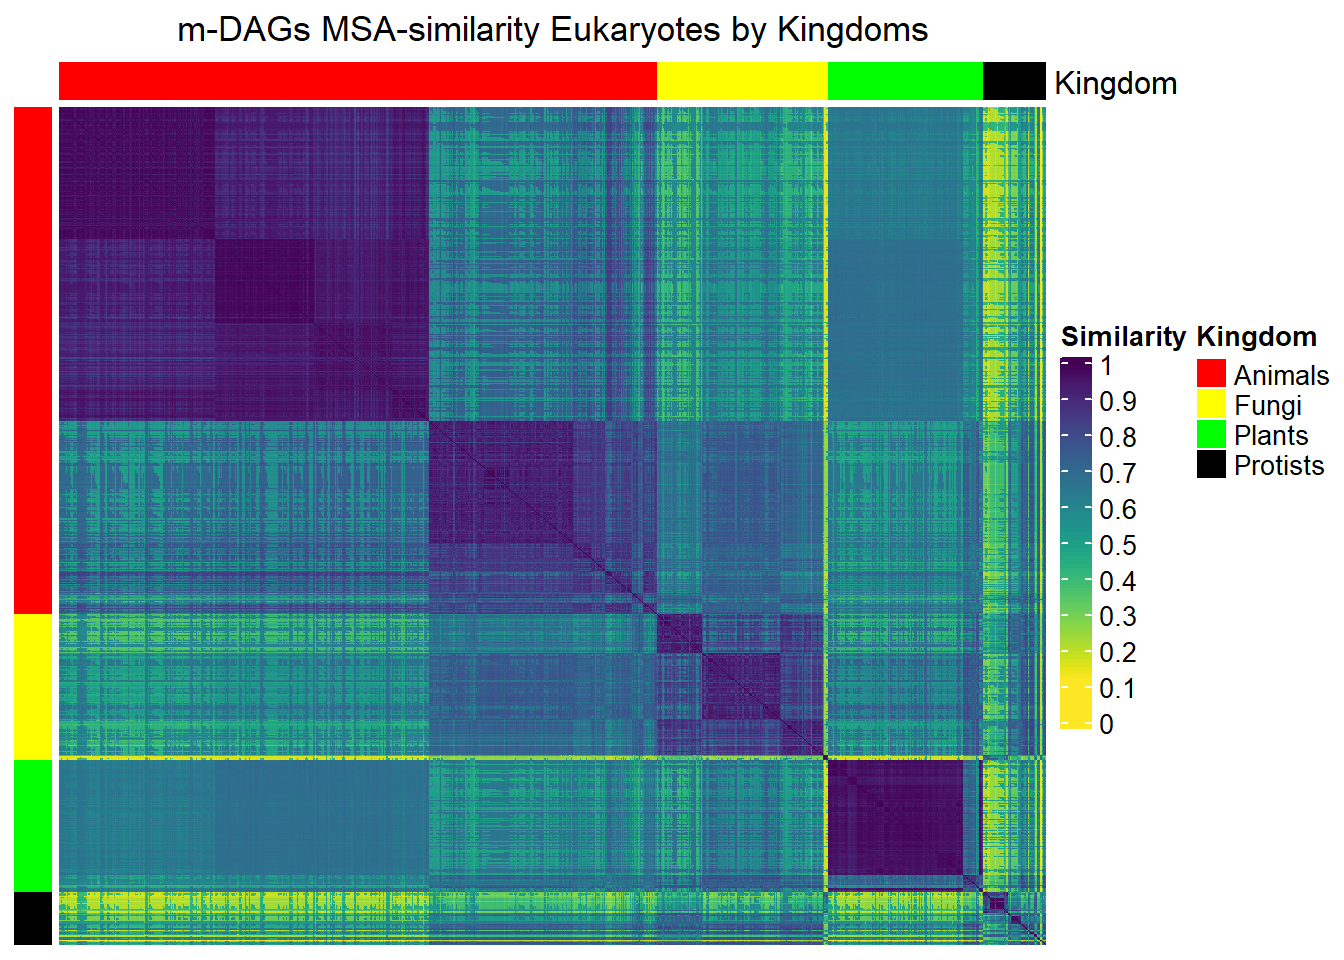
\includegraphics[width=1\textwidth,height=\textheight]{m_DAGs_similarity_files/figure-pdf/heatmaps-1.pdf}

\begin{Shaded}
\begin{Highlighting}[]
\FunctionTok{draw}\NormalTok{(MSA\_heat\_2,}\AttributeTok{merge\_legend=}\ConstantTok{TRUE}\NormalTok{)}
\end{Highlighting}
\end{Shaded}

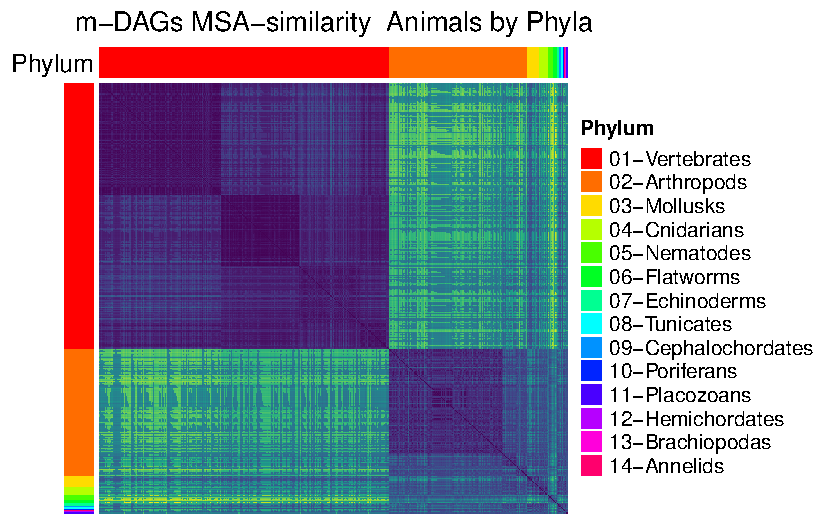
\includegraphics[width=1\textwidth,height=\textheight]{m_DAGs_similarity_files/figure-pdf/heatmaps-2.pdf}

\begin{Shaded}
\begin{Highlighting}[]
\FunctionTok{draw}\NormalTok{(Mun\_heat\_1,}\AttributeTok{merge\_legend=}\ConstantTok{TRUE}\NormalTok{)}
\end{Highlighting}
\end{Shaded}

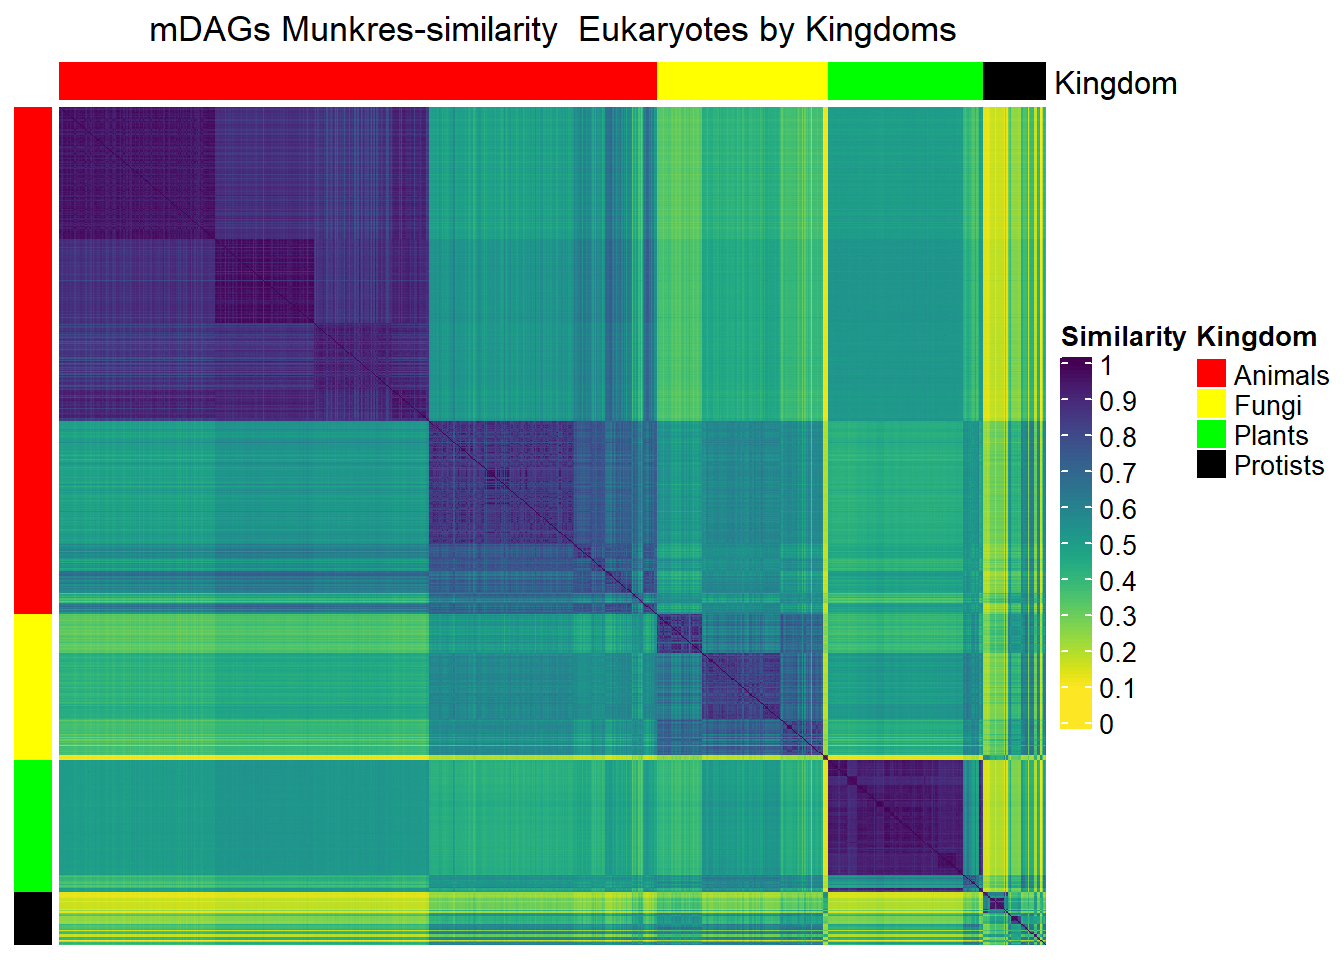
\includegraphics[width=1\textwidth,height=\textheight]{m_DAGs_similarity_files/figure-pdf/heatmaps-3.pdf}

\begin{Shaded}
\begin{Highlighting}[]
\FunctionTok{draw}\NormalTok{(Mun\_heat\_2,}\AttributeTok{merge\_legend=}\ConstantTok{TRUE}\NormalTok{)}
\end{Highlighting}
\end{Shaded}

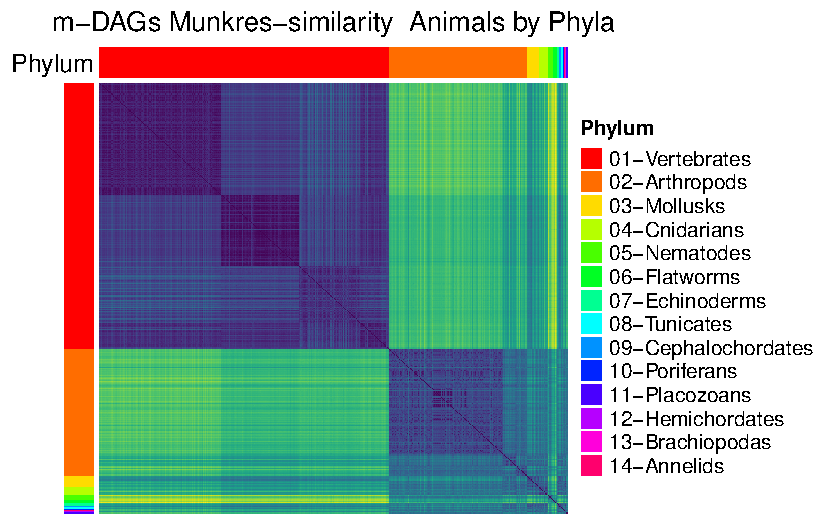
\includegraphics[width=1\textwidth,height=\textheight]{m_DAGs_similarity_files/figure-pdf/heatmaps-4.pdf}

\section{MDS (Multidimensional Scaling) MSA \& Munkres
similarities}\label{mds-multidimensional-scaling-msa-munkres-similarities}

Multi-dimensional Scaling (MDS) is a classic multivariate data analysis
technique that allows for obtaining a low-dimensional representation of
the observed similarities. First, we transform each similarity measure
into a distance measure as follows: let \(s_{ij}\) be a similarity
measure between a pair \(i,j\), we define its distance measure as
\(d_{ij}=\sqrt{1-s_{ij}^2}\).

The following is the MDS for the MSA distance:

\begin{Shaded}
\begin{Highlighting}[]
\DocumentationTok{\#\# Metric multidimensional scaling (mMDS)}
\NormalTok{mds7 }\OtherTok{\textless{}{-}} \FunctionTok{cmdscale}\NormalTok{(}\FunctionTok{sqrt}\NormalTok{(}\DecValTok{1}\SpecialCharTok{{-}}\NormalTok{Sim\_MSA\_mDAG}\SpecialCharTok{\^{}}\DecValTok{2}\NormalTok{),}\AttributeTok{k=}\DecValTok{7}\NormalTok{,}\AttributeTok{eig=}\ConstantTok{TRUE}\NormalTok{)}
\NormalTok{mds7}\SpecialCharTok{$}\NormalTok{GOF}
\end{Highlighting}
\end{Shaded}

\begin{verbatim}
[1] 0.4449519 0.5570199
\end{verbatim}

\begin{Shaded}
\begin{Highlighting}[]
\NormalTok{mds }\OtherTok{\textless{}{-}}\NormalTok{ mds7}\SpecialCharTok{$}\NormalTok{points }\SpecialCharTok{\%\textgreater{}\%}  \FunctionTok{as\_tibble}\NormalTok{()}
\FunctionTok{colnames}\NormalTok{(mds) }\OtherTok{\textless{}{-}}\FunctionTok{paste0}\NormalTok{(}\StringTok{"Dim."}\NormalTok{,}\DecValTok{1}\SpecialCharTok{:}\FunctionTok{dim}\NormalTok{(mds7}\SpecialCharTok{$}\NormalTok{points)[}\DecValTok{2}\NormalTok{])}


\NormalTok{cooordinates}\OtherTok{=}\FunctionTok{as\_tibble}\NormalTok{(mds7}\SpecialCharTok{$}\NormalTok{points)}
\FunctionTok{colnames}\NormalTok{(cooordinates)}\OtherTok{=}\FunctionTok{paste}\NormalTok{(}\StringTok{"Component"}\NormalTok{,}\DecValTok{1}\SpecialCharTok{:}\DecValTok{7}\NormalTok{)}
\FunctionTok{ggpairs}\NormalTok{(cooordinates,}\AttributeTok{columns=}\DecValTok{1}\SpecialCharTok{:}\DecValTok{4}\NormalTok{,}
        \FunctionTok{aes}\NormalTok{(}\AttributeTok{color=}\NormalTok{meta\_taxo}\SpecialCharTok{$}\NormalTok{Kingdom[}\DecValTok{1}\SpecialCharTok{:}\DecValTok{884}\NormalTok{],}
            \AttributeTok{title=}\StringTok{"MDS 4 dimensions projection"}\NormalTok{,}\AttributeTok{legend=}\DecValTok{1}\NormalTok{),}
        \AttributeTok{lower=}\FunctionTok{list}\NormalTok{(}\AttributeTok{continuous=}\StringTok{"points"}\NormalTok{)) }\SpecialCharTok{+} 
  \FunctionTok{scale\_fill\_manual}\NormalTok{(}\AttributeTok{values =}\NormalTok{ colorsK}\SpecialCharTok{$}\NormalTok{Kingdom) }\SpecialCharTok{+} 
  \FunctionTok{theme}\NormalTok{(}\AttributeTok{legend.position =} \StringTok{"left"}\NormalTok{)}
\end{Highlighting}
\end{Shaded}

\begin{center}
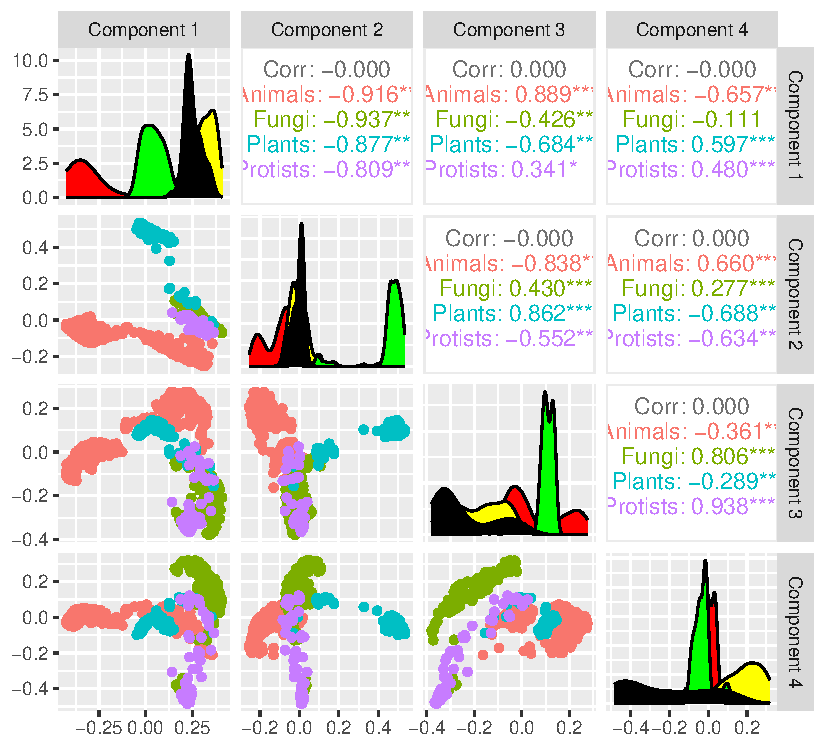
\includegraphics[width=1\textwidth,height=\textheight]{m_DAGs_similarity_files/figure-pdf/unnamed-chunk-11-1.pdf}
\end{center}

The following is the MDS for the Munkres distance:

\begin{Shaded}
\begin{Highlighting}[]
\DocumentationTok{\#\# Metric multidimensional scaling}
\NormalTok{mds7 }\OtherTok{\textless{}{-}} \FunctionTok{cmdscale}\NormalTok{(}\FunctionTok{sqrt}\NormalTok{(}\DecValTok{1}\SpecialCharTok{{-}}\NormalTok{Sim\_Mun\_mDAG}\SpecialCharTok{\^{}}\DecValTok{2}\NormalTok{),}\AttributeTok{k=}\DecValTok{7}\NormalTok{,}\AttributeTok{eig=}\ConstantTok{TRUE}\NormalTok{)}
\NormalTok{mds7}\SpecialCharTok{$}\NormalTok{GOF}
\end{Highlighting}
\end{Shaded}

\begin{verbatim}
[1] 0.5605691 0.5800736
\end{verbatim}

\begin{Shaded}
\begin{Highlighting}[]
\NormalTok{mds }\OtherTok{\textless{}{-}}\NormalTok{ mds7}\SpecialCharTok{$}\NormalTok{points }\SpecialCharTok{\%\textgreater{}\%}  \FunctionTok{as\_tibble}\NormalTok{()}
\FunctionTok{colnames}\NormalTok{(mds) }\OtherTok{\textless{}{-}}\FunctionTok{paste0}\NormalTok{(}\StringTok{"Dim."}\NormalTok{,}\DecValTok{1}\SpecialCharTok{:}\FunctionTok{dim}\NormalTok{(mds7}\SpecialCharTok{$}\NormalTok{points)[}\DecValTok{2}\NormalTok{])}

\NormalTok{cooordinates}\OtherTok{=}\FunctionTok{as\_tibble}\NormalTok{(mds7}\SpecialCharTok{$}\NormalTok{points)}
\FunctionTok{colnames}\NormalTok{(cooordinates)}\OtherTok{=}\FunctionTok{paste}\NormalTok{(}\StringTok{"Component"}\NormalTok{,}\DecValTok{1}\SpecialCharTok{:}\DecValTok{7}\NormalTok{)}
\FunctionTok{ggpairs}\NormalTok{(cooordinates,}\AttributeTok{columns=}\DecValTok{1}\SpecialCharTok{:}\DecValTok{4}\NormalTok{,}
        \FunctionTok{aes}\NormalTok{(}\AttributeTok{color=}\NormalTok{meta\_taxo}\SpecialCharTok{$}\NormalTok{Kingdom[}\DecValTok{1}\SpecialCharTok{:}\DecValTok{884}\NormalTok{],}
            \AttributeTok{title=}\StringTok{"MDS 4 dimensions projection"}\NormalTok{,}\AttributeTok{legend=}\DecValTok{1}\NormalTok{),}
        \AttributeTok{lower=}\FunctionTok{list}\NormalTok{(}\AttributeTok{continuous=}\StringTok{"points"}\NormalTok{)) }\SpecialCharTok{+} 
  \FunctionTok{scale\_fill\_manual}\NormalTok{(}\AttributeTok{values =}\NormalTok{ colorsK}\SpecialCharTok{$}\NormalTok{Kingdom) }\SpecialCharTok{+} 
  \FunctionTok{theme}\NormalTok{(}\AttributeTok{legend.position =} \StringTok{"left"}\NormalTok{)}
\end{Highlighting}
\end{Shaded}

\begin{center}
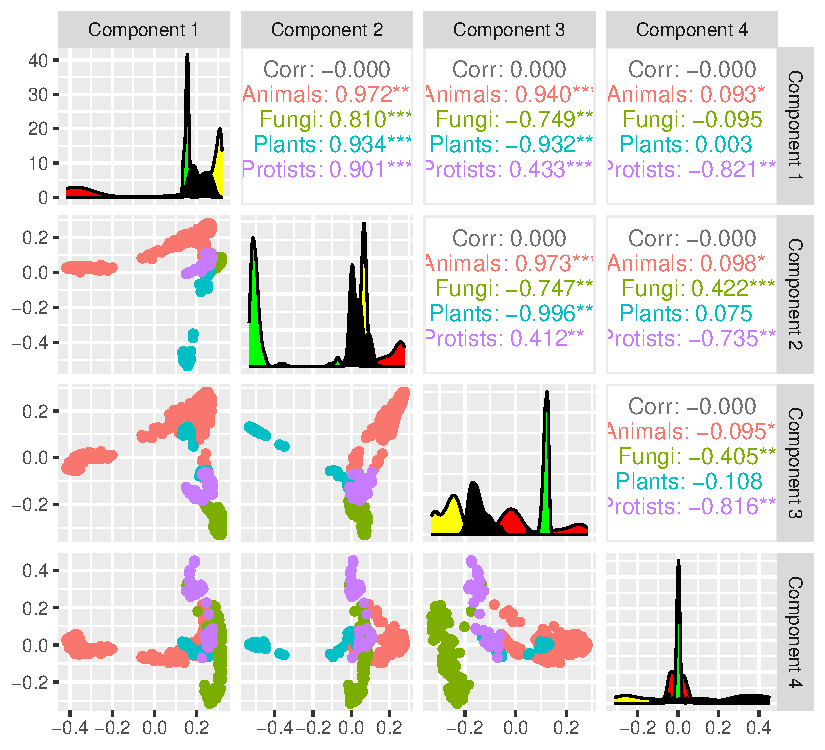
\includegraphics[width=1\textwidth,height=\textheight]{m_DAGs_similarity_files/figure-pdf/unnamed-chunk-12-1.pdf}
\end{center}

\section{Hierarchical clustering MSA
similarity}\label{hierarchical-clustering-msa-similarity}

Through hierarchical clustering using the Ward method, we have derived a
partition of the m-DAGs into 4, 5, and 6 clusters, respectively. The
corresponding information has been organized into a table, as follows:

\begin{Shaded}
\begin{Highlighting}[]
\NormalTok{D}\OtherTok{=}\FunctionTok{as.dist}\NormalTok{(}\FunctionTok{sqrt}\NormalTok{(}\DecValTok{1}\SpecialCharTok{{-}}\NormalTok{Sim\_MSA\_mDAG}\SpecialCharTok{\^{}}\DecValTok{2}\NormalTok{))}
\NormalTok{hc\_MSA}\OtherTok{=}\FunctionTok{hclust}\NormalTok{(}\FunctionTok{as.dist}\NormalTok{(D),}\AttributeTok{method =}\StringTok{"ward.D"}\NormalTok{)}
\NormalTok{clust4\_MSA}\OtherTok{=}\FunctionTok{cutree}\NormalTok{(hc\_MSA,}\DecValTok{4}\NormalTok{)}
\FunctionTok{table}\NormalTok{(clust4\_MSA,meta\_taxo}\SpecialCharTok{$}\NormalTok{Kingdom[}\DecValTok{1}\SpecialCharTok{:}\DecValTok{884}\NormalTok{])}
\end{Highlighting}
\end{Shaded}

\begin{verbatim}
          
clust4_MSA Animals Fungi Plants Protists
         1     331     0      0        0
         2     197     0      0        0
         3       7   154     14       56
         4       0     0    125        0
\end{verbatim}

\begin{Shaded}
\begin{Highlighting}[]
\NormalTok{clust5\_MSA}\OtherTok{=}\FunctionTok{cutree}\NormalTok{(hc\_MSA,}\DecValTok{5}\NormalTok{)}
\FunctionTok{table}\NormalTok{(clust5\_MSA,meta\_taxo}\SpecialCharTok{$}\NormalTok{Kingdom[}\DecValTok{1}\SpecialCharTok{:}\DecValTok{884}\NormalTok{])}
\end{Highlighting}
\end{Shaded}

\begin{verbatim}
          
clust5_MSA Animals Fungi Plants Protists
         1     129     0      0        0
         2     202     0      0        0
         3     197     0      0        0
         4       7   154     14       56
         5       0     0    125        0
\end{verbatim}

\begin{Shaded}
\begin{Highlighting}[]
\NormalTok{clust6\_MSA}\OtherTok{=}\FunctionTok{cutree}\NormalTok{(hc\_MSA,}\DecValTok{6}\NormalTok{)}
\FunctionTok{table}\NormalTok{(clust6\_MSA,meta\_taxo}\SpecialCharTok{$}\NormalTok{Kingdom[}\DecValTok{1}\SpecialCharTok{:}\DecValTok{884}\NormalTok{])}
\end{Highlighting}
\end{Shaded}

\begin{verbatim}
          
clust6_MSA Animals Fungi Plants Protists
         1     129     0      0        0
         2     202     0      0        0
         3     197     0      0        0
         4       7   149     14       34
         5       0     5      0       22
         6       0     0    125        0
\end{verbatim}

We can also create a table that correlates the clusters (in this case,
two clusters) with the Phylum classification:

\begin{Shaded}
\begin{Highlighting}[]
\NormalTok{aux}\OtherTok{=}\NormalTok{meta\_taxo[}\DecValTok{1}\SpecialCharTok{:}\DecValTok{884}\NormalTok{,] }\SpecialCharTok{\%\textgreater{}\%}
  \FunctionTok{select}\NormalTok{(Organism,Kingdom,Phylum,Class,Full\_Name)}
\NormalTok{aux}\SpecialCharTok{$}\NormalTok{clust4\_MSA}\OtherTok{=}\NormalTok{clust4\_MSA}
\NormalTok{aux\_Animals\_cluster\_1\_2 }\OtherTok{=}\NormalTok{ aux }\SpecialCharTok{\%\textgreater{}\%}
  \FunctionTok{filter}\NormalTok{(Kingdom}\SpecialCharTok{==}\StringTok{"Animals"}\NormalTok{,clust4\_MSA }\SpecialCharTok{\%in\%} \FunctionTok{c}\NormalTok{(}\DecValTok{1}\NormalTok{,}\DecValTok{2}\NormalTok{))}

\FunctionTok{table}\NormalTok{(aux\_Animals\_cluster\_1\_2}\SpecialCharTok{$}\NormalTok{Phylum,aux\_Animals\_cluster\_1\_2}\SpecialCharTok{$}\NormalTok{clust4\_MSA)}
\end{Highlighting}
\end{Shaded}

\begin{verbatim}
                  
                     1   2
  Annelids           0   1
  Arthropods         0 158
  Brachiopodas       0   1
  Cephalochordates   0   2
  Cnidarians         0  10
  Echinoderms        0   3
  Hemichordates      0   1
  Mollusks           0  14
  Nematodes          0   3
  Placozoans         0   1
  Poriferans         0   1
  Tunicates          0   2
  Vertebrates      331   0
\end{verbatim}

We can retrieve the information of the elements belonging to a specific
classification (Animals and Plants) that are part of a particular
cluster as follows:

\begin{Shaded}
\begin{Highlighting}[]
\NormalTok{aux\_7\_Animals\_cluster\_3}\OtherTok{=} \FunctionTok{filter}\NormalTok{(aux,}
\NormalTok{                                clust4\_MSA}\SpecialCharTok{==}\DecValTok{3}\NormalTok{,}
\NormalTok{                                Kingdom}\SpecialCharTok{==}\StringTok{"Animals"}\NormalTok{)}
\NormalTok{aux\_7\_Animals\_cluster\_3}
\end{Highlighting}
\end{Shaded}

\begin{verbatim}
# A tibble: 7 x 6
  Organism Kingdom Phylum    Class     Full_Name                      clust4_MSA
  <chr>    <chr>   <chr>     <chr>     <chr>                               <int>
1 bmy      Animals Nematodes Nematodes Brugia malayi (filaria)                 3
2 loa      Animals Nematodes Nematodes Loa loa (eye worm)                      3
3 tsp      Animals Nematodes Nematodes Trichinella spiralis                    3
4 egl      Animals Flatworms Flatworms Echinococcus granulosus (hyda~          3
5 ovi      Animals Flatworms Flatworms Opisthorchis viverrini (South~          3
6 shx      Animals Flatworms Flatworms Schistosoma haematobium (urin~          3
7 smm      Animals Flatworms Flatworms Schistosoma mansoni                     3
\end{verbatim}

\begin{Shaded}
\begin{Highlighting}[]
\NormalTok{aux\_14\_Plants\_clust\_3}\OtherTok{=} \FunctionTok{filter}\NormalTok{(aux,clust4\_MSA}\SpecialCharTok{==}\DecValTok{3}\NormalTok{,}
\NormalTok{                             Kingdom}\SpecialCharTok{==}\StringTok{"Plants"}\NormalTok{)}
\NormalTok{aux\_14\_Plants\_clust\_3}
\end{Highlighting}
\end{Shaded}

\begin{verbatim}
# A tibble: 14 x 6
   Organism Kingdom Phylum Class Full_Name                      clust4_MSA
   <chr>    <chr>   <chr>  <chr> <chr>                               <int>
 1 apro     Plants  Green  algae Auxenochlorella protothecoides          3
 2 bpg      Plants  Green  algae Bathycoccus prasinos                    3
 3 cre      Plants  Green  algae Chlamydomonas reinhardtii               3
 4 csl      Plants  Green  algae Coccomyxa subellipsoidea                3
 5 cvr      Plants  Green  algae Chlorella variabilis                    3
 6 mis      Plants  Green  algae Micromonas commoda                      3
 7 mng      Plants  Green  algae Monoraphidium neglectum                 3
 8 mpp      Plants  Green  algae Micromonas pusilla                      3
 9 olu      Plants  Green  algae Ostreococcus lucimarinus                3
10 ota      Plants  Green  algae Ostreococcus tauri                      3
11 vcn      Plants  Green  algae Volvox carteri f. nagariensis           3
12 ccp      Plants  Red    algae Chondrus crispus (carragheen)           3
13 cme      Plants  Red    algae Cyanidioschyzon merolae                 3
14 gsl      Plants  Red    algae Galdieria sulphuraria                   3
\end{verbatim}

We can retrieve the information of the elements from a specific Phylum
or Class, and the cluster they belong to, as follows:

\begin{Shaded}
\begin{Highlighting}[]
\NormalTok{aux\_all\_Nematodes\_Flatworns}\OtherTok{=}\NormalTok{ aux }\SpecialCharTok{\%\textgreater{}\%} 
  \FunctionTok{filter}\NormalTok{(Kingdom}\SpecialCharTok{==}\StringTok{"Animals"}\NormalTok{,}
\NormalTok{         Phylum }\SpecialCharTok{\%in\%} \FunctionTok{c}\NormalTok{(}\StringTok{"Nematodes"}\NormalTok{,}\StringTok{"Flatworms"}\NormalTok{))}
\NormalTok{aux\_all\_Nematodes\_Flatworns}
\end{Highlighting}
\end{Shaded}

\begin{verbatim}
# A tibble: 10 x 6
   Organism Kingdom Phylum    Class     Full_Name                     clust4_MSA
   <chr>    <chr>   <chr>     <chr>     <chr>                              <int>
 1 bmy      Animals Nematodes Nematodes Brugia malayi (filaria)                3
 2 cbr      Animals Nematodes Nematodes Caenorhabditis briggsae (nem~          2
 3 cel      Animals Nematodes Nematodes Caenorhabditis elegans (nema~          2
 4 loa      Animals Nematodes Nematodes Loa loa (eye worm)                     3
 5 nai      Animals Nematodes Nematodes Necator americanus (New Worl~          2
 6 tsp      Animals Nematodes Nematodes Trichinella spiralis                   3
 7 egl      Animals Flatworms Flatworms Echinococcus granulosus (hyd~          3
 8 ovi      Animals Flatworms Flatworms Opisthorchis viverrini (Sout~          3
 9 shx      Animals Flatworms Flatworms Schistosoma haematobium (uri~          3
10 smm      Animals Flatworms Flatworms Schistosoma mansoni                    3
\end{verbatim}

The class Algae are all in the same cluster:

\begin{Shaded}
\begin{Highlighting}[]
\NormalTok{aux\_all\_algae\_class}\OtherTok{=}\NormalTok{ aux }\SpecialCharTok{\%\textgreater{}\%} 
  \FunctionTok{filter}\NormalTok{(Kingdom}\SpecialCharTok{==}\StringTok{"Plants"}\NormalTok{,}
\NormalTok{         Class }\SpecialCharTok{\%in\%} \FunctionTok{c}\NormalTok{(}\StringTok{"algae"}\NormalTok{))}
\NormalTok{aux\_all\_algae\_class}
\end{Highlighting}
\end{Shaded}

\begin{verbatim}
# A tibble: 14 x 6
   Organism Kingdom Phylum Class Full_Name                      clust4_MSA
   <chr>    <chr>   <chr>  <chr> <chr>                               <int>
 1 apro     Plants  Green  algae Auxenochlorella protothecoides          3
 2 bpg      Plants  Green  algae Bathycoccus prasinos                    3
 3 cre      Plants  Green  algae Chlamydomonas reinhardtii               3
 4 csl      Plants  Green  algae Coccomyxa subellipsoidea                3
 5 cvr      Plants  Green  algae Chlorella variabilis                    3
 6 mis      Plants  Green  algae Micromonas commoda                      3
 7 mng      Plants  Green  algae Monoraphidium neglectum                 3
 8 mpp      Plants  Green  algae Micromonas pusilla                      3
 9 olu      Plants  Green  algae Ostreococcus lucimarinus                3
10 ota      Plants  Green  algae Ostreococcus tauri                      3
11 vcn      Plants  Green  algae Volvox carteri f. nagariensis           3
12 ccp      Plants  Red    algae Chondrus crispus (carragheen)           3
13 cme      Plants  Red    algae Cyanidioschyzon merolae                 3
14 gsl      Plants  Red    algae Galdieria sulphuraria                   3
\end{verbatim}

\section{Hierarchical clustering Munkres
similarity}\label{hierarchical-clustering-munkres-similarity}

Analogous to the MSA similarity we obtain a classification of the m-DAGs
into different clusters and retrieve the cluster's information as
follows:

\begin{Shaded}
\begin{Highlighting}[]
\NormalTok{D}\OtherTok{=}\FunctionTok{as.dist}\NormalTok{(}\FunctionTok{sqrt}\NormalTok{(}\DecValTok{1}\SpecialCharTok{{-}}\NormalTok{Sim\_Mun\_mDAG}\SpecialCharTok{\^{}}\DecValTok{2}\NormalTok{))}
\NormalTok{hc\_Mun}\OtherTok{=}\FunctionTok{hclust}\NormalTok{(}\FunctionTok{as.dist}\NormalTok{(D),}\AttributeTok{method =}\StringTok{"ward.D"}\NormalTok{)}
\end{Highlighting}
\end{Shaded}

\begin{Shaded}
\begin{Highlighting}[]
\NormalTok{clust4\_Mun}\OtherTok{=}\FunctionTok{cutree}\NormalTok{(hc\_Mun,}\DecValTok{4}\NormalTok{)}
\FunctionTok{table}\NormalTok{(clust4\_Mun,meta\_taxo}\SpecialCharTok{$}\NormalTok{Kingdom[}\DecValTok{1}\SpecialCharTok{:}\DecValTok{884}\NormalTok{])}
\end{Highlighting}
\end{Shaded}

\begin{verbatim}
          
clust4_Mun Animals Fungi Plants Protists
         1     331     0      0        0
         2     197     0      0        0
         3       7   154     14       56
         4       0     0    125        0
\end{verbatim}

\begin{Shaded}
\begin{Highlighting}[]
\NormalTok{aux}\OtherTok{=}\NormalTok{meta\_taxo[}\DecValTok{1}\SpecialCharTok{:}\DecValTok{884}\NormalTok{,] }\SpecialCharTok{\%\textgreater{}\%}
  \FunctionTok{select}\NormalTok{(Organism,Kingdom,Phylum,Class,Full\_Name)}
\NormalTok{aux}\SpecialCharTok{$}\NormalTok{clust4\_Mun}\OtherTok{=}\NormalTok{clust4\_Mun}
\NormalTok{aux\_Animals\_cluster\_1\_2\_Mun }\OtherTok{=}\NormalTok{ aux }\SpecialCharTok{\%\textgreater{}\%}
  \FunctionTok{filter}\NormalTok{(Kingdom}\SpecialCharTok{==}\StringTok{"Animals"}\NormalTok{,clust4\_Mun }\SpecialCharTok{\%in\%} \FunctionTok{c}\NormalTok{(}\DecValTok{1}\NormalTok{,}\DecValTok{2}\NormalTok{))}

\FunctionTok{table}\NormalTok{(aux\_Animals\_cluster\_1\_2\_Mun}\SpecialCharTok{$}\NormalTok{Phylum,}
\NormalTok{      aux\_Animals\_cluster\_1\_2\_Mun}\SpecialCharTok{$}\NormalTok{clust4\_Mun)}
\end{Highlighting}
\end{Shaded}

\begin{verbatim}
                  
                     1   2
  Annelids           0   1
  Arthropods         0 158
  Brachiopodas       0   1
  Cephalochordates   0   2
  Cnidarians         0  10
  Echinoderms        0   3
  Hemichordates      0   1
  Mollusks           0  14
  Nematodes          0   3
  Placozoans         0   1
  Poriferans         0   1
  Tunicates          0   2
  Vertebrates      331   0
\end{verbatim}

\begin{Shaded}
\begin{Highlighting}[]
\NormalTok{aux\_7\_Animals\_cluster\_3\_Mun}\OtherTok{=} \FunctionTok{filter}\NormalTok{(aux,}
\NormalTok{                                clust4\_Mun}\SpecialCharTok{==}\DecValTok{3}\NormalTok{,}
\NormalTok{                                Kingdom}\SpecialCharTok{==}\StringTok{"Animals"}\NormalTok{)}
\NormalTok{aux\_7\_Animals\_cluster\_3\_Mun}
\end{Highlighting}
\end{Shaded}

\begin{verbatim}
# A tibble: 7 x 6
  Organism Kingdom Phylum    Class     Full_Name                      clust4_Mun
  <chr>    <chr>   <chr>     <chr>     <chr>                               <int>
1 bmy      Animals Nematodes Nematodes Brugia malayi (filaria)                 3
2 loa      Animals Nematodes Nematodes Loa loa (eye worm)                      3
3 tsp      Animals Nematodes Nematodes Trichinella spiralis                    3
4 egl      Animals Flatworms Flatworms Echinococcus granulosus (hyda~          3
5 ovi      Animals Flatworms Flatworms Opisthorchis viverrini (South~          3
6 shx      Animals Flatworms Flatworms Schistosoma haematobium (urin~          3
7 smm      Animals Flatworms Flatworms Schistosoma mansoni                     3
\end{verbatim}

\begin{Shaded}
\begin{Highlighting}[]
\NormalTok{aux\_all\_Nematodes\_Flatworns}\OtherTok{=}\NormalTok{ aux }\SpecialCharTok{\%\textgreater{}\%} 
  \FunctionTok{filter}\NormalTok{(Kingdom}\SpecialCharTok{==}\StringTok{"Animals"}\NormalTok{,}
\NormalTok{         Phylum }\SpecialCharTok{\%in\%} \FunctionTok{c}\NormalTok{(}\StringTok{"Nematodes"}\NormalTok{,}\StringTok{"Flatworms"}\NormalTok{))}
\NormalTok{aux\_all\_Nematodes\_Flatworns}
\end{Highlighting}
\end{Shaded}

\begin{verbatim}
# A tibble: 10 x 6
   Organism Kingdom Phylum    Class     Full_Name                     clust4_Mun
   <chr>    <chr>   <chr>     <chr>     <chr>                              <int>
 1 bmy      Animals Nematodes Nematodes Brugia malayi (filaria)                3
 2 cbr      Animals Nematodes Nematodes Caenorhabditis briggsae (nem~          2
 3 cel      Animals Nematodes Nematodes Caenorhabditis elegans (nema~          2
 4 loa      Animals Nematodes Nematodes Loa loa (eye worm)                     3
 5 nai      Animals Nematodes Nematodes Necator americanus (New Worl~          2
 6 tsp      Animals Nematodes Nematodes Trichinella spiralis                   3
 7 egl      Animals Flatworms Flatworms Echinococcus granulosus (hyd~          3
 8 ovi      Animals Flatworms Flatworms Opisthorchis viverrini (Sout~          3
 9 shx      Animals Flatworms Flatworms Schistosoma haematobium (uri~          3
10 smm      Animals Flatworms Flatworms Schistosoma mansoni                    3
\end{verbatim}

\begin{Shaded}
\begin{Highlighting}[]
\NormalTok{aux\_14\_Plants\_clust2\_Mun}\OtherTok{=} \FunctionTok{filter}\NormalTok{(aux,clust4\_Mun}\SpecialCharTok{==}\DecValTok{3}\NormalTok{,}
\NormalTok{                             Kingdom}\SpecialCharTok{==}\StringTok{"Plants"}\NormalTok{)}
\NormalTok{aux\_14\_Plants\_clust2\_Mun}
\end{Highlighting}
\end{Shaded}

\begin{verbatim}
# A tibble: 14 x 6
   Organism Kingdom Phylum Class Full_Name                      clust4_Mun
   <chr>    <chr>   <chr>  <chr> <chr>                               <int>
 1 apro     Plants  Green  algae Auxenochlorella protothecoides          3
 2 bpg      Plants  Green  algae Bathycoccus prasinos                    3
 3 cre      Plants  Green  algae Chlamydomonas reinhardtii               3
 4 csl      Plants  Green  algae Coccomyxa subellipsoidea                3
 5 cvr      Plants  Green  algae Chlorella variabilis                    3
 6 mis      Plants  Green  algae Micromonas commoda                      3
 7 mng      Plants  Green  algae Monoraphidium neglectum                 3
 8 mpp      Plants  Green  algae Micromonas pusilla                      3
 9 olu      Plants  Green  algae Ostreococcus lucimarinus                3
10 ota      Plants  Green  algae Ostreococcus tauri                      3
11 vcn      Plants  Green  algae Volvox carteri f. nagariensis           3
12 ccp      Plants  Red    algae Chondrus crispus (carragheen)           3
13 cme      Plants  Red    algae Cyanidioschyzon merolae                 3
14 gsl      Plants  Red    algae Galdieria sulphuraria                   3
\end{verbatim}

\begin{Shaded}
\begin{Highlighting}[]
\NormalTok{aux\_all\_algae\_class}\OtherTok{=}\NormalTok{ aux }\SpecialCharTok{\%\textgreater{}\%} 
  \FunctionTok{filter}\NormalTok{(Kingdom}\SpecialCharTok{==}\StringTok{"Plants"}\NormalTok{,}
\NormalTok{         Class }\SpecialCharTok{\%in\%} \FunctionTok{c}\NormalTok{(}\StringTok{"algae"}\NormalTok{))}
\NormalTok{aux\_all\_algae\_class}
\end{Highlighting}
\end{Shaded}

\begin{verbatim}
# A tibble: 14 x 6
   Organism Kingdom Phylum Class Full_Name                      clust4_Mun
   <chr>    <chr>   <chr>  <chr> <chr>                               <int>
 1 apro     Plants  Green  algae Auxenochlorella protothecoides          3
 2 bpg      Plants  Green  algae Bathycoccus prasinos                    3
 3 cre      Plants  Green  algae Chlamydomonas reinhardtii               3
 4 csl      Plants  Green  algae Coccomyxa subellipsoidea                3
 5 cvr      Plants  Green  algae Chlorella variabilis                    3
 6 mis      Plants  Green  algae Micromonas commoda                      3
 7 mng      Plants  Green  algae Monoraphidium neglectum                 3
 8 mpp      Plants  Green  algae Micromonas pusilla                      3
 9 olu      Plants  Green  algae Ostreococcus lucimarinus                3
10 ota      Plants  Green  algae Ostreococcus tauri                      3
11 vcn      Plants  Green  algae Volvox carteri f. nagariensis           3
12 ccp      Plants  Red    algae Chondrus crispus (carragheen)           3
13 cme      Plants  Red    algae Cyanidioschyzon merolae                 3
14 gsl      Plants  Red    algae Galdieria sulphuraria                   3
\end{verbatim}

\section{Comparison between MSA and Munkres
similarities}\label{comparison-between-msa-and-munkres-similarities}

In order to compare the two similarities we consider the Spearman and
Pearson correlation. First, we load the similarities for every pair of
m-DAG and each similarity measure.

\begin{Shaded}
\begin{Highlighting}[]
\NormalTok{n}\OtherTok{=}\FunctionTok{length}\NormalTok{(meta\_taxo}\SpecialCharTok{$}\NormalTok{mDAG\_Id[}\DecValTok{1}\SpecialCharTok{:}\DecValTok{884}\NormalTok{])}
\NormalTok{n}
\end{Highlighting}
\end{Shaded}

\begin{verbatim}
[1] 884
\end{verbatim}

\begin{Shaded}
\begin{Highlighting}[]
\FunctionTok{dim}\NormalTok{(Sim\_MSA\_mDAG)}
\end{Highlighting}
\end{Shaded}

\begin{verbatim}
[1] 884 884
\end{verbatim}

\begin{Shaded}
\begin{Highlighting}[]
\NormalTok{aux}\OtherTok{=}\FunctionTok{as\_tibble}\NormalTok{(Sim\_MSA\_mDAG)}
\NormalTok{aux}\SpecialCharTok{$}\NormalTok{mDag}\OtherTok{=}\FunctionTok{names}\NormalTok{(aux)}
\NormalTok{aux}\OtherTok{=}\NormalTok{aux }\SpecialCharTok{\%\textgreater{}\%} \FunctionTok{pivot\_longer}\NormalTok{(}\AttributeTok{cols=}\StringTok{\textasciigrave{}}\AttributeTok{0313}\StringTok{\textasciigrave{}}\SpecialCharTok{:}\StringTok{\textasciigrave{}}\AttributeTok{0300}\StringTok{\textasciigrave{}}\NormalTok{,}
                         \AttributeTok{names\_to=}\StringTok{"mDag\_2"}\NormalTok{,}
                         \AttributeTok{values\_to=}\StringTok{"Sim\_MSA"}\NormalTok{)}

\NormalTok{aux\_2}\OtherTok{=}\NormalTok{ aux }\SpecialCharTok{\%\textgreater{}\%}  \FunctionTok{mutate}\NormalTok{(}\AttributeTok{i=}\FunctionTok{pmax}\NormalTok{(}\FunctionTok{as.integer}\NormalTok{(mDag),}
                              \FunctionTok{as.integer}\NormalTok{(mDag\_2)),}
                       \AttributeTok{j=}\FunctionTok{pmin}\NormalTok{(}\FunctionTok{as.integer}\NormalTok{(mDag),}
                       \FunctionTok{as.integer}\NormalTok{(mDag\_2))) }\SpecialCharTok{\%\textgreater{}\%} \FunctionTok{unite}\NormalTok{(}\StringTok{"ij"}\NormalTok{,i}\SpecialCharTok{:}\NormalTok{j) }\SpecialCharTok{\%\textgreater{}\%}
  \FunctionTok{filter}\NormalTok{(}\FunctionTok{duplicated}\NormalTok{(ij))}


\NormalTok{aux}\OtherTok{=}\FunctionTok{as\_tibble}\NormalTok{(Sim\_Mun\_mDAG)}
\NormalTok{aux}\SpecialCharTok{$}\NormalTok{mDag}\OtherTok{=}\FunctionTok{names}\NormalTok{(aux)}
\NormalTok{aux}\OtherTok{=}\NormalTok{aux }\SpecialCharTok{\%\textgreater{}\%} \FunctionTok{pivot\_longer}\NormalTok{(}\AttributeTok{cols=}\StringTok{\textasciigrave{}}\AttributeTok{0313}\StringTok{\textasciigrave{}}\SpecialCharTok{:}\StringTok{\textasciigrave{}}\AttributeTok{0300}\StringTok{\textasciigrave{}}\NormalTok{,}
                         \AttributeTok{names\_to=}\StringTok{"mDag\_2"}\NormalTok{,}
                         \AttributeTok{values\_to=}\StringTok{"Sim\_Mun"}\NormalTok{)}
\NormalTok{aux\_2 }\OtherTok{=}\NormalTok{ aux\_2 }\SpecialCharTok{\%\textgreater{}\%} \FunctionTok{left\_join}\NormalTok{(aux)}

\NormalTok{Sim\_comp}\OtherTok{=}\NormalTok{aux\_2}
\FunctionTok{rm}\NormalTok{(aux,aux\_2)}
\end{Highlighting}
\end{Shaded}

Next we obtain the Spearman and Pearson correlations as follows:

\begin{Shaded}
\begin{Highlighting}[]
\FunctionTok{cor}\NormalTok{(Sim\_comp[,}\FunctionTok{c}\NormalTok{(}\DecValTok{3}\NormalTok{,}\DecValTok{5}\NormalTok{)],}\AttributeTok{method=}\StringTok{"spearman"}\NormalTok{)}
\end{Highlighting}
\end{Shaded}

\begin{verbatim}
          Sim_MSA   Sim_Mun
Sim_MSA 1.0000000 0.8930995
Sim_Mun 0.8930995 1.0000000
\end{verbatim}

\begin{Shaded}
\begin{Highlighting}[]
\FunctionTok{cor}\NormalTok{(Sim\_comp[,}\FunctionTok{c}\NormalTok{(}\DecValTok{3}\NormalTok{,}\DecValTok{5}\NormalTok{)],}\AttributeTok{method=}\StringTok{"pearson"}\NormalTok{)}
\end{Highlighting}
\end{Shaded}

\begin{verbatim}
          Sim_MSA   Sim_Mun
Sim_MSA 1.0000000 0.9203871
Sim_Mun 0.9203871 1.0000000
\end{verbatim}

\begin{Shaded}
\begin{Highlighting}[]
\NormalTok{GGally}\SpecialCharTok{::}\FunctionTok{ggpairs}\NormalTok{(Sim\_comp[,}\FunctionTok{c}\NormalTok{(}\DecValTok{3}\NormalTok{,}\DecValTok{5}\NormalTok{)])}
\end{Highlighting}
\end{Shaded}

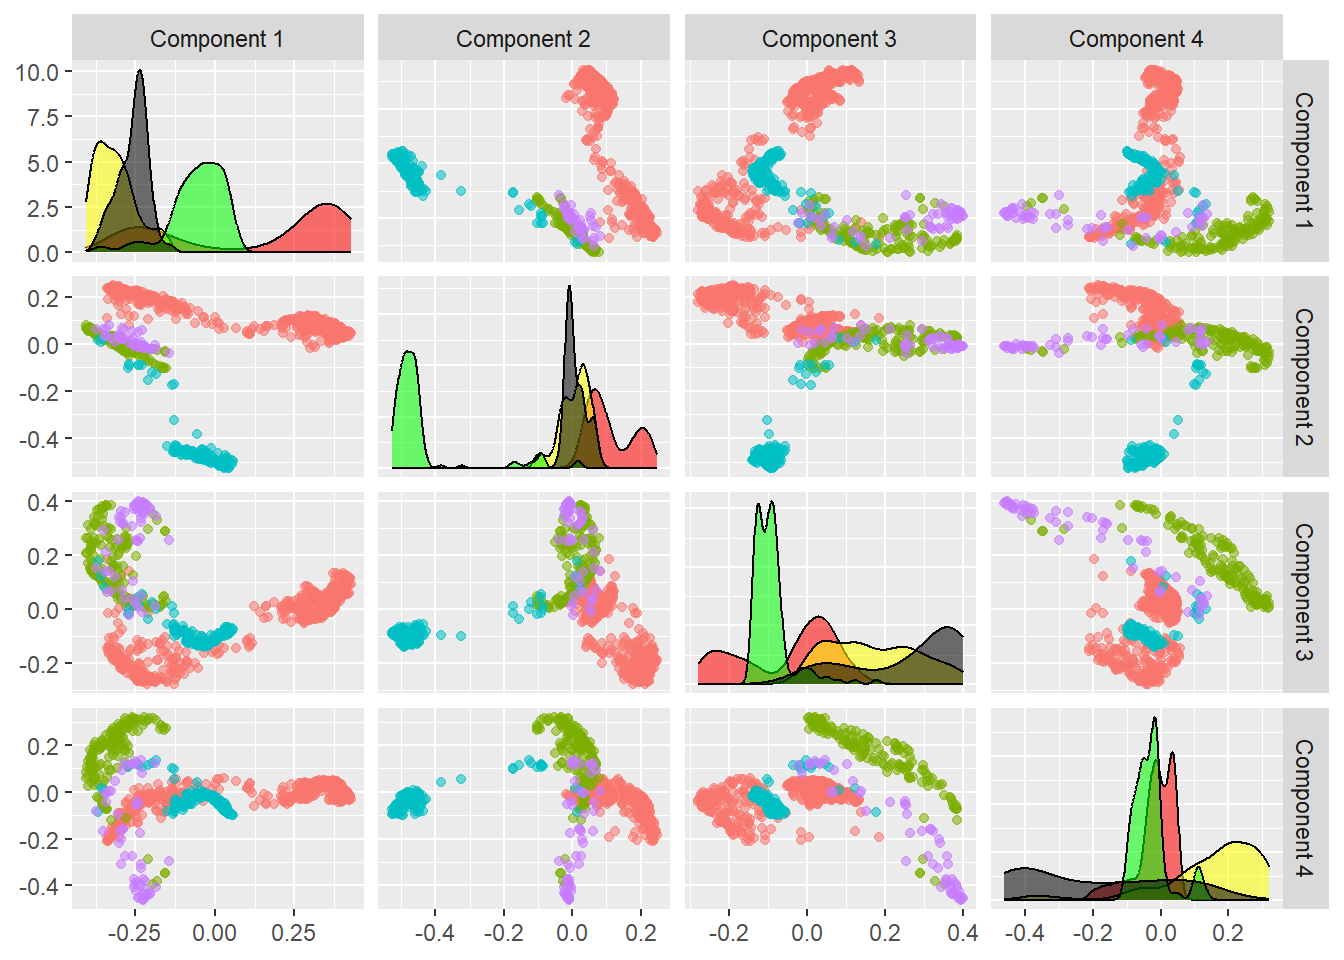
\includegraphics[width=1\textwidth,height=\textheight]{m_DAGs_similarity_files/figure-pdf/unnamed-chunk-25-1.pdf}

\begin{Shaded}
\begin{Highlighting}[]
\NormalTok{sim\_pairs}\OtherTok{=}\NormalTok{ Sim\_comp}\SpecialCharTok{\%\textgreater{}\%} \FunctionTok{pivot\_longer}\NormalTok{(}
  \AttributeTok{cols=}\FunctionTok{c}\NormalTok{(Sim\_MSA,Sim\_Mun),}
  \AttributeTok{names\_to=}\StringTok{"Method"}\NormalTok{,}
  \AttributeTok{values\_to=}\StringTok{"Similarity"}\NormalTok{)}

\NormalTok{ggstatsplot}\SpecialCharTok{::}\FunctionTok{ggbetweenstats}\NormalTok{(}
  \AttributeTok{data =}\NormalTok{ sim\_pairs,}
  \AttributeTok{x =}\NormalTok{ Method,}
  \AttributeTok{y =}\NormalTok{ Similarity,}
  \AttributeTok{centrality.plotting=}\ConstantTok{TRUE}\NormalTok{)}
\end{Highlighting}
\end{Shaded}

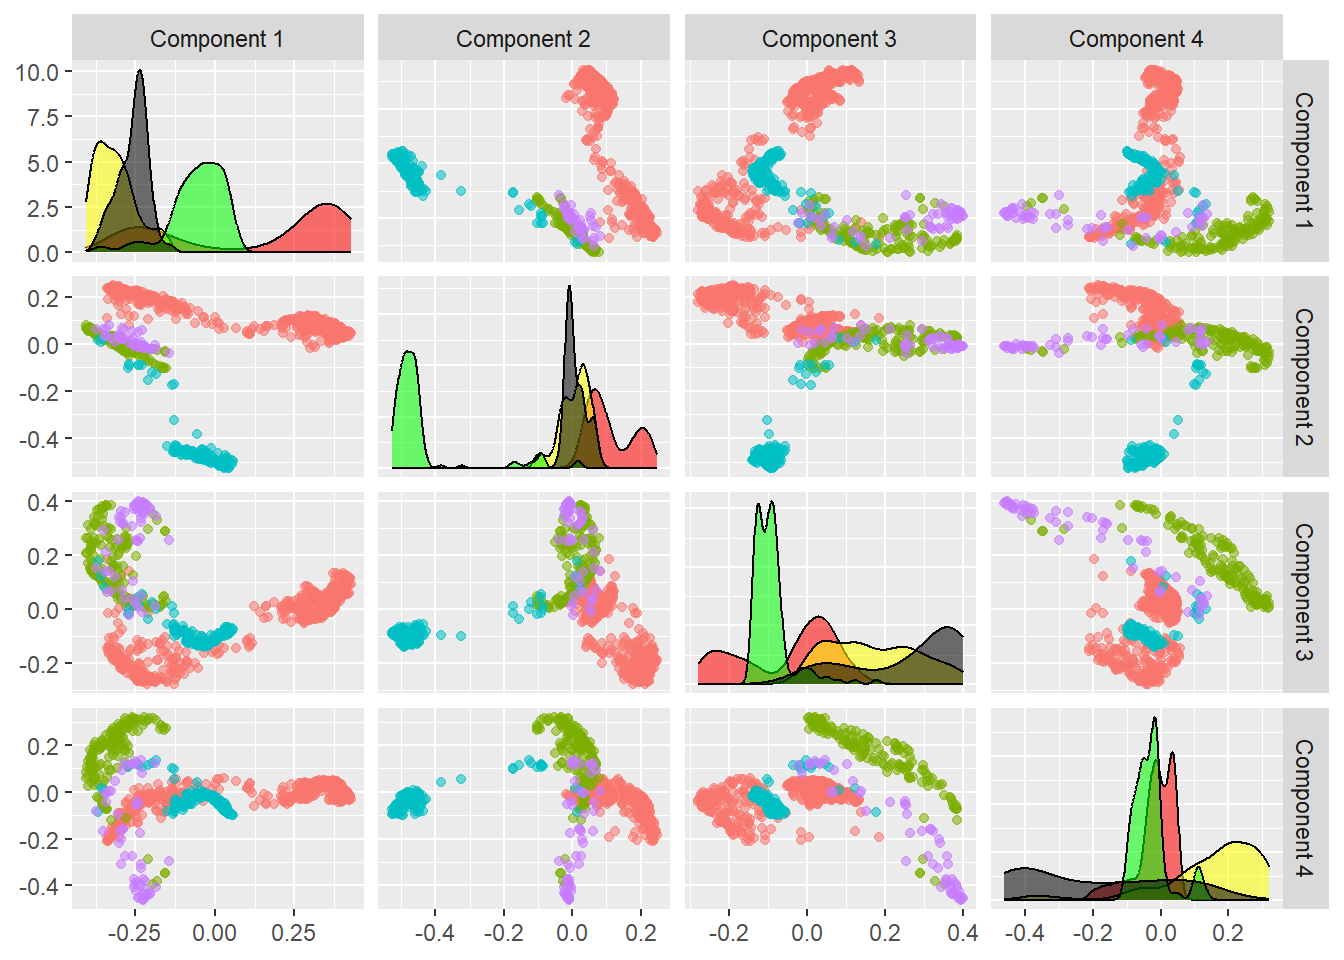
\includegraphics[width=1\textwidth,height=\textheight]{m_DAGs_similarity_files/figure-pdf/unnamed-chunk-26-1.pdf}

\begin{Shaded}
\begin{Highlighting}[]
\FunctionTok{library}\NormalTok{(hrbrthemes)}
\FunctionTok{library}\NormalTok{(viridis)}
\NormalTok{sim\_pairs }\SpecialCharTok{\%\textgreater{}\%}
  \FunctionTok{ggplot}\NormalTok{( }\FunctionTok{aes}\NormalTok{(}\AttributeTok{x=}\NormalTok{Method, }\AttributeTok{y=}\NormalTok{Similarity, }\AttributeTok{fill=}\NormalTok{Method)) }\SpecialCharTok{+}
  \FunctionTok{geom\_boxplot}\NormalTok{() }\SpecialCharTok{+}
  \FunctionTok{scale\_fill\_viridis}\NormalTok{(}\AttributeTok{discrete =} \ConstantTok{TRUE}\NormalTok{, }\AttributeTok{alpha=}\FloatTok{0.6}\NormalTok{) }\SpecialCharTok{+}
  \FunctionTok{theme}\NormalTok{(}\AttributeTok{legend.position=}\StringTok{"none"}\NormalTok{)}\SpecialCharTok{+}
  \FunctionTok{ggtitle}\NormalTok{(}\StringTok{"Boxplot diagram of the similarities between the two aproaches"}\NormalTok{) }
\end{Highlighting}
\end{Shaded}

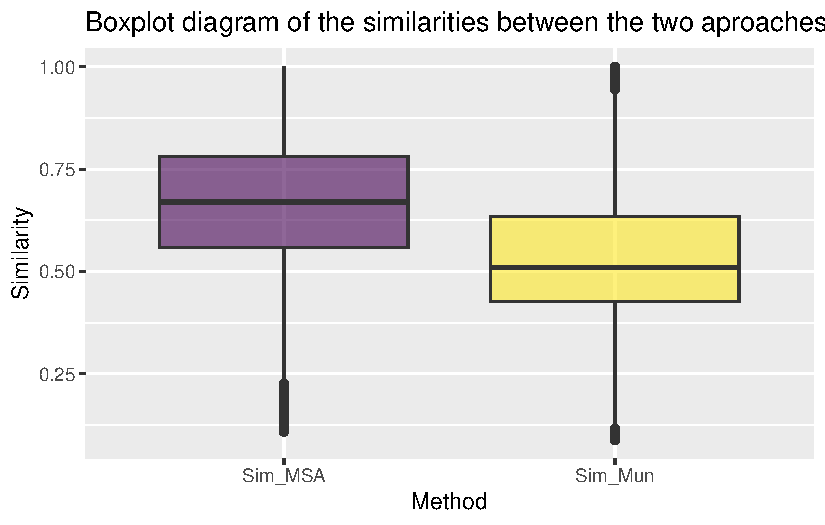
\includegraphics[width=1\textwidth,height=\textheight]{m_DAGs_similarity_files/figure-pdf/unnamed-chunk-27-1.pdf}

Basic statistics similarity

\begin{Shaded}
\begin{Highlighting}[]
\NormalTok{sim\_pairs }\SpecialCharTok{\%\textgreater{}\%} \FunctionTok{group\_by}\NormalTok{(Method) }\SpecialCharTok{\%\textgreater{}\%} 
  \FunctionTok{summarise}\NormalTok{(}\AttributeTok{N=}\FunctionTok{n}\NormalTok{(),}
          \AttributeTok{mean=}\FunctionTok{mean}\NormalTok{(Similarity),}
          \AttributeTok{sd=}\FunctionTok{sd}\NormalTok{(Similarity),}
          \AttributeTok{Q1=}\FunctionTok{quantile}\NormalTok{(Similarity,}\FloatTok{0.25}\NormalTok{),}
          \AttributeTok{median=}\FunctionTok{quantile}\NormalTok{(Similarity,}\FloatTok{0.5}\NormalTok{),}
          \AttributeTok{Q3=}\FunctionTok{quantile}\NormalTok{(Similarity,}\FloatTok{0.75}\NormalTok{))}
\end{Highlighting}
\end{Shaded}

\begin{verbatim}
# A tibble: 2 x 7
  Method       N  mean    sd    Q1 median    Q3
  <chr>    <int> <dbl> <dbl> <dbl>  <dbl> <dbl>
1 Sim_MSA 390286 0.672 0.182 0.559  0.670 0.781
2 Sim_Mun 390286 0.547 0.202 0.427  0.509 0.635
\end{verbatim}

\bookmarksetup{startatroot}

\chapter{Clusters analysis}\label{clusters-analysis}

\begin{Shaded}
\begin{Highlighting}[]
\FunctionTok{load}\NormalTok{(}\AttributeTok{file=}\StringTok{\textquotesingle{}metadag\_work\_space.RData\textquotesingle{}}\NormalTok{)}
\end{Highlighting}
\end{Shaded}

In the Eukaryotes test, we aimed to analyze which factors caused some
algae and plants to be distinguished from their respective kingdoms. To
address this question, we revisited the core metabolism obtained with
MetaDAG, focusing on each cluster.

\begin{Shaded}
\begin{Highlighting}[]
\NormalTok{reactions}\OtherTok{=}\FunctionTok{names}\NormalTok{(Results)}
\NormalTok{reactions}\OtherTok{=}\NormalTok{reactions[}\FunctionTok{grep}\NormalTok{(}\StringTok{"(\^{}R}\SpecialCharTok{\textbackslash{}\textbackslash{}}\StringTok{d\{5\})"}\NormalTok{,reactions)]}
\NormalTok{reactions}\OtherTok{=}\FunctionTok{tibble}\NormalTok{(reactions)}
\NormalTok{reactions}\OtherTok{=}\NormalTok{reactions }\SpecialCharTok{\%\textgreater{}\%} \FunctionTok{separate}\NormalTok{(reactions, }\AttributeTok{into=}\FunctionTok{c}\NormalTok{(}\StringTok{"r\_id"}\NormalTok{,}\StringTok{"enzyme"}\NormalTok{),}\AttributeTok{sep=}\StringTok{"}\SpecialCharTok{\textbackslash{}\textbackslash{}}\StringTok{("}\NormalTok{,}\AttributeTok{remove=}\ConstantTok{FALSE}\NormalTok{)}
\NormalTok{reactions}\OtherTok{=}\NormalTok{reactions }\SpecialCharTok{\%\textgreater{}\%} \FunctionTok{mutate}\NormalTok{(}\AttributeTok{enzyme=}\FunctionTok{gsub}\NormalTok{(}\StringTok{"}\SpecialCharTok{\textbackslash{}\textbackslash{}}\StringTok{(|}\SpecialCharTok{\textbackslash{}\textbackslash{}}\StringTok{)"}\NormalTok{,}\StringTok{""}\NormalTok{,enzyme))}
\CommentTok{\#reactions=reactions[,{-}3]}
\NormalTok{reactions}\SpecialCharTok{$}\NormalTok{rev}\OtherTok{=}\NormalTok{stringr}\SpecialCharTok{::}\FunctionTok{str\_detect}\NormalTok{(reactions}\SpecialCharTok{$}\NormalTok{r\_id,}\StringTok{"v"}\NormalTok{)}
\end{Highlighting}
\end{Shaded}

The results of the clusters are compared to the classification of
Kingdoms for both similarity measures:

\begin{Shaded}
\begin{Highlighting}[]
\NormalTok{clust4\_MSA2}\OtherTok{=}\FunctionTok{tibble}\NormalTok{(}\AttributeTok{mDAG\_Id=}\FunctionTok{names}\NormalTok{(clust4\_MSA), }\AttributeTok{clust4\_MSA=}\NormalTok{clust4\_MSA)}
\NormalTok{clust4\_Mun2}\OtherTok{=}\FunctionTok{tibble}\NormalTok{(}\AttributeTok{mDAG\_Id=}\FunctionTok{names}\NormalTok{(clust4\_Mun), }\AttributeTok{clust4\_Mun=}\NormalTok{clust4\_Mun)}
\NormalTok{meta\_taxo2}\OtherTok{=}\NormalTok{meta\_taxo}
\NormalTok{meta\_taxo2}\OtherTok{=}\NormalTok{meta\_taxo2 }\SpecialCharTok{\%\textgreater{}\%} \FunctionTok{left\_join}\NormalTok{(clust4\_MSA2,}\AttributeTok{by=} \StringTok{"mDAG\_Id"}\NormalTok{) }\SpecialCharTok{\%\textgreater{}\%} 
  \FunctionTok{left\_join}\NormalTok{(clust4\_Mun2,}\AttributeTok{by=} \StringTok{"mDAG\_Id"}\NormalTok{)}
\NormalTok{meta\_taxo2}\SpecialCharTok{$}\NormalTok{combined\_cluster\_MSA\_Kingdom}\OtherTok{=}\FunctionTok{paste0}\NormalTok{(meta\_taxo2}\SpecialCharTok{$}\NormalTok{Kingdom,meta\_taxo2}\SpecialCharTok{$}\NormalTok{clust4\_MSA)}
\NormalTok{meta\_taxo2}\SpecialCharTok{$}\NormalTok{combined\_cluster\_Mun\_Kingdom}\OtherTok{=}\FunctionTok{paste0}\NormalTok{(meta\_taxo2}\SpecialCharTok{$}\NormalTok{Kingdom,meta\_taxo2}\SpecialCharTok{$}\NormalTok{clust4\_MSA)}
\FunctionTok{write.csv}\NormalTok{(meta\_taxo2,}\AttributeTok{file=}\StringTok{"meta\_taxo\_4\_clusters.csv"}\NormalTok{)}
\end{Highlighting}
\end{Shaded}

\begin{Shaded}
\begin{Highlighting}[]
\NormalTok{knitr}\SpecialCharTok{::}\FunctionTok{kable}\NormalTok{(}\FunctionTok{table}\NormalTok{(meta\_taxo2}\SpecialCharTok{$}\NormalTok{Kingdom,meta\_taxo2}\SpecialCharTok{$}\NormalTok{clust4\_MSA))}
\end{Highlighting}
\end{Shaded}

\begin{longtable}[]{@{}lrrrr@{}}
\toprule\noalign{}
& 1 & 2 & 3 & 4 \\
\midrule\noalign{}
\endhead
\bottomrule\noalign{}
\endlastfoot
Animals & 331 & 197 & 7 & 0 \\
Fungi & 0 & 0 & 154 & 0 \\
Plants & 0 & 0 & 14 & 125 \\
Protists & 0 & 0 & 56 & 0 \\
\end{longtable}

\begin{Shaded}
\begin{Highlighting}[]
\NormalTok{knitr}\SpecialCharTok{::}\FunctionTok{kable}\NormalTok{(}\FunctionTok{table}\NormalTok{(meta\_taxo2}\SpecialCharTok{$}\NormalTok{Kingdom,meta\_taxo2}\SpecialCharTok{$}\NormalTok{clust4\_Mun))}
\end{Highlighting}
\end{Shaded}

\begin{longtable}[]{@{}lrrrr@{}}
\toprule\noalign{}
& 1 & 2 & 3 & 4 \\
\midrule\noalign{}
\endhead
\bottomrule\noalign{}
\endlastfoot
Animals & 331 & 197 & 7 & 0 \\
Fungi & 0 & 0 & 154 & 0 \\
Plants & 0 & 0 & 14 & 125 \\
Protists & 0 & 0 & 56 & 0 \\
\end{longtable}

\begin{Shaded}
\begin{Highlighting}[]
\NormalTok{knitr}\SpecialCharTok{::}\FunctionTok{kable}\NormalTok{(}\FunctionTok{table}\NormalTok{(meta\_taxo2}\SpecialCharTok{$}\NormalTok{clust4\_Mun,meta\_taxo2}\SpecialCharTok{$}\NormalTok{clust4\_MSA))}
\end{Highlighting}
\end{Shaded}

\begin{longtable}[]{@{}rrrr@{}}
\toprule\noalign{}
1 & 2 & 3 & 4 \\
\midrule\noalign{}
\endhead
\bottomrule\noalign{}
\endlastfoot
331 & 0 & 0 & 0 \\
0 & 197 & 0 & 0 \\
0 & 0 & 231 & 0 \\
0 & 0 & 0 & 125 \\
\end{longtable}

The table below correlates the clusters with the Phylum information.

\begin{Shaded}
\begin{Highlighting}[]
\FunctionTok{library}\NormalTok{(reshape2)}
\NormalTok{MSA\_table}\OtherTok{=}\FunctionTok{melt}\NormalTok{(}\FunctionTok{table}\NormalTok{(meta\_taxo2}\SpecialCharTok{$}\NormalTok{Kingdom,meta\_taxo2}\SpecialCharTok{$}\NormalTok{Phylum,meta\_taxo2}\SpecialCharTok{$}\NormalTok{clust4\_MSA))}
\FunctionTok{names}\NormalTok{(MSA\_table)}\OtherTok{=}\FunctionTok{c}\NormalTok{(}\StringTok{"Kingdom"}\NormalTok{,}\StringTok{"Phylum"}\NormalTok{,}\StringTok{"cluster\_MSA"}\NormalTok{,}\StringTok{"N"}\NormalTok{)}
\NormalTok{MSA\_table}\OtherTok{=}\NormalTok{MSA\_table }\SpecialCharTok{\%\textgreater{}\%} \FunctionTok{filter}\NormalTok{(N}\SpecialCharTok{!=}\DecValTok{0}\NormalTok{)}
\end{Highlighting}
\end{Shaded}

\begin{Shaded}
\begin{Highlighting}[]
\NormalTok{knitr}\SpecialCharTok{::}\FunctionTok{kable}\NormalTok{(MSA\_table)}
\end{Highlighting}
\end{Shaded}

\begin{longtable}[]{@{}llrr@{}}
\toprule\noalign{}
Kingdom & Phylum & cluster\_MSA & N \\
\midrule\noalign{}
\endhead
\bottomrule\noalign{}
\endlastfoot
Animals & Vertebrates & 1 & 331 \\
Animals & Annelids & 2 & 1 \\
Animals & Arthropods & 2 & 158 \\
Animals & Brachiopodas & 2 & 1 \\
Animals & Cephalochordates & 2 & 2 \\
Animals & Cnidarians & 2 & 10 \\
Animals & Echinoderms & 2 & 3 \\
Animals & Hemichordates & 2 & 1 \\
Animals & Mollusks & 2 & 14 \\
Animals & Nematodes & 2 & 3 \\
Animals & Placozoans & 2 & 1 \\
Animals & Poriferans & 2 & 1 \\
Animals & Tunicates & 2 & 2 \\
Protists & Alveolates & 3 & 25 \\
Protists & Amoebozoa & 3 & 7 \\
Fungi & Ascomycetes & 3 & 113 \\
Fungi & Basidiomycetes & 3 & 36 \\
Protists & Choanoflagellates & 3 & 2 \\
Protists & Cryptomonads & 3 & 1 \\
Protists & Euglenozoa & 3 & 9 \\
Animals & Flatworms & 3 & 4 \\
Plants & Green & 3 & 11 \\
Protists & Haptophyta & 3 & 1 \\
Protists & Heterolobosea & 3 & 1 \\
Protists & Metamonada & 3 & 2 \\
Fungi & Microsporidians & 3 & 5 \\
Animals & Nematodes & 3 & 3 \\
Plants & Red & 3 & 3 \\
Protists & Stramenopiles & 3 & 8 \\
Plants & Basal & 4 & 2 \\
Plants & Eudicots & 4 & 98 \\
Plants & Ferns & 4 & 1 \\
Plants & Monocots & 4 & 23 \\
Plants & Mosses & 4 & 1 \\
\end{longtable}

\bookmarksetup{startatroot}

\chapter{Appendix}\label{appendix}

Some tables and graphs for the supplementary material.

\begin{Shaded}
\begin{Highlighting}[]
\FunctionTok{load}\NormalTok{(}\AttributeTok{file=}\StringTok{\textquotesingle{}metadag\_work\_space.RData\textquotesingle{}}\NormalTok{)}
\end{Highlighting}
\end{Shaded}

Table MBB sizes

\begin{Shaded}
\begin{Highlighting}[]
\NormalTok{write\_delim}\OtherTok{=}\FunctionTok{write\_delim}\NormalTok{(table\_MBB\_size,}
                        \AttributeTok{file=}\StringTok{"data\_appendix/table\_MBB\_size.csv"}\NormalTok{,}
                        \AttributeTok{delim=}\StringTok{","}\NormalTok{)}
\end{Highlighting}
\end{Shaded}

\begin{Shaded}
\begin{Highlighting}[]
\NormalTok{clust4\_MSA2}\OtherTok{=}\FunctionTok{tibble}\NormalTok{(}\AttributeTok{mDAG\_Id=}\FunctionTok{names}\NormalTok{(clust4\_MSA),}
                      \AttributeTok{clust4\_MSA=}\FunctionTok{as.integer}\NormalTok{(clust4\_MSA))}
\NormalTok{clust4\_Mun2}\OtherTok{=}\FunctionTok{tibble}\NormalTok{(}\AttributeTok{mDAG\_Id=}\FunctionTok{names}\NormalTok{(clust4\_Mun),}
                      \AttributeTok{clust4\_Mun=}\FunctionTok{as.integer}\NormalTok{(clust4\_Mun))}

\NormalTok{clust4\_MSA\_Eukaryotes\_taxo}\OtherTok{=}\NormalTok{ meta\_taxo }\SpecialCharTok{\%\textgreater{}\%} \FunctionTok{filter}\NormalTok{(}\SpecialCharTok{!}\FunctionTok{is.na}\NormalTok{(Kingdom))}\SpecialCharTok{\%\textgreater{}\%}
  \FunctionTok{select}\NormalTok{(}\SpecialCharTok{{-}}\FunctionTok{c}\NormalTok{(Freq\_Kingdom,Freq\_Phylum,Freq\_Class)) }\SpecialCharTok{\%\textgreater{}\%}
  \FunctionTok{left\_join}\NormalTok{(clust4\_MSA2,}\AttributeTok{by=}\StringTok{"mDAG\_Id"}\NormalTok{)}
  
\NormalTok{clust4\_Mun\_Eukaryotes\_taxo}\OtherTok{=}\NormalTok{ meta\_taxo }\SpecialCharTok{\%\textgreater{}\%} \FunctionTok{filter}\NormalTok{(}\SpecialCharTok{!}\FunctionTok{is.na}\NormalTok{(Kingdom))}\SpecialCharTok{\%\textgreater{}\%}
  \FunctionTok{select}\NormalTok{(}\SpecialCharTok{{-}}\FunctionTok{c}\NormalTok{(Freq\_Kingdom,Freq\_Phylum,Freq\_Class)) }\SpecialCharTok{\%\textgreater{}\%}
  \FunctionTok{left\_join}\NormalTok{(clust4\_Mun2,}\AttributeTok{by=}\StringTok{"mDAG\_Id"}\NormalTok{)}
  



\FunctionTok{write\_delim}\NormalTok{(clust4\_MSA\_Eukaryotes\_taxo,}
                        \AttributeTok{file=}\StringTok{"data\_appendix/clust4\_MSA\_Eukaryotes\_taxo.csv"}\NormalTok{,}
                        \AttributeTok{delim=}\StringTok{","}\NormalTok{)}
\FunctionTok{write\_delim}\NormalTok{(clust4\_Mun\_Eukaryotes\_taxo,}
                        \AttributeTok{file=}\StringTok{"data\_appendix/clust4\_Mun\_Eukaryotes\_taxo.csv"}\NormalTok{,}
                        \AttributeTok{delim=}\StringTok{","}\NormalTok{)}
\end{Highlighting}
\end{Shaded}

Heatmaps by Kingdom MSA y Mun: Animals, Fungi, Plants ans Protists.

\textbf{Animals}

\begin{Shaded}
\begin{Highlighting}[]
\DocumentationTok{\#\#  Animals by phylum}
\NormalTok{meta\_animals}\OtherTok{=}\NormalTok{ meta\_taxo }\SpecialCharTok{\%\textgreater{}\%} \FunctionTok{filter}\NormalTok{(Kingdom}\SpecialCharTok{==}\StringTok{"Animals"}\NormalTok{)}
\NormalTok{namesP}\OtherTok{=}\FunctionTok{names}\NormalTok{(}\FunctionTok{rev}\NormalTok{(}\FunctionTok{sort}\NormalTok{(}\FunctionTok{table}\NormalTok{(meta\_animals}\SpecialCharTok{$}\NormalTok{Phylum))))}
\NormalTok{namesP}
\end{Highlighting}
\end{Shaded}

\begin{verbatim}
 [1] "Vertebrates"      "Arthropods"       "Mollusks"         "Cnidarians"      
 [5] "Nematodes"        "Flatworms"        "Echinoderms"      "Tunicates"       
 [9] "Cephalochordates" "Poriferans"       "Placozoans"       "Hemichordates"   
[13] "Brachiopodas"     "Annelids"        
\end{verbatim}

\begin{Shaded}
\begin{Highlighting}[]
\NormalTok{dff}\OtherTok{=}\FunctionTok{data.frame}\NormalTok{(}\AttributeTok{Phylum=}\NormalTok{meta\_animals}\SpecialCharTok{$}\NormalTok{Phylum)}
\NormalTok{Phylum}\OtherTok{=}\FunctionTok{ordered}\NormalTok{(meta\_animals}\SpecialCharTok{$}\NormalTok{Phylum,}\AttributeTok{levels=}\NormalTok{namesP)}
\NormalTok{numbersP}\OtherTok{=}\FunctionTok{paste}\NormalTok{(}\FunctionTok{c}\NormalTok{(}\FunctionTok{paste0}\NormalTok{(}\DecValTok{0}\NormalTok{,}\DecValTok{1}\SpecialCharTok{:}\DecValTok{9}\NormalTok{),}\DecValTok{10}\SpecialCharTok{:}\DecValTok{14}\NormalTok{),namesP,}\AttributeTok{sep=}\StringTok{"{-}"}\NormalTok{)}
\FunctionTok{levels}\NormalTok{(Phylum)}\OtherTok{=}\NormalTok{numbersP}
\NormalTok{dff}\SpecialCharTok{$}\NormalTok{Phylum}\OtherTok{=}\NormalTok{Phylum}
\NormalTok{col}\OtherTok{=}\FunctionTok{rainbow}\NormalTok{(}\FunctionTok{length}\NormalTok{(namesP))}

\NormalTok{colorsP}\OtherTok{=}\FunctionTok{list}\NormalTok{(}\AttributeTok{Phylum=}\NormalTok{col)}
\FunctionTok{names}\NormalTok{(colorsP}\SpecialCharTok{$}\NormalTok{Phylum)}\OtherTok{=}\NormalTok{numbersP}

\NormalTok{annot }\OtherTok{\textless{}{-}} \FunctionTok{HeatmapAnnotation}\NormalTok{(}\AttributeTok{df =}\NormalTok{ dff, }
                               \AttributeTok{col =}\NormalTok{ colorsP,}
                               \AttributeTok{annotation\_name\_side =} \StringTok{"left"}\NormalTok{,}
                               \AttributeTok{show\_annotation\_name=}\ConstantTok{TRUE}\NormalTok{ )}

\NormalTok{MSA\_heat\_2 }\OtherTok{\textless{}{-}}  \FunctionTok{Heatmap}\NormalTok{(}
  \AttributeTok{matrix =}\NormalTok{ Sim\_MSA\_mDAG[meta\_animals}\SpecialCharTok{$}\NormalTok{mDAG\_Id,}
\NormalTok{                        meta\_animals}\SpecialCharTok{$}\NormalTok{mDAG\_Id],}
  \AttributeTok{name =} \StringTok{"MSA similarity"}\NormalTok{,}
  \AttributeTok{column\_title =} \StringTok{"m{-}DAGs MSA{-}similarity  Animals by Phyla"}\NormalTok{,}
  \AttributeTok{col =} \FunctionTok{rev}\NormalTok{(}\FunctionTok{viridis}\NormalTok{(}\DecValTok{256}\NormalTok{)),}
  \AttributeTok{cluster\_rows =} \ConstantTok{FALSE}\NormalTok{,}
  \AttributeTok{show\_heatmap\_legend =} \ConstantTok{FALSE}\NormalTok{,}
  \AttributeTok{cluster\_columns =} \ConstantTok{FALSE}\NormalTok{,}
  \AttributeTok{top\_annotation =}\NormalTok{ annot,}
  \AttributeTok{show\_column\_names =} \ConstantTok{FALSE}\NormalTok{,}
  \AttributeTok{show\_row\_names =} \ConstantTok{FALSE}\NormalTok{,}
  \AttributeTok{left\_annotation =}
    \FunctionTok{rowAnnotation}\NormalTok{(}
      \AttributeTok{df =}\NormalTok{ dff,}
      \AttributeTok{col =}\NormalTok{ colorsP,}
      \AttributeTok{show\_annotation\_name =} \ConstantTok{FALSE}
\NormalTok{    )}
\NormalTok{)}




\NormalTok{Mun\_heat\_2 }\OtherTok{\textless{}{-}} \FunctionTok{Heatmap}\NormalTok{(}
  \AttributeTok{matrix =}\NormalTok{ Sim\_Mun\_mDAG[meta\_animals}\SpecialCharTok{$}\NormalTok{mDAG\_Id,}
\NormalTok{                        meta\_animals}\SpecialCharTok{$}\NormalTok{mDAG\_Id],}
  \AttributeTok{column\_title =} \StringTok{"m{-}DAGs Munkres{-}similarity  Animals by Phyla"}\NormalTok{,}
 \AttributeTok{col =} \FunctionTok{rev}\NormalTok{(}\FunctionTok{viridis}\NormalTok{(}\DecValTok{256}\NormalTok{)),}
  \AttributeTok{cluster\_rows =} \ConstantTok{FALSE}\NormalTok{,}
  \AttributeTok{show\_heatmap\_legend =} \ConstantTok{FALSE}\NormalTok{,}
  \AttributeTok{cluster\_columns =} \ConstantTok{FALSE}\NormalTok{,}
  \AttributeTok{top\_annotation =}\NormalTok{ annot,}
  \AttributeTok{show\_column\_names =} \ConstantTok{FALSE}\NormalTok{,}
  \AttributeTok{show\_row\_names =} \ConstantTok{FALSE}\NormalTok{,}
  \AttributeTok{left\_annotation =}
    \FunctionTok{rowAnnotation}\NormalTok{(}
      \AttributeTok{df =}\NormalTok{ dff,}
      \AttributeTok{col =}\NormalTok{ colorsP,}
      \AttributeTok{show\_annotation\_name =} \ConstantTok{FALSE}
\NormalTok{    )}
\NormalTok{)}
\end{Highlighting}
\end{Shaded}

Save graphics

\begin{verbatim}
pdf 
  2 
\end{verbatim}

\begin{verbatim}
pdf 
  2 
\end{verbatim}

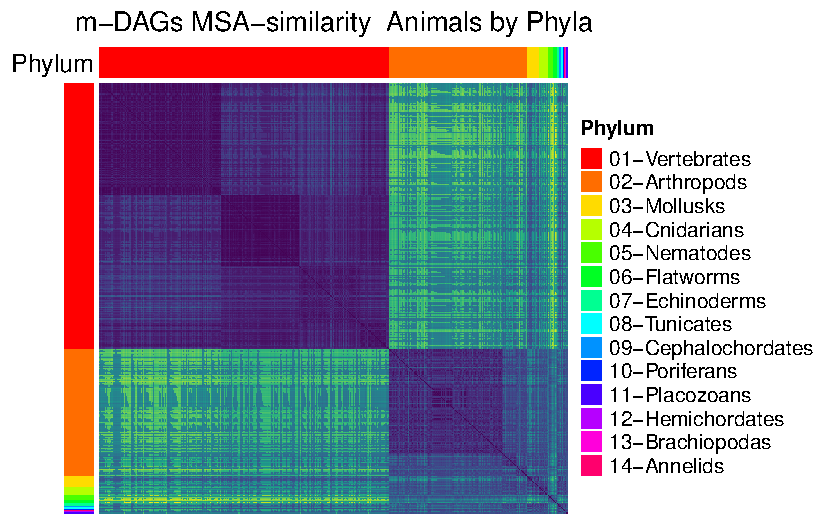
\includegraphics[width=1\textwidth,height=\textheight]{appendix_files/figure-pdf/unnamed-chunk-7-1.pdf}

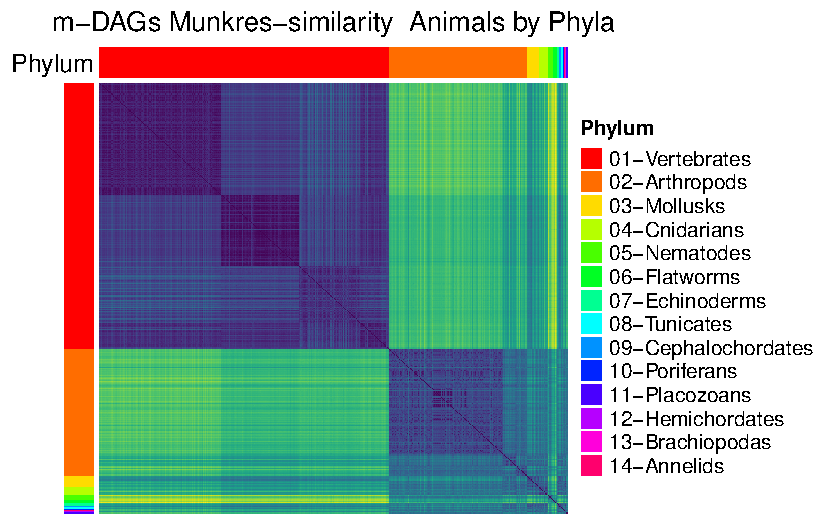
\includegraphics[width=1\textwidth,height=\textheight]{appendix_files/figure-pdf/unnamed-chunk-7-2.pdf}

\textbf{Plants}

\begin{Shaded}
\begin{Highlighting}[]
\NormalTok{meta\_plants}\OtherTok{=}\NormalTok{ meta\_taxo[}\DecValTok{1}\SpecialCharTok{:}\DecValTok{884}\NormalTok{,] }\SpecialCharTok{\%\textgreater{}\%} \FunctionTok{filter}\NormalTok{(Kingdom}\SpecialCharTok{==}\StringTok{"Plants"}\NormalTok{)}
\NormalTok{namesP}\OtherTok{=}\FunctionTok{names}\NormalTok{(}\FunctionTok{rev}\NormalTok{(}\FunctionTok{sort}\NormalTok{(}\FunctionTok{table}\NormalTok{(meta\_plants}\SpecialCharTok{$}\NormalTok{Phylum))))}
\NormalTok{namesP}
\end{Highlighting}
\end{Shaded}

\begin{verbatim}
[1] "Eudicots" "Monocots" "Green"    "Red"      "Basal"    "Mosses"   "Ferns"   
\end{verbatim}

\begin{Shaded}
\begin{Highlighting}[]
\NormalTok{dff}\OtherTok{=}\FunctionTok{data.frame}\NormalTok{(}\AttributeTok{Phylum=}\NormalTok{meta\_plants}\SpecialCharTok{$}\NormalTok{Phylum)}
\NormalTok{Phylum}\OtherTok{=}\FunctionTok{ordered}\NormalTok{(meta\_plants}\SpecialCharTok{$}\NormalTok{Phylum,}\AttributeTok{levels=}\NormalTok{namesP)}
\NormalTok{numbersP}\OtherTok{=}\FunctionTok{paste}\NormalTok{(}\FunctionTok{c}\NormalTok{(}\FunctionTok{paste0}\NormalTok{(}\DecValTok{0}\NormalTok{,}\DecValTok{1}\SpecialCharTok{:}\DecValTok{7}\NormalTok{)),namesP,}\AttributeTok{sep=}\StringTok{"{-}"}\NormalTok{)}
\FunctionTok{levels}\NormalTok{(Phylum)}\OtherTok{=}\NormalTok{numbersP}
\NormalTok{dff}\SpecialCharTok{$}\NormalTok{Phylum}\OtherTok{=}\NormalTok{Phylum}
\NormalTok{col}\OtherTok{=}\FunctionTok{rainbow}\NormalTok{(}\FunctionTok{length}\NormalTok{(namesP))}

\NormalTok{colorsP}\OtherTok{=}\FunctionTok{list}\NormalTok{(}\AttributeTok{Phylum=}\NormalTok{col)}
\FunctionTok{names}\NormalTok{(colorsP}\SpecialCharTok{$}\NormalTok{Phylum)}\OtherTok{=}\NormalTok{numbersP}

\NormalTok{annot }\OtherTok{\textless{}{-}} \FunctionTok{HeatmapAnnotation}\NormalTok{(}\AttributeTok{df =}\NormalTok{ dff, }
                               \AttributeTok{col =}\NormalTok{ colorsP,}
                               \AttributeTok{annotation\_name\_side =} \StringTok{"left"}\NormalTok{,}
                               \AttributeTok{show\_annotation\_name=}\ConstantTok{TRUE}\NormalTok{ )}

\NormalTok{MSA\_heat\_2 }\OtherTok{\textless{}{-}}  \FunctionTok{Heatmap}\NormalTok{(}
  \AttributeTok{matrix =}\NormalTok{ Sim\_MSA\_mDAG[meta\_plants}\SpecialCharTok{$}\NormalTok{mDAG\_Id,}
\NormalTok{                        meta\_plants}\SpecialCharTok{$}\NormalTok{mDAG\_Id],}
  \AttributeTok{name =} \StringTok{"MSA similarity"}\NormalTok{,}
  \AttributeTok{column\_title =} \StringTok{"m{-}DAGs MSA{-}similarity  Plants by Phyla"}\NormalTok{,}
  \AttributeTok{col =} \FunctionTok{rev}\NormalTok{(}\FunctionTok{viridis}\NormalTok{(}\DecValTok{256}\NormalTok{)),}
  \AttributeTok{cluster\_rows =} \ConstantTok{FALSE}\NormalTok{,}
  \AttributeTok{show\_heatmap\_legend =} \ConstantTok{FALSE}\NormalTok{,}
  \AttributeTok{cluster\_columns =} \ConstantTok{FALSE}\NormalTok{,}
  \AttributeTok{top\_annotation =}\NormalTok{ annot,}
  \AttributeTok{show\_column\_names =} \ConstantTok{FALSE}\NormalTok{,}
  \AttributeTok{show\_row\_names =} \ConstantTok{FALSE}\NormalTok{,}
  \AttributeTok{left\_annotation =}
    \FunctionTok{rowAnnotation}\NormalTok{(}
      \AttributeTok{df =}\NormalTok{ dff,}
      \AttributeTok{col =}\NormalTok{ colorsP,}
      \AttributeTok{show\_annotation\_name =} \ConstantTok{FALSE}
\NormalTok{    )}
\NormalTok{)}

\NormalTok{Mun\_heat\_2 }\OtherTok{\textless{}{-}} \FunctionTok{Heatmap}\NormalTok{(}
  \AttributeTok{matrix =}\NormalTok{ Sim\_Mun\_mDAG[meta\_plants}\SpecialCharTok{$}\NormalTok{mDAG\_Id,}
\NormalTok{                        meta\_plants}\SpecialCharTok{$}\NormalTok{mDAG\_Id],}
    \AttributeTok{name =} \StringTok{"Mun similarity"}\NormalTok{,}
  \AttributeTok{column\_title =} \StringTok{"m{-}DAGs Munkres{-}similarity  Plants by Phyla"}\NormalTok{,}
\AttributeTok{col =} \FunctionTok{rev}\NormalTok{(}\FunctionTok{viridis}\NormalTok{(}\DecValTok{256}\NormalTok{)),}
  \AttributeTok{cluster\_rows =} \ConstantTok{FALSE}\NormalTok{,}
  \AttributeTok{show\_heatmap\_legend =} \ConstantTok{FALSE}\NormalTok{,}
  \AttributeTok{cluster\_columns =} \ConstantTok{FALSE}\NormalTok{,}
  \AttributeTok{top\_annotation =}\NormalTok{ annot,}
  \AttributeTok{show\_column\_names =} \ConstantTok{FALSE}\NormalTok{,}
  \AttributeTok{show\_row\_names =} \ConstantTok{FALSE}\NormalTok{,}
  \AttributeTok{left\_annotation =}
    \FunctionTok{rowAnnotation}\NormalTok{(}
      \AttributeTok{df =}\NormalTok{ dff,}
      \AttributeTok{col =}\NormalTok{ colorsP,}
      \AttributeTok{show\_annotation\_name =} \ConstantTok{FALSE}
\NormalTok{    )}
\NormalTok{)}
\end{Highlighting}
\end{Shaded}

Save graphics

\begin{verbatim}
pdf 
  2 
\end{verbatim}

\begin{verbatim}
pdf 
  2 
\end{verbatim}

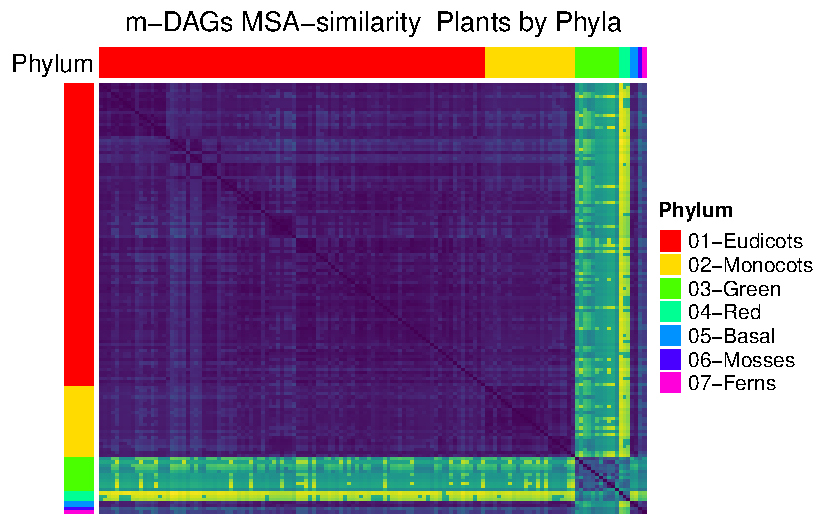
\includegraphics[width=1\textwidth,height=\textheight]{appendix_files/figure-pdf/unnamed-chunk-10-1.pdf}

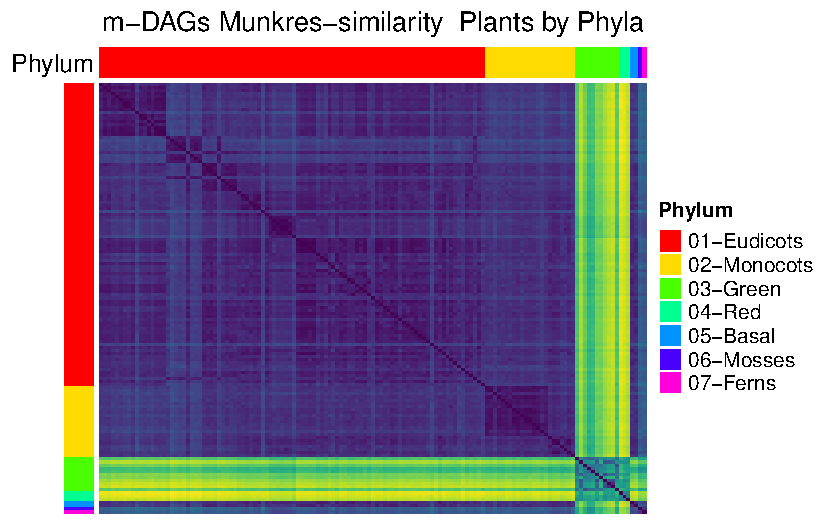
\includegraphics[width=1\textwidth,height=\textheight]{appendix_files/figure-pdf/unnamed-chunk-10-2.pdf}

\textbf{Fungi}

\begin{Shaded}
\begin{Highlighting}[]
\NormalTok{meta\_fungi}\OtherTok{=}\NormalTok{ meta\_taxo}\SpecialCharTok{\%\textgreater{}\%} \FunctionTok{filter}\NormalTok{(Kingdom}\SpecialCharTok{==}\StringTok{"Fungi"}\NormalTok{)}
\NormalTok{namesP}\OtherTok{=}\FunctionTok{names}\NormalTok{(}\FunctionTok{rev}\NormalTok{(}\FunctionTok{sort}\NormalTok{(}\FunctionTok{table}\NormalTok{(meta\_fungi}\SpecialCharTok{$}\NormalTok{Phylum))))}
\NormalTok{namesP}
\end{Highlighting}
\end{Shaded}

\begin{verbatim}
[1] "Ascomycetes"     "Basidiomycetes"  "Microsporidians"
\end{verbatim}

\begin{Shaded}
\begin{Highlighting}[]
\NormalTok{dff}\OtherTok{=}\FunctionTok{data.frame}\NormalTok{(}\AttributeTok{Phylum=}\NormalTok{meta\_fungi}\SpecialCharTok{$}\NormalTok{Phylum)}
\NormalTok{Phylum}\OtherTok{=}\FunctionTok{ordered}\NormalTok{(meta\_fungi}\SpecialCharTok{$}\NormalTok{Phylum,}\AttributeTok{levels=}\NormalTok{namesP)}
\NormalTok{n}\OtherTok{=}\FunctionTok{length}\NormalTok{(namesP)}

\NormalTok{numbersP}\OtherTok{=}\FunctionTok{paste}\NormalTok{(}\FunctionTok{c}\NormalTok{(}\FunctionTok{paste0}\NormalTok{(}\DecValTok{0}\NormalTok{,}\DecValTok{1}\SpecialCharTok{:}\NormalTok{n)),namesP,}\AttributeTok{sep=}\StringTok{"{-}"}\NormalTok{)}
\FunctionTok{levels}\NormalTok{(Phylum)}\OtherTok{=}\NormalTok{numbersP}
\NormalTok{dff}\SpecialCharTok{$}\NormalTok{Phylum}\OtherTok{=}\NormalTok{Phylum}
\NormalTok{col}\OtherTok{=}\FunctionTok{rainbow}\NormalTok{(}\FunctionTok{length}\NormalTok{(namesP))}

\NormalTok{colorsP}\OtherTok{=}\FunctionTok{list}\NormalTok{(}\AttributeTok{Phylum=}\NormalTok{col)}
\FunctionTok{names}\NormalTok{(colorsP}\SpecialCharTok{$}\NormalTok{Phylum)}\OtherTok{=}\NormalTok{numbersP}

\NormalTok{annot }\OtherTok{\textless{}{-}} \FunctionTok{HeatmapAnnotation}\NormalTok{(}\AttributeTok{df =}\NormalTok{ dff, }
                               \AttributeTok{col =}\NormalTok{ colorsP,}
                               \AttributeTok{annotation\_name\_side =} \StringTok{"left"}\NormalTok{,}
                               \AttributeTok{show\_annotation\_name=}\ConstantTok{TRUE}\NormalTok{ )}

\NormalTok{MSA\_heat\_2 }\OtherTok{\textless{}{-}}  \FunctionTok{Heatmap}\NormalTok{(}
  \AttributeTok{matrix =}\NormalTok{ Sim\_MSA\_mDAG[meta\_fungi}\SpecialCharTok{$}\NormalTok{mDAG\_Id,}
\NormalTok{                        meta\_fungi}\SpecialCharTok{$}\NormalTok{mDAG\_Id],}
  \AttributeTok{name =} \StringTok{"MSA similarity"}\NormalTok{,}
  \AttributeTok{column\_title =} \StringTok{"m{-}DAGs MSA{-}similarity  Fungi by Phyla"}\NormalTok{,}
  \AttributeTok{col =} \FunctionTok{rev}\NormalTok{(}\FunctionTok{viridis}\NormalTok{(}\DecValTok{256}\NormalTok{)),}
  \AttributeTok{cluster\_rows =} \ConstantTok{FALSE}\NormalTok{,}
  \AttributeTok{show\_heatmap\_legend =} \ConstantTok{FALSE}\NormalTok{,}
  \AttributeTok{cluster\_columns =} \ConstantTok{FALSE}\NormalTok{,}
  \AttributeTok{top\_annotation =}\NormalTok{ annot,}
  \AttributeTok{show\_column\_names =} \ConstantTok{FALSE}\NormalTok{,}
  \AttributeTok{show\_row\_names =} \ConstantTok{FALSE}\NormalTok{,}
  \AttributeTok{left\_annotation =}
    \FunctionTok{rowAnnotation}\NormalTok{(}
      \AttributeTok{df =}\NormalTok{ dff,}
      \AttributeTok{col =}\NormalTok{ colorsP,}
      \AttributeTok{show\_annotation\_name =} \ConstantTok{FALSE}
\NormalTok{    )}
\NormalTok{)}

\NormalTok{Mun\_heat\_2 }\OtherTok{\textless{}{-}} \FunctionTok{Heatmap}\NormalTok{(}
  \AttributeTok{matrix =}\NormalTok{ Sim\_Mun\_mDAG[meta\_fungi}\SpecialCharTok{$}\NormalTok{mDAG\_Id,}
\NormalTok{                        meta\_fungi}\SpecialCharTok{$}\NormalTok{mDAG\_Id],}
    \AttributeTok{name =} \StringTok{"Mun similarity"}\NormalTok{,}
  \AttributeTok{column\_title =} \StringTok{"m{-}DAGs Munkres{-}similarity  Fungi by Phyla"}\NormalTok{,}
\AttributeTok{col =} \FunctionTok{rev}\NormalTok{(}\FunctionTok{viridis}\NormalTok{(}\DecValTok{256}\NormalTok{)),}
  \AttributeTok{cluster\_rows =} \ConstantTok{FALSE}\NormalTok{,}
  \AttributeTok{show\_heatmap\_legend =} \ConstantTok{FALSE}\NormalTok{,}
  \AttributeTok{cluster\_columns =} \ConstantTok{FALSE}\NormalTok{,}
  \AttributeTok{top\_annotation =}\NormalTok{ annot,}
  \AttributeTok{show\_column\_names =} \ConstantTok{FALSE}\NormalTok{,}
  \AttributeTok{show\_row\_names =} \ConstantTok{FALSE}\NormalTok{,}
  \AttributeTok{left\_annotation =}
    \FunctionTok{rowAnnotation}\NormalTok{(}
      \AttributeTok{df =}\NormalTok{ dff,}
      \AttributeTok{col =}\NormalTok{ colorsP,}
      \AttributeTok{show\_annotation\_name =} \ConstantTok{FALSE}
\NormalTok{    )}
\NormalTok{)}
\end{Highlighting}
\end{Shaded}

Save graphics

\begin{verbatim}
pdf 
  2 
\end{verbatim}

\begin{verbatim}
pdf 
  2 
\end{verbatim}

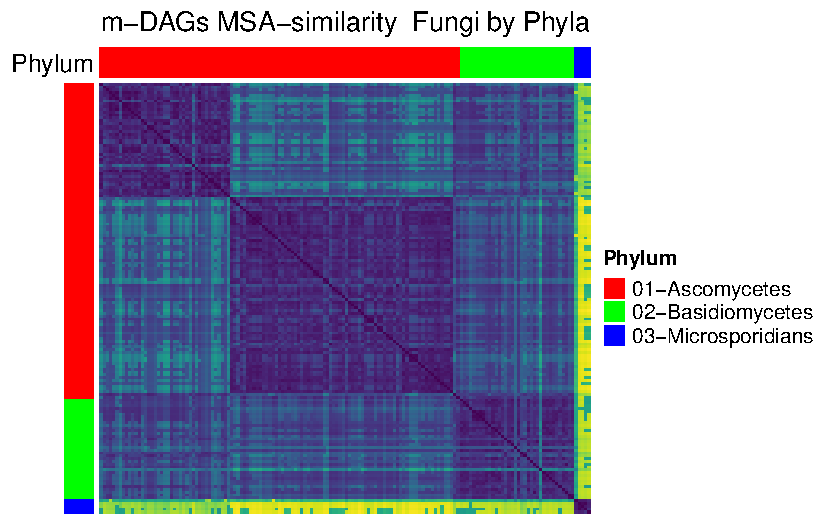
\includegraphics[width=1\textwidth,height=\textheight]{appendix_files/figure-pdf/unnamed-chunk-13-1.pdf}

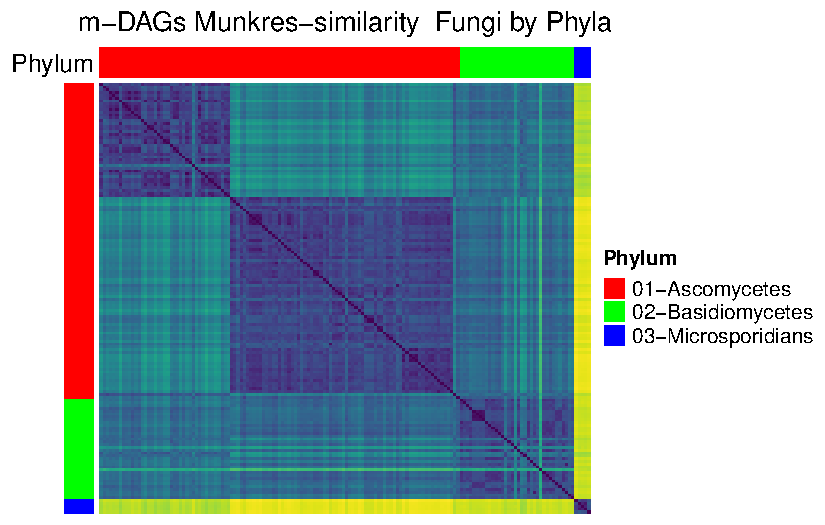
\includegraphics[width=1\textwidth,height=\textheight]{appendix_files/figure-pdf/unnamed-chunk-13-2.pdf}

\textbf{Protists}

\begin{Shaded}
\begin{Highlighting}[]
\NormalTok{meta\_protists}\OtherTok{=}\NormalTok{ meta\_taxo }\SpecialCharTok{\%\textgreater{}\%} \FunctionTok{filter}\NormalTok{(Kingdom}\SpecialCharTok{==}\StringTok{"Protists"}\NormalTok{)}

\NormalTok{namesP}\OtherTok{=}\FunctionTok{names}\NormalTok{(}\FunctionTok{rev}\NormalTok{(}\FunctionTok{sort}\NormalTok{(}\FunctionTok{table}\NormalTok{(meta\_protists}\SpecialCharTok{$}\NormalTok{Phylum))))}
\NormalTok{namesP}
\end{Highlighting}
\end{Shaded}

\begin{verbatim}
[1] "Alveolates"        "Euglenozoa"        "Stramenopiles"    
[4] "Amoebozoa"         "Metamonada"        "Choanoflagellates"
[7] "Heterolobosea"     "Haptophyta"        "Cryptomonads"     
\end{verbatim}

\begin{Shaded}
\begin{Highlighting}[]
\NormalTok{dff}\OtherTok{=}\FunctionTok{data.frame}\NormalTok{(}\AttributeTok{Phylum=}\NormalTok{meta\_protists}\SpecialCharTok{$}\NormalTok{Phylum)}
\NormalTok{Phylum}\OtherTok{=}\FunctionTok{ordered}\NormalTok{(meta\_protists}\SpecialCharTok{$}\NormalTok{Phylum,}\AttributeTok{levels=}\NormalTok{namesP)}
\NormalTok{n}\OtherTok{=}\FunctionTok{length}\NormalTok{(namesP)}
\NormalTok{numbersP}\OtherTok{=}\FunctionTok{paste}\NormalTok{(}\FunctionTok{c}\NormalTok{(}\FunctionTok{paste0}\NormalTok{(}\DecValTok{0}\NormalTok{,}\DecValTok{1}\SpecialCharTok{:}\NormalTok{n)),namesP,}\AttributeTok{sep=}\StringTok{"{-}"}\NormalTok{)}
\FunctionTok{levels}\NormalTok{(Phylum)}\OtherTok{=}\NormalTok{numbersP}
\NormalTok{dff}\SpecialCharTok{$}\NormalTok{Phylum}\OtherTok{=}\NormalTok{Phylum}
\NormalTok{col}\OtherTok{=}\FunctionTok{rainbow}\NormalTok{(}\FunctionTok{length}\NormalTok{(namesP))}

\NormalTok{colorsP}\OtherTok{=}\FunctionTok{list}\NormalTok{(}\AttributeTok{Phylum=}\NormalTok{col)}
\FunctionTok{names}\NormalTok{(colorsP}\SpecialCharTok{$}\NormalTok{Phylum)}\OtherTok{=}\NormalTok{numbersP}

\NormalTok{annot }\OtherTok{\textless{}{-}} \FunctionTok{HeatmapAnnotation}\NormalTok{(}\AttributeTok{df =}\NormalTok{ dff, }
                               \AttributeTok{col =}\NormalTok{ colorsP,}
                               \AttributeTok{annotation\_name\_side =} \StringTok{"left"}\NormalTok{,}
                               \AttributeTok{show\_annotation\_name=}\ConstantTok{TRUE}\NormalTok{ )}

\NormalTok{MSA\_heat\_2 }\OtherTok{\textless{}{-}}  \FunctionTok{Heatmap}\NormalTok{(}
  \AttributeTok{matrix =}\NormalTok{ Sim\_MSA\_mDAG[meta\_protists}\SpecialCharTok{$}\NormalTok{mDAG\_Id,}
\NormalTok{                        meta\_protists}\SpecialCharTok{$}\NormalTok{mDAG\_Id],}
  \AttributeTok{name =} \StringTok{"MSA similarity"}\NormalTok{,}
  \AttributeTok{column\_title =} \StringTok{"m{-}DAGs MSA{-}similarity  Protist by Phyla"}\NormalTok{,}
  \AttributeTok{col =} \FunctionTok{rev}\NormalTok{(}\FunctionTok{viridis}\NormalTok{(}\DecValTok{256}\NormalTok{)),}
  \AttributeTok{cluster\_rows =} \ConstantTok{FALSE}\NormalTok{,}
  \AttributeTok{show\_heatmap\_legend =} \ConstantTok{FALSE}\NormalTok{,}
  \AttributeTok{cluster\_columns =} \ConstantTok{FALSE}\NormalTok{,}
  \AttributeTok{top\_annotation =}\NormalTok{ annot,}
  \AttributeTok{show\_column\_names =} \ConstantTok{FALSE}\NormalTok{,}
  \AttributeTok{show\_row\_names =} \ConstantTok{FALSE}\NormalTok{,}
  \AttributeTok{left\_annotation =}
    \FunctionTok{rowAnnotation}\NormalTok{(}
      \AttributeTok{df =}\NormalTok{ dff,}
      \AttributeTok{col =}\NormalTok{ colorsP,}
      \AttributeTok{show\_annotation\_name =} \ConstantTok{FALSE}
\NormalTok{    )}
\NormalTok{)}

\NormalTok{Mun\_heat\_2 }\OtherTok{\textless{}{-}} \FunctionTok{Heatmap}\NormalTok{(}
  \AttributeTok{matrix =}\NormalTok{ Sim\_Mun\_mDAG[meta\_protists}\SpecialCharTok{$}\NormalTok{mDAG\_Id,}
\NormalTok{                        meta\_protists}\SpecialCharTok{$}\NormalTok{mDAG\_Id],}
    \AttributeTok{name =} \StringTok{"Mun similarity"}\NormalTok{,}
  \AttributeTok{column\_title =} \StringTok{"m{-}DAGs Munkres{-}similarity  Protist by Phyla"}\NormalTok{,}
\AttributeTok{col =} \FunctionTok{rev}\NormalTok{(}\FunctionTok{viridis}\NormalTok{(}\DecValTok{256}\NormalTok{)),}
  \AttributeTok{cluster\_rows =} \ConstantTok{FALSE}\NormalTok{,}
  \AttributeTok{show\_heatmap\_legend =} \ConstantTok{FALSE}\NormalTok{,}
  \AttributeTok{cluster\_columns =} \ConstantTok{FALSE}\NormalTok{,}
  \AttributeTok{top\_annotation =}\NormalTok{ annot,}
  \AttributeTok{show\_column\_names =} \ConstantTok{FALSE}\NormalTok{,}
  \AttributeTok{show\_row\_names =} \ConstantTok{FALSE}\NormalTok{,}
  \AttributeTok{left\_annotation =}
    \FunctionTok{rowAnnotation}\NormalTok{(}
      \AttributeTok{df =}\NormalTok{ dff,}
      \AttributeTok{col =}\NormalTok{ colorsP,}
      \AttributeTok{show\_annotation\_name =} \ConstantTok{FALSE}
\NormalTok{    )}
\NormalTok{)}
\end{Highlighting}
\end{Shaded}

Save graphics

\begin{Shaded}
\begin{Highlighting}[]
\FunctionTok{draw}\NormalTok{(MSA\_heat\_2,}\AttributeTok{merge\_legend=}\ConstantTok{TRUE}\NormalTok{)}
\end{Highlighting}
\end{Shaded}

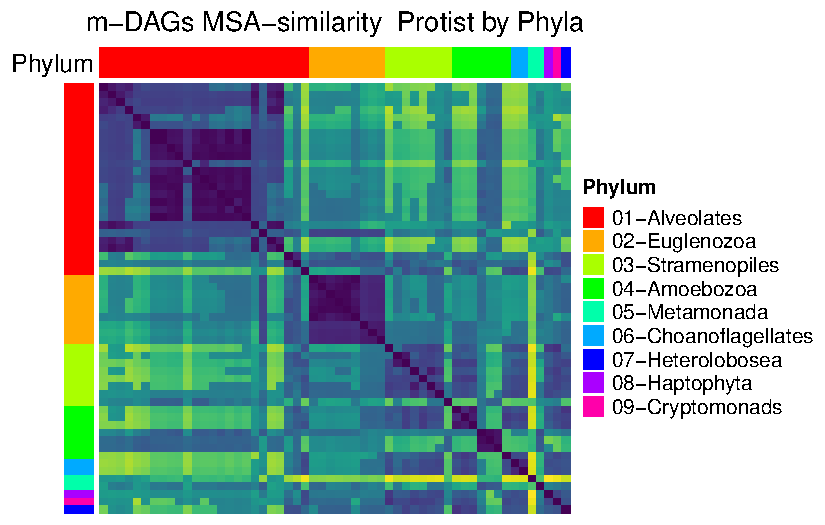
\includegraphics[width=1\textwidth,height=\textheight]{appendix_files/figure-pdf/unnamed-chunk-16-1.pdf}

\begin{Shaded}
\begin{Highlighting}[]
\FunctionTok{draw}\NormalTok{(Mun\_heat\_2,}\AttributeTok{merge\_legend=}\ConstantTok{TRUE}\NormalTok{)}
\end{Highlighting}
\end{Shaded}

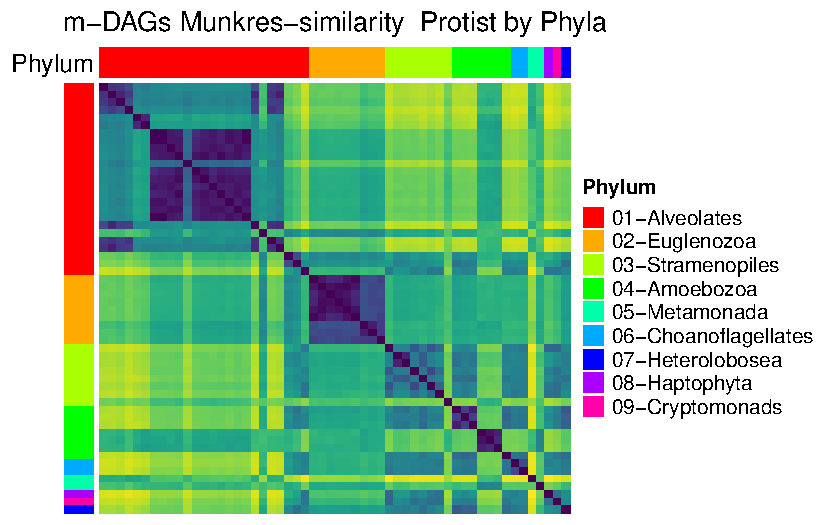
\includegraphics[width=1\textwidth,height=\textheight]{appendix_files/figure-pdf/unnamed-chunk-16-2.pdf}




\end{document}
